% !TEX root = ./thesis.tex

% DOC
\documentclass[openright,a4paper,12pt, twoside]{report}
\usepackage[
	includehead,
	hmargin={3.6cm, 2.6cm},
	vmargin={2.5cm,2.7cm},
	headsep=.8cm,
	footskip=1.2cm]{geometry}

% LINE SPACING
\usepackage{setspace}

% coloured frames
\usepackage{mdframed}
\mdfdefinestyle{todo}{
				leftmargin=5pt,
				linecolor=white,
				backgroundcolor=Red!10!White}
%
\newcommand{\todofr}[1]{
				\begin{mdframed}[style=todo]
					\vspace*{-.3cm}
					{\singlespacing\small#1}
					\vspace*{.1cm}
				\end{mdframed}}


% HEADERS
\usepackage{fancyhdr}
\setlength{\headheight}{15pt}
\fancyhf{} % clear the header and footers
\pagestyle{fancy}
\renewcommand{\chaptermark}[1]{\markboth{\thechapter. #1}{\thechapter. #1}}
\renewcommand{\sectionmark}[1]{\markright{\thesection. #1}}
\renewcommand{\headrulewidth}{0pt}
\fancyhead[LO]{\emph{\leftmark}}
\fancyhead[RE]{\emph{\rightmark}}
\fancyhead[RO,LE]{\emph{\thepage}}

% PART PAGE
\makeatletter
\renewcommand\part{%
  \if@openright
    \cleardoublepage
  \else
    \clearpage
  \fi
  \thispagestyle{empty}%   % Original »plain« replaced by »emptyx
  \null\vfil
  \secdef\@part\@spart}
\makeatother

% HYPERREF
\usepackage[colorlinks=true,
			linkcolor=TitleCol,
			citecolor=DarkGreen,
			urlcolor=TitleCol,
			linktocpage=true,
			pdfstartview=FitH]{hyperref}

% FONT
\usepackage[english]{babel}
\usepackage[utf8x]{inputenc}
\usepackage[T1]{fontenc}
\usepackage[default]{sourcesanspro}

%\usepackage[titles]{tocloft}
%\renewcommand{\cftchapfont}{\large\sc}

% COLORS
\usepackage[usenames,dvipsnames,svgnames]{xcolor}

\definecolor{TitleCol}{HTML}{28316C} % sections, ...
\definecolor{EnvCol}{HTML}  {28316C} % theorem, ...
\definecolor{CapCol}{HTML}  {28316C} % fig, ...

% CAPTIONS
\usepackage[width=.8\textwidth,					% caption width
			labelfont={bf,sf,color=CapCol},		% caption style
			font={footnotesize},
			format={hang},
			textfont={it}]{caption}

% CHAP STYLE
\usepackage{titlesec}
\makeatletter 			% section & subsection number in margin
	\def\@seccntformat#1{
		\protect\makebox[0pt][r]{
			\csname the#1\endcsname\quad
			}
		}
\makeatother

\titleformat*{\section}{
	\Large\bfseries\selectfont\color{TitleCol}}
\titleformat*{\subsection}{
    \large\bfseries\selectfont\color{TitleCol}}
\titleformat*{\subsubsection}{
    \small\bfseries\selectfont\color{TitleCol}}

% BIBLIOGRAPHY
\usepackage{natbib}

% TIKZ
\usepackage{tikz}
\usetikzlibrary{arrows,shapes}

% MATHS
\usepackage{amsmath}
\usepackage{amssymb}
\usepackage{amsthm}

\numberwithin{equation}{chapter}

% ALGORITHMS
\usepackage{algorithm}
\usepackage{algpseudocode}
\usepackage{algorithmicx}
% !TEX root = ./thesis.tex

%
% <D.1> Text
%
\newcommand{\begen} 		{\begin{enumerate}}
\newcommand{\stopen} 		{\end{enumerate}}
\newcommand{\noi}			{\noindent}
\newcommand{\fig}		[1] {\hyperref[#1]{figure \ref*{#1}}}
\newcommand{\nn}          	{\nonumber}
\renewcommand{\tt}		[1]	{\texttt{#1}}
\newcommand{\blue}		[1]	{\textcolor{blue}{#1}}
\newcommand{\dblue}		[1]	{\textcolor{Blue!70!NavyBlue}{#1}}
\newcommand{\blueit}	[1]	{\blue{\emph{#1}}}
\newcommand{\idblue}	[1]	{\dblue{\emph{#1}}}
\newcommand{\ddblue}	[1]	{\dblue{\textbf{#1}}}
\newcommand{\grayit}	[1]	{\gray{\emph{#1}}}
\newcommand{\dgray}		[1]	{\textcolor{Gray!80!Black}{#1}}
\newcommand{\idgray}	[1]	{\dgray{\emph{#1}}}
\newcommand{\dgreen}	[1]	{\textcolor{Black!40!OliveGreen}{#1}}
\newcommand{\dorange}	[1]	{\textcolor{Orange!40!Sienna}{#1}}
\newcommand{\red}		[1]	{\textcolor{red}{#1}}
\newcommand{\dred}		[1]	{\textcolor{BrickRed!60!Red}{#1}}
\newcommand{\idred} 	[1] {\dred{\emph{#1}}}
\newcommand{\clarify}	    {\dred{\textbf{\#\#\#\#}}\xspace}
\newcommand{\gray}		[1]	{\textcolor{Gray}{#1}}
\newcommand{\green}		[1]	{\textcolor{DarkGreen}{#1}}
\newcommand{\magenta}	[1]	{\textcolor{magenta}{#1}}
\newcommand{\orange}	[1]	{\textcolor{orange}{#1}}
\newcommand{\begar}			{\begin{itemize}[$\dblue{\rightarrow}$]\itsep{0}}
\newcommand{\stopar}		{\end{itemize}}
\newcommand{\itsep}		[1]	{\setlength{\itemsep}{#1pt}}
\newcommand{\hl}          	{\\\hline}


\newcommand{\ceil}         	[1] {\lceil#1\rceil}
\newcommand{\floor}        	[1] {\lfloor#1\rfloor}
\newcommand{\explainedrel} 	[2] {\stackrel{\dblue{\text{#1}}}{#2}}
\newcommand{\bstack} 		[2] {\stackrel{\dblue{\text{#1}}}{#2}}
\newcommand{\fracd} 		[2] {\frac{\partial #1}{\partial #2}}
\newcommand{\KL}			[1] {\mathrm{KL}\!\left(#1\right)}
\newcommand{\R}			    	{\mathbb R}
\newcommand{\st}		    	{\,|\,}
\newcommand{\sign}		  		{\mathrm{sign}\,}
\newcommand{\supp}				{\mathrm{supp}}

% Distributions
\newcommand{\Be}	 {\mathrm{Be}}
\newcommand{\Beta}	 {\mathrm{Beta}}
\newcommand{\Bi}	 {\mathrm{Bi}}
\newcommand{\Dir}	 {\mathrm{Dirichlet}}
\newcommand{\Expo}	 {\mathrm{Expo}}
\newcommand{\Gam}	 {\mathrm{Gamma}}
\newcommand{\iid}	 {\text{iid.}\xspace}
\newcommand{\Poi}	 {\mathrm{Poi}}
\newcommand{\simiid} {\sim_{\mathrm{iid.}}}

% Probability stuff
\newcommand{\E} {\mathbb E}
\newcommand{\V}	{\mathbb V}

% spacing
\newcommand{\esp}		{\quad\!\!}
\newcommand{\spe}		{\quad\!\!=\quad\!\!}
% norms
\newcommand{\norm}		[2]	{\left\|#1\right\|_{#2}}
	\newcommand{\anorm}	[1]	{\norm{#1}{1}}
	\newcommand{\bnorm}	[1]	{\norm{#1}{2}}
	\newcommand{\inorm}	[1]	{\norm{#1}{\infty}}
	\newcommand{\xnorm}	[1]	{\norm{#1}{}}

% formatting in equations
\newcommand{\abs}	[1]	{\left|#1\right|}
\newcommand{\eq}	[1]	{\begin{equation}#1\end{equation}}
\newcommand{\eqa}	[1]	{\begin{eqnarray}#1\end{eqnarray}}
\newcommand{\aleq}	[1]	{\begin{align}#1\end{align}}
\newcommand{\inv}		{^{-1}}
\newcommand{\transp}	{^\mathrm{t}}
\newcommand{\itransp}	{^{-\mathrm{t}}}
\newcommand{\pab}	[1]	{\left\{#1\right\}} % {	}
\newcommand{\pac}	[1]	{\left[#1\right]}	% [	]
\newcommand{\pat}	[1]	{\left(#1\right)}	% (	)
\newcommand{\syst}	[1]	{\left\{\begin{array}{r c l}#1\end{array}\right.}
\newcommand{\vb}	[1]	{\boldsymbol{#1}}
% vector operations
\newcommand{\grad}	[1]	{\pat{\begin{array}{c}#1\end{array}}}
\newcommand{\scal}	[1]	{\left\langle #1 \right\rangle}
% matrix operations
\newcommand{\matd}	[1]	{\pat{\begin{array}{cc}#1\end{array}}}
\newcommand{\matt}	[1]	{\pat{\begin{array}{ccc}#1\end{array}}}
\newcommand{\tr}		{\mathrm{tr\,}}

% Integral Measures
%
\newcommand{\dd}	{\,\mathrm{d}}			% straight d

\newcommand{\ds}	{\dd s}
\newcommand{\dt}	{\dd t}
\newcommand{\du}	{\dd u}
\newcommand{\dv}	{\dd v}
\newcommand{\dw}	{\dd w}
\newcommand{\dx}	{\dd x}
\newcommand{\dy}	{\dd y}
\newcommand{\dz}	{\dd z}


\newif\iftoc
\newif\ifintro
\newif\ifbgs
\newif\iftfs
\newif\iflbps
\newif\ifbgm
\newif\ifpbp
\newif\ifsnep
\newif\ifccl

\def\compileall{1}
\toctrue    \tocfalse
\introtrue  \introfalse
\bgstrue  	\bgsfalse
\tfstrue    	\tfsfalse
\lbpstrue 	%\lbpsfalse
\bgmtrue  	\bgmfalse
\sneptrue 	\snepfalse
\pbptrue   	\pbpfalse
\ccltrue     \cclfalse

\if\compileall1
    \toctrue
    \introtrue
    \bgstrue
    \tfstrue
    \lbpstrue
    \bgmtrue
    \sneptrue
    \pbptrue
    \ccltrue
\fi

\newcommand{\itsepa}{\itsep0} % adjust all itseps in one shot

\reversemarginpar
\newcommand{\margnote}[1]{\marginpar{\hfill\fontsize{8}{0}{\idblue{(#1)}}}}

\usepackage{xspace}
\usepackage[backgroundcolor=Yellow!30,
			textsize=tiny]{todonotes}
			
\makeatletter
\renewcommand*{\cleardoublepage}{\clearpage\if@twoside \ifodd\c@page\else
\hbox{}%
\thispagestyle{empty}%
\newpage%
\if@twocolumn\hbox{}\newpage\fi\fi\fi}
\makeatother
    
\renewcommand\margnote[1]{\xspace}
\renewcommand{\P}{\mathbb P}

\newcommand\nudx{\nu(\!\dx)}
\renewcommand\transp{^t}

\usepackage{longtable}

\newcommand{\bif}{\text{BIF}}
\newcommand{\tbif}{\widetilde{\bif}}
\newcommand{\htbif}{\widehat\tbif}
\newcommand{\pd}{\text{PD}}
\newcommand{\hpd}{\widehat\pd}

%%%%%%%%%%%%%%%%%%%%%%%%%%
% COMMANDS FOR REVIEWING %
%%%%%%%%%%%%%%%%%%%%%%%%%%
\renewcommand{\check}[1]{}
%\renewcommand{\check}[1]{
%	\todo{\textbf{checked}: #1}\xspace
%	}
\newcommand{\add}[1]{}
%\newcommand{\add}[1]{
%	\todo[backgroundcolor=red!20,linecolor=red]{
%		\textbf{add}: #1
%		}
%	\xspace
%}
\newcommand{\addref}[1]{}
%\newcommand{\addref}{
%	\todo[backgroundcolor=green!20,linecolor=green]{
%		\textbf{add citation}
%		}
%	}


%%%%%%%%%%%%%%%%
\begin{document}

\thispagestyle{empty}
% !TEX root = ../thesis.tex

\begin{center}
{\Large\bfseries Inference on Markov Random Fields:\\[.2cm]
Methods and Applications}\\[1cm]
{\large Thibaut Lienart}\\[.3cm]
University College, University of Oxford\\[1cm]
\emph{A thesis submitted for the degree of Doctor of Philosophy}\\[.3cm]
Michaelmas 2017\\[1.5cm]

{\large\bfseries Abstract}
\begin{flushleft}
This thesis considers the problem of performing inference on undirected graphical models with continuous state spaces. 
These models represent conditional independence structures that can appear in the context of Bayesian Machine Learning. 
In the thesis, we focus on computational methods and applications. 
The aim of the thesis is to demonstrate that the factorisation structure corresponding to the conditional independence structure present in high-dimensional models can be exploited to decrease the computational complexity of inference algorithms.
First, we consider the smoothing problem on Hidden Markov Models (HMM) and discuss novel algorithms that have sub-quadratic computational complexity in the number of particles used. 
We show they perform on par with existing state-of-the-art algorithms with a quadratic complexity. 
Further, a novel class of rejection free samplers for graphical models known as the Local Bouncy Particle Sampler (LBPS) is explored and applied on a very large instance of the Probabilistic Matrix Factorisation (PMF) problem. 
We show the method performs slightly better than Hamiltonian Monte Carlo methods (HMC). 
It is also the first such practical application of the method to a statistical model with hundreds of thousands of dimensions. 
In a second part of the thesis, we consider approximate Bayesian inference methods and in particular the Expectation Propagation (EP) algorithm. 
We show it can be applied as the backbone of a novel distributed Bayesian inference mechanism. 
Further, we discuss novel variants of the EP algorithms and show that a specific type of update mechanism, analogous to the mirror descent algorithm outperforms all existing variants and is robust to Monte Carlo noise. 
Lastly, we show that EP can be used to help the Particle Belief Propagation (PBP) algorithm in order to form cheap and adaptive proposals and significantly outperform classical PBP. 
\end{flushleft}
\end{center}

\cleardoublepage



% !TEX root = ../thesis.tex
\begin{titlepage}
\begin{center}

\vspace*{1.2cm}

{\Huge{\bfseries Inference on Markov Random Fields:\\[.1cm] Methods and Applications}\\}
\vfill 
\vspace*{-.3cm}
\includegraphics[scale=.8]{figures/oxlogo}
\vspace*{-.7cm}
\vfill

{\Large Thibaut Lienart}\\[.5cm]

{\large 
   	{Department of Statistics}}\\[0.3cm]
{\large 
   	{University College}}\\[0.5cm]
{\Large
	{\textsc{University of Oxford}}}
	
\vspace*{-.4cm}
\vfill

{\large A thesis submitted for the degree of}\\[.3cm]

{\large \emph{Doctor of Philosophy}}\\[.3cm]

{\large \dred{XXXXXXX} 2017}
%\vspace*{-.4cm}
\vfill
\end{center}
\end{titlepage}
\clearpage
\thispagestyle{empty}

\titleformat{\chapter}[hang]{\Huge\bfseries\sc\color{TitleCol}\raggedleft}{\thechapter\hspace{20pt}\textcolor{Gray}{$\mid$}\hspace{20pt}}{0pt}{\Huge\bfseries\color{TitleCol}\sc}


%%%% TABLE OF CONTENTS

\singlespacing
\setcounter{tocdepth}{2}
\setcounter{secnumdepth}{2}
\iftoc\tableofcontents\fi

\cleardoublepage
%%%% ACKNOWLEDGEMENTS
% !TEX root = ../thesis.tex

%\topskip0pt
%\vspace*{\fill}
{\large \bfseries \dred{Acknowledgments}}\\

\dred{Here acks}
%\vspace*{\fill}

\thispagestyle{empty}
%\clearpage

%%%% NOTATIONS / ABBREVIATIONS

\raggedbottom
% !TEX root = ../thesis.tex

\chapter*{Notations}

We list here notations used throughout the document that are considered to be commonly used in computational statistics. Non-standard notations will be introduced in the document explicitly.

\subsection*{Vectors, matrices and functions} 
For a vector $x\in\R^{d}$ we write $\norm{x}{p}$ the $p$-norm of $x$ with $\norm{x}{p}^{p}=\sum_{i=1:d}\abs{x_{i}}^{p}$ for $p\in[1,\infty)$. 
For $x,y\in\R^{d}$, we write $\scal{x,y}=\sum_{i=1:n}x_{i}y_{i}$ the inner product of $x$ and $y$. 
We denote the transpose of a matrix $A\in\R^{d\times d}$ by $A\transp$. $A$ is said to be semi positive definite if $\scal{x,Ax}\ge 0$ for all $x\in\R^{d}$ and positive definite if the inequality holds strictly for all $x\neq 0$. We denote by $\mathbb S_+^{d}\subset \mathbb R^{d\times d}$ the set of symmetric positive definite matrices and by $\mathbb S_-^{d}$ the set of matrices $B$ such that $-B\in\mathbb S_+^{d}$.
For a real-valued measurable function $f$ on a set $\mathcal X$, we write $\|f\|_{p}^{p}=\int_{\mathcal X} |f(x)|^{p}\dx$ the $p$-norm of $f$ for $p\in[1,\infty)$. 
We write $L^{1}(\mathcal X)$ the set of functions such that $\|f\|_{1}<\infty$ and $\mathcal P(\mathcal X) \subset L^{1}(\mathcal X)$ denotes the restriction to nonnegative functions integrating to one (probability density functions). 
For a real-valued, differentiable function $f$, we write $\nabla f$ its gradient and $\nabla^{2} f$ its Hessian provided $f$ is twice differentiable.\check{jun21,may10}
%
\subsection*{Probabilities and expected values}
We consider continuous sample spaces $\mathcal X\subseteq \R^{n}$ and, by default, we consider the associated Borel $\sigma$-algebra. 
Correspondingly, we use the shorthand $(\mathcal X,\P)$ to denote a probability space with $\P$ the probability measure. 
We consider probability measures that admit a probability density function $p$ with respect to a base measure $\nu$ with therefore $\P(x\in A)=\int_{A}p(x)\nudx$ for any open subset $A\subset \mathcal X$. 
In particular, $\mathcal N(\cdot; \mu,\Sigma)$ denotes the multivariate normal distribution function with mean $\mu\in \R^{d}$ and covariance matrix $\Sigma\in\mathbb S^{d}_+$. 
For such a probability space and a vector-valued mapping $\varphi:\mathcal X\to\R^{d}$, we write the expectation and the covariance matrix of $\varphi$ with respect to $p$ as $(\E_{p}[\varphi(X)])_{i}=\int_{\mathcal X}\varphi_{i}(x)p(x)\nudx$ and $\V_{p}[\varphi(X)]=\E_{p}[\varphi(X)\varphi(X)^{t}]-\E_{p}[\varphi(X)]\E_{p}[\varphi(X)]^{t}$ respectively. 
We write $\KL{p,q}=\E_{p}[\log p(X)]-\E_{p}[\log q(X))]$ the Kullback-Leibler divergence between two probability distribution functions $p$ and $q$ on $\mathcal X$. We write $X\sim p$ to denote a random variable associated to $p$ and $\{X^{(i)}\}_{i=1}^{N}\simiid p$ for a set of independent such random variables.\check{jun21,june15,june8,april27}
%

\subsection*{Convex analysis}
Let $B\subset\R^{n}$ denote the Euclidean unit ball with $B=\{x\in\R^{n}\mid \|x\|_{2}\le 1\}$. For any subset $C\subseteq\R^{n}$, we write $\mathrm{int}\,(C)$ the interior of $C$ with $\mathrm{int}\,(C)=\{x\in C \mid \exists \epsilon>0, x+\epsilon B \subset C\}$. Correspondingly we write $\mathrm{cl}(C)$ the closure of $C$ with $\mathrm{cl}(C) = \cap\{C+\epsilon B\st \epsilon>0\}$. A set $C$ is convex if for any $x,y\in C$, $(1-\lambda)x+\lambda y\in C$ for all $\lambda\in(0,1)$. Let $\Omega$ be an arbitrary connected and nonempty subset of $\R^{n}$; a function $f:\Omega\to\R$ is said to be convex if $f((1-\lambda)x+\lambda y)\le (1-\lambda)f(x)+\lambda f(y)$. For an arbitrary function $f:\Omega\to\R$, we denote by $f^{\star}:\R\to \R\cup\{+\infty\}$ the convex-conjugate of $f$ with $f^{\star}(y)=\sup_{y\in \Omega}[\scal{x,y}-f(x)]$. The set of minimisers of a function $f$ on a open, nonempty set $C$ is denoted by $\arg\min_{x\in C}\,f(x)$ i.e. the set $\pab{x\in C\mid f(y)\ge f(x), \,\forall y\in C}$. For a differentiable, strictly convex function $\varphi:C\to\R$, we denote by $B_\varphi(x,y)$ the Bregman divergence associated to $\varphi$ between $x$ and $y$ in $C$ with $B_\varphi(x,y)=\varphi(x)-\varphi(y)-\scal{x-y,\nabla \varphi(y)}$.  \check{jun21,may13}
%If the function $f$ is convex and differentiable on $C$ we call \emph{first-order condition} the fact that this set is equivalent to the set of points $x\in C$ such that $\nabla f(x)=0$.

%\dred{note} 
%\add{explain notations for message, explain add comma for t-1,t}
%
%\setlength{\tabcolsep}{12pt}
%\renewcommand{\arraystretch}{1.2}
%\begin{tabular}{ll}
%\textbf{symbol} 		& \textbf{meaning}\\[.3cm]
%$\mathcal X$ 			& sample space\\
%$x,y,z \in \mathcal X$	& sampling points\\
%$X,Y,Z$ 				& random variables\\
%$x_{1:T}$ 				& collection $\{x_{t}\}_{t=1}^{T}$\\
%$X \sim q(\cdot)$ 		& random variable drawn from a distribution $q$\\
%$\mathcal N(\,\cdot\,; \mu, \Sigma)$ 
%						& Normal distribution with mean $\mu$ and covariance matrix $\Sigma$\\
%%$p(x_{1:T})$ & joint distribution over the collection $\{x_{t}\}_{t=1}^{T}$\\
%$p(x\st y)$ 				& conditional distribution at $x$ given that $y$ was observed\\
%$\text{supp}(p)$ 		& set of $x$ such that $p(x)>0$ where $p$ is a distribution\\
%$\delta_{a}(x)$ 		& Dirac-delta distribution with point mass at $x=a$\\
%$\hat p(x)$ 				& \dred{particle estimator of the distribution $p$}\\
%%$\pd_t(x_t)$ & \dred{(in HMM) predictive density $p(x_t\st y_{1:t-1})$}\\
%%$\bif_t(x_t)$ & \dred{(in HMM) backward information filter $p(y_{t:T}\st x_t)$}\\
%%$\tbif_t (x_t)$ & \dred{(in HMM) normalised backward information filter $\gamma_t(x_t)p(y_{t:T}\st x_t)$}\\
%$\psi_{u}$ 				& singleton potential on a node $u$\\
%$\psi_{uv}$ 				& pairwise potential on an edge between a node $u$ and a node $v$\\
%$\partial i$ 			& neighbourhood of node $i$ in a graph\\
%$m_{st}$ 				& message from node $s$ to node $t$\\
%$M_{st}$ 				& \dred{pre-message at $s$ going to $t$ in Belief Propagation}\\
%$\KL{p,q}$ 				& Kullback-Leibler divergence between two distributions $p$ and $q$\\
%$\mathcal F_\phi$ 		& exponential family with sufficient statistic $\phi$\\
%$q_\theta$ 				& distribution parametrised by $\theta$\\
%$A(\nu)$ 				& log-partition function of an $\mathcal F_{\phi}$ distribution parametrised by $\theta$\\
%$A^{\star}(\nu)$		& \dred{convex-conjugate of $A$}\\
%%$\theta[q]$ & natural parameter of distribution $q\in \mathcal F_{\phi}$\\
%%$\mu[q]$ & mean parameter of distribution $q\in \mathcal F_{\phi}$\\
%\dred{$\mathcal P_\phi[p]$} 	& Kullback-Leibler projection of a distribution $p$ on $\mathcal F_\phi$\\
%$\E_p[\phi]$ 			& expected value of $\phi(X)$ if $X\sim p(\cdot)$\\
%$\V_{p}[\phi]$ 			& \dred{variance of $\phi(X)$} if $X\sim p(\cdot)$  
%
%\end{tabular}

\setlength{\tabcolsep}{6pt} % default
\subsection*{Abbreviations}
We list below abbreviations that are used in this document by alphabetical order. 
\add{add link to primary definition, check all are used}
\setlength{\tabcolsep}{12pt}
\renewcommand{\arraystretch}{1.2}
\begin{longtable}{ll}
BIF 		& Backward Information Filter\\
BB$\alpha$	& BlackBox $\alpha$-divergence minimisation algorithm\\
BP/LBP 		& (Loopy) Belief Propagation\\
EP	 		& Expectation Propagation\\
EPBP 		& Expectation Particle Belief Propagation\\
ESS 		& Effective Sample Size\\
FFBS 		& Forward Filtering Backward Smoothing \\
IPP 		& Inhomogeneous Poisson Process\\
HMM 		& Hidden Markov Model\\
MCMC 		& Markov Chain Monte Carlo\\
(L/G)MMC	& Local/Global Moment Matching Conditions (equations \ref{eq:LMMC},~\ref{eq:GMMC})\\
MRF 		& Markov Random Field (point \ref{subsection: mrf})\\
NBP 		& Nonparametric Belief Propagation\\
PBP	 		& Particle Belief Propagation\\
RMS(E) 		& Root Mean Squared (Error)\\
SMC 		& Sequential Monte Carlo\\
SMS 		& Sampling via Moment Sharing algorithm\\
SEP 		& Stochastic EP\\
SNEP		& Stochastic Natural gradient EP\\
TFS 		& Two Filter Smoothing\\ 
\end{longtable}
\setlength{\tabcolsep}{6pt} % default
\newpage


% --------------------------------------
% Now start the flushing + doublespacing

\doublespacing


%%%%%%%%%%%%%%%%%%%%%%
\chapter{Introduction}\setcounter{page}{1}\pagenumbering{arabic}

\ifintro% !TEX root = ../thesis.tex
%\section{Inference on Markov Random Fields}

In this thesis, we consider the framework of Bayesian inference in Machine Learning where one is interested in combining prior knowledge about the parameters of a given model with the likelihood of the observed data given the model. 
This combination of prior and likelihood leads to a posterior distribution on the parameters which is the key object of interest in Bayesian inference. This can be written
\eqa{
	p(\theta\st\mathcal D) &\propto& p(\mathcal D\st  \theta) p(\theta)
} 
where $p(\theta)$ is the prior distribution function over the parameter of interest $\theta$, $p(\mathcal D\st \theta)$ denotes the likelihood of the data $\mathcal D$ for a given model parameter and $p(\theta\st \mathcal D)$ is the posterior distribution over the parameters. 

We focus on the problem of estimating expected values with respect to such a posterior distribution and in particular with respect to its marginals. 
Further, we consider the case where the posterior factorises in a specific way and consider methods that attempt to leverage the factorisation structure to offer estimators at a reduced computational cost. 
The thesis concentrates on computational methods to tackle the problem in a number of important cases as well as applications and experiments. 

The thesis is divided in two parts. In the first part -- \emph{Sampling Methods} -- we consider ``exact'' methods that attempt to produce samples from the true marginals and lead to estimators of expectations of interest that are exact in the limit of infinite computational power and infinite precision in the representation of numbers. These methods can work well when the dimensionality of the state-space associated with the marginals of interest is not too high. 

In the second part -- \emph{Approximate Bayesian Inference} -- we consider approximate methods that attempt to find proxies for the marginals in restricted probability distribution spaces. These methods can offer a viable alternative to sampling methods when the latter become too expensive to consider. 

In this introductory chapter we introduce the concept of Markov Random Fields and present a few classical examples.

%%%%%%%%%%%
\section{\label{subsection: mrf}Markov Random Fields}
A \margnote{MRF}\emph{Markov random field} (MRF) is a graph structure that allows to represent joint distributions functions that factorise in a specific way or, in other words, to represent a set of conditional dependences between a set of random variables. In this document, we consider graphs determined by a finite index set $\mathcal V$, a set of edges $\mathcal E\subseteq \mathcal V\times \mathcal V$ connecting those nodes and \emph{potential functions} on its cliques (fully connected components of the graph). Each node $i\in\mathcal V$ corresponds to one random variable taking values in a sample space $\mathcal X_i \subseteq\mathbb R^{d_i}$ for some dimension $d_i\in\mathbb N$. 

We restrict ourselves to graphs with pairwise interactions i.e., uniquely determined by potential functions on their nodes and edges.\footnote{Considering only pairwise MRF is not too constraining since any MRF can be expressed as a pairwise MRF by the introduction of auxiliary variables although this may lead to a very complex graph \citet{wainwright08}.}
We write\check{sep14,jun22}
%
\eqa{	
	\psi_i : \mathcal X_i \to \mathbb R^{+}, \quad \text{and}\quad \psi_{ij}: \mathcal X_i\times \mathcal X_j \to \mathbb R^{+}, \nn	
}
% 
respectively a potential function on a node $i\in \mathcal V$ and on an edge $(i,j)\in \mathcal E$. 
%Note that, in principle, any MRF can be 
Such a graph represents the factorisation structure of a class of probability density functions on the product space $\mathcal X := \prod_{i\in \mathcal V}\mathcal X_{i}$ that can be written as
\eqa{		p(x) &\propto & \prod_{i\in\mathcal V}\psi_{i}(x_{i})\prod_{j\in\partial i}\psi_{ij}(x_{i},x_{j}),	}
where $x=(x_{i})_{i\in \mathcal V}$ and $\partial i:=\{j\st (i,j)\!\in\,\!\mathcal E\}$ denotes the \emph{neighbourhood} of the $i$th node. Note that any graphical model can be represented as a pairwise MRF \citep{yedidia00}. 
A simple pairwise MRF is illustrated in \fig{fig:simple-MRF}.\\

\begin{figure}[!h]
\center
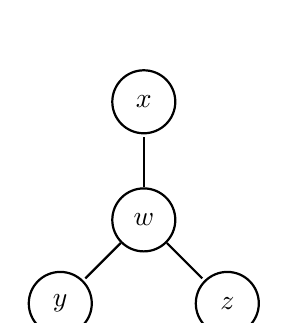
\begin{tikzpicture}[-,>=stealth',shorten >=1pt,minimum size=0.8cm,scale=.1,node distance=1.5cm, thick]
	\node[circle,draw] (A) 						{$w$};
	\node[circle,draw] (B) [above of=A] 		{$x$};
	\node[circle,draw] (C) [below right of=A] 	{$z$};
	\node[circle,draw] (D) [below left of=A] 	{$y$};
	
	\path 
	(A) edge	(B)
	(A) edge	(C)
	(A) edge	(D)
	;
\end{tikzpicture}
\caption{\label{fig:simple-MRF}Illustration of a simple MRF corresponding to distributions over 4 random variables admitting the following factorisation structure:\\ $p(w,x,y,z)\propto \psi_{w}(w)\psi_{x}(x)\psi_{y}(y)\psi_{z}(z)\psi_{wx}(w,x)\psi_{wz}(w,z)\psi_{wy}(w,y)$.}
\end{figure}
%The node potentials usually correspond to the likelihood of some observations $y_i$ (possibly a collection of observations) such that they can be written
%\eqa{ \psi_i(x_i) &=& p_i(y_i\st x_i),	\nn	}
%for some likelihood model $p_i$.
In this work, we are mainly concerned in determining or approximating  \emph{marginals}\margnote{marginals} on the MRF i.e. the distributions $p_{\mathcal I}(x_{\mathcal I})$ for $\mathcal I\subseteq\mathcal V$  with
\eqa{		p_{\mathcal I}(x_{\mathcal I}) &:=& \int p(x)\dx_{\mathcal V\backslash\mathcal I}	\label{eq:marginals}.}
A particular case of interest is\, $\mathcal I=\{r\}$ corresponding to the case of singleton marginals \citep[section 2.3]{wainwright08}. The integrals of the form \eqref{eq:marginals} are typically intractable but exploiting the underlying factorisation structure can lead to good approximation methods.\check{sep14, sep14, jun22}

We distinguish between two classes of undirected graph structures: the connected acyclic ones (\emph{trees}) and the rest (\emph{loopy graphs}). As we will show, computing marginals on a tree is relatively simple in comparison to doing so on loopy graphs. 
Among the trees, two graph structures are of particular interest in this document: the \emph{chain graph} and the \emph{star graph}. 
We also illustrate one specific type of loopy graph: the \emph{grid graph}.

%\dred{COULD ADD hierarchical model as tree graph}

%%%%%%%%%%%
\section{\label{intro:exMRF}Examples of MRF}
In this section, we present a brief overview of three examples of graph structures on which we will focus most of our effort throughout this document. 
We also present the type of applications they are connected with. 

%%%%%%%%%%%%%%
\subsection{Hidden Markov Models}
Chain graphs, where the random variables on every node take value in the same state-space $\mathcal X$, form the underlying structure of \emph{Hidden Markov Models} (HMM)\margnote{HMM} an important class of models. These can be illustrated as follows:
\begin{figure}[!h]
\center
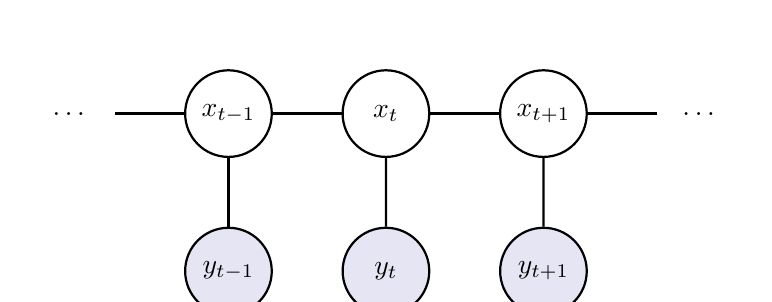
\begin{tikzpicture}[-,minimum size=1.1cm,scale=.1,node distance=2cm, thick]
	\node[circle,draw] (A) {$x_{t-1}$};
	\node[circle,draw] (B)[right of=A] {$x_{t}$};
	\node[circle,draw] (C) [right of=B] {$x_{t+1}$};
	\node[] (D) [right of=C] 	{$\dots$};
	\node[] (E) [left of=A]		{$\dots$};
	\node[circle,fill=DarkBlue!10,draw] (F) [below of=A] {$y_{t-1}$};
	\node[circle,fill=DarkBlue!10,draw] (G) [below of=B] {$y_{t}$};
	\node[circle,fill=DarkBlue!10,draw] (H) [below of=C] {$y_{t+1}$};
	
	\path 
	(A) edge	(B)
	(B) edge	(C)
	(C) edge	(D)
	(E) edge	(A)
	(A) edge (F)
	(B) edge (G)
	(C) edge (H)
	;
\end{tikzpicture}
\caption{\label{fig: hmm1} HMM with states $\{x_{t}\}_{t=1}^{T}$ and observations $\{y_{t}\}_{t=1}^{T}$.}
\end{figure}

HMMs are used in a broad range of applications from modelling time series data to speech processing (see for example \citet{ghahramani01, gales07, zucchini16}). In HMMs, the node potentials correspond to the likelihood of the corresponding observation and the edge potentials correspond to the \emph{transition density}:
\eqa{	\psi_t (x_t) &=& p(y_t\st x_t), \quad\text{and}\quad \psi_{t-1,t}(x_{t-1},x_t) \spe p(x_t\st x_{t-1}).	\nn}
A prior $\pi_{0}\in\mathcal P(\mathcal X)$ is assumed to be given for the first node so that we can write $p(x_1\st y_{1}) \propto \pi_{0}(x_1)p(y_1\st x_1)$. \check{sep14}

In the case of the HMM, obtaining or approximating the singleton marginals on the nodes from $1$ to $T$ given the observations $y_{1:T}$ is known as a \emph{smoothing problem}\margnote{smoothing}. The marginals or \emph{smoothing densities} can be written $p(x_t\st y_{1:T})$ to make explicit the dependence on all available observations.

A related problem is the \emph{filtering problem}\margnote{filtering} where one is only interested in building the last singleton marginal or, to put the problem in the same framework as before, to build marginals taking into account only the observations available until the point considered. This can be useful in an online setting where one is streaming data. 
The filtering densities are written $p(x_t\st y_{1:t})$. Correspondingly, we are often interested in representing the prediction density obtained by integrating the filtering densities with the transition density: 
%
\eqa{
	p(x_{t+1}\st y_{1:t}) &\propto& \int p(x_{t+1}\st x_{t}) p(x_{t}\st y_{1:t})\dx_{t}.
	}
%
%A related problem is to approximate the smoothing densities: $p(x_{t}\st y_{1:T}$). We will explore this in more details in chapter \ref{chap:BIS}. \check{jul24,june22}
%This is particularly relevant for applications such as time series analysis.\\

The \emph{linear-Gaussian} case is a particular instance of HMM, usually expressed as:
\eqa{	\syst{
			\pi_{0}(x_1) 				&=& \mathcal N(x_1; \mu_0, Q_0)	 	\\
			p(x_t\st x_{t-1}) 	&=& \mathcal N(x_t; A_t x_{t-1}+a_t, Q_t)		\\
			p(y_t\st x_t) 		&=& \mathcal N(y_t; B_t x_t+b_t, R_t)
		}
	\nn}
where $\mu_0$ as well as the $Q_t$, $R_t$, $A_t$, $a_t$, $B_t$ and the $b_t$ are fixed and deterministic. In such a case, an analytical expression for both the filtering and the smoothing densities can be obtained through the well-known \emph{Kalman filter} and \emph{Kalman smoother} \citep{anderson79}. \check{sep14}

However, in the general case where the transition is nonlinear and/or non-Gaussian, the marginals are typically intractable. Approximation algorithms such as \emph{Sequential Monte Carlo methods} (SMC) have been developed in order to generate approximate samples from these marginals and consequently be able to form Monte Carlo estimators. We introduce these methods in more detail in chapter \ref{chap:BGsampling}.
%We will show in this document a novel method to exploit a variational method known as \emph{expectation propagation} to help the performances of SMC smoothing algorithms. \dred{ADD SECTION NUMBER}

%%%%%%%%%%%%%%
\subsection{Star graphs}

In this document, we define \emph{star graphs}\margnote{star graph} as corresponding to a structure with a single random variable (possibly high-dimensional) with a node potential that factors into several likelihood terms. The structure is illustrated in figure \ref{fig:star1}. 

\begin{figure}[!h]
\center
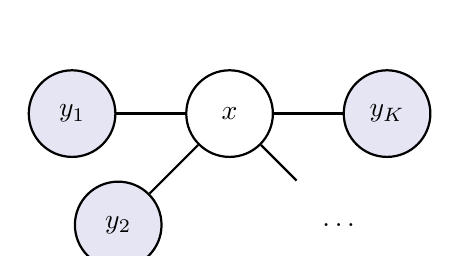
\begin{tikzpicture}[-,minimum size=1.1cm,scale=.1,node distance=2cm, thick]
	\node[circle,draw] (A) {$x$};
	\node[circle,fill=DarkBlue!10,draw] (B) [left of=A]		   {$y_{1}$};
	\node[circle,fill=DarkBlue!10,draw] (C) [below left of=A]  {$y_{2}$};
	\node[] (D) [below right of=A] {\dots};
	\node[circle,fill=DarkBlue!10,draw] (E) [right of=A]  {$y_{K}$};
	
	\path 
	(A) edge	(B)
	(A) edge	(C)
	(A) edge	(D)
	(A) edge (E)
	;
\end{tikzpicture}
\caption{\label{fig:star1} Star graph with hidden state $x$ and observations $\{y_k\}_{k=1}^{K}$. }
\end{figure} 

In this case, the singleton marginal can simply be written as:
\eqa{	p(x\st y) &\propto& \pi_0(x) \prod_{i=1}^{K} p(y_k\st x)	\nn}
where the $y_k$ are subsets of the entire observed data and $\pi_0$ is a prior on the hidden state. This can be a useful representation for distributed inference where each of the observation node can correspond to a distinct physical machine with a portion of the relevant data. We exploit this structure to suggest a novel way to approach distributed Bayesian inference in chapter \ref{chap:EPforDBI}.\check{sep14, jul24, jun21}

\subsection{Grid and loopy graphs}
The examples listed above do not exhibit cycles. An example of a common MRF structure with cycles which is encountered, for instance, in image processing, is the \emph{grid graph}\margnote{grid graph} illustrated in \fig{fig:grid1}.

\begin{figure}[!h]
	\center
	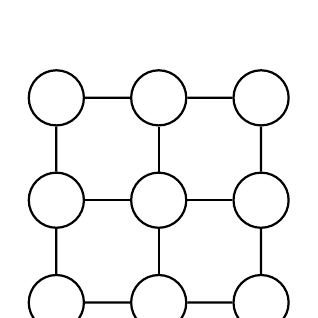
\begin{tikzpicture}[-,minimum size=.7cm,scale=.1,node distance=1.3cm, thick]
		\node[circle,draw] (A){};
		\node[circle,draw] (B) [left  of=A] {};
		\node[circle,draw] (C) [right of=A]{};
		\node[circle,draw] (D) [below of=A]{};
		\node[circle,draw] (E) [above of=A]{};
		\node[circle,draw] (F) [above of=B]{};
		\node[circle,draw] (G) [above of=C]{};
		\node[circle,draw] (H) [below of=B]{};
		\node[circle,draw] (I) [below of=C]{};
		\path
		(A) edge (B)
		(A) edge (C)
		(A) edge (D)
		(A) edge (E)
		(B) edge (F)
		(B) edge (H)
		(C) edge (I)
		(C) edge (G)
		(F) edge (E)
		(E) edge (G)
		(H) edge (D)
		(D) edge (I)
		;
	\end{tikzpicture}
\caption{\label{fig:grid1} Generic structure of a grid graph.}
\end{figure}

In image processing, grid graphs can be used to model interactions between the pixels of an image  \citep{blake11}. 
In the case of image denoising for example, for each pixel $k$ a noisy value $y_k$ is observed and we can have a model for the likelihood of $y_k$ given the true pixel value $x_k$ in the form $p(y_k\st x_k)$. These  form the node potentials. 
Additionally, we may have a similarity measure which can be used to penalise neighbouring pixels being very dissimilar. These form the edge potentials.\\
The problem of finding or approximating the singleton marginals then corresponds to finding the likelihood of a particular pixel taking a specific value given all the noisy observations available. We consider the problem of approximating marginals on such loopy graphs in chapter \ref{chap:EPBP}. \check{sep14, jul24,jun21}

\section{Exact vs Inexact Methods and Structure of the Thesis}

While the unifying theme of this thesis is the inference problem on Markov Random Fields, we consider two rather different approaches forming the two main parts of the thesis. In the first approach -- \emph{sampling methods} -- we consider methods to produce samples from the target densities (marginals of an MRF) from which Monte Carlo estimators can be computed. These methods take the form of stochastic processes which, asymptotically, are guaranteed to generate samples from the target distribution. These methods are considered ``exact'' because, asymptotically, they yield samples from the correct distribution. The difficulty of course is to assess whether the generating process has converged in the context of finite compute time and finite precision arithmetics. 

In the second approach -- \emph{approximated Bayesian inference} -- we consider methods to produce proxies to the target densities and compute expected values with respect to these proxies. These methods are considered ``inexact'' because even in the limit of infinite computational power or infinite precision arithmetic they do not lead to the correct expected values. 

Formally, let us denote $p$ a target distribution of interest and $\varphi$ a test function and put ourselves in the realistic context of finite computational power and precision. The aim is to compute the expected value of $\varphi$ with respect to $p$ or $\E_{p}[\varphi(X)]$. The first class of methods generates incorrect samples $\{\hat x_{1},\dots,\hat x_{n}\}$ which are hopefully statistically not too far from exact (but inaccessible) samples $\{x_{1},\dots,x_{n}\}$ drawn iid from $p$. 
As will be covered in section \ref{sec:MC+SMC}, the expected value of interest will be approximated as $\E_{p}[\varphi(X)]\approx n\inv \sum_{i=1:n}\varphi(\hat x_{i})$. The second class of methods attempts to find a simple distribution $q$ which is close in some sense to the target distribution $p$, the expected value of interest is consequently approximated as $\E_{p}[\varphi(X)]\approx \E_{q}[\varphi(X)]$. 

These two approaches rely on different set of tools. 
The first one relies primarily on particle methods while the second relies more heavily on optimisation tools. 
To simplify the presentation of the thesis, we therefore have two background chapters beginning each of the two parts. Each part is then formed of two chapters covering a specific method and discussing applications.


%The two approaches consider fairly different tools as 
%
%For both hard to assess qual... 



\fi

%%%%%%%%%%%%%%%%%%%%%%%%%%
\part{Sampling Methods} % part I

%%%%%%%%%%%%%%%%%%%%
\chapter{\label{chap:BGsampling}Background}

\ifbgs% !TEX root = ../thesis.tex

\section{Monte Carlo estimators}

\subsection{\dred{Review heavily}}

In the first case,\add{what first case} one is interested in computing the expected value of a test function $\varphi$ with respect to a distribution $\pi:\mathbb R^{d} \to \mathbb R_+$ i.e.: $I:=\E_\pi[\varphi(X)]$. Assuming it can't be computed analytically, a general approach is to consider a quadrature rule of the form:
%
\eqa{
	I\esp\approx\esp \widehat I_n &=& \sum_{i=1}^{n} w(X^{(i)}) \varphi(X^{(i)})
}
%
for some points $X^{(i)}\in\mathcal X$ and corresponding weights $w(X^{(i)})\in\mathbb R_+$. In low dimensions, we can consider deterministic quadrature rules such as the Gauss-Hermite quadrature. However, as the dimensionality increases, these deterministic rules tend to perform poorly even for a large number of integration points (``curse of dimensionality''). In that case, one can fall back to Monte Carlo integration with
%
\eqa{	
	X^{(i)}\esp \simiid\esp \pi(\cdot),\quad\text{and}\quad w(X^{(i)})\spe n^{-1}. 	
}
%
The strong law of large numbers then indicates that $\widehat I_n\to I$ almost surely with approximation error scaling like $\mathcal O(n^{-1/2})$ independently of the dimensionality of the problem. This is to be compared with deterministic rules which typically have approximation error scaling like $\mathcal O(n^{-\alpha/d})$ for a fixed $\alpha>0$ depending on the quadrature rule.

The problem then becomes one of drawing iid.\ samples from $\pi$. Often, this is also a hard problem and one can consider \emph{importance sampling} (IS)\margnote{IS} whereby samples are drawn from a \emph{proposal distribution}\margnote{proposal} $q\approx \pi$ and the quadrature weights are adjusted to reflect that:
%
\eqa{
	X^{(i)}\esp \simiid\esp q(\cdot), \quad\text{and}\quad w(X^{(i)})\spe {\pi(X^{(i)})\over n q(X^{(i)})}.
} 
%
Provided the support of $q$ englobes that of $\pi$ i.e., $\pi(x)>0\Rightarrow q(x)>0$ and provided that $\E_q[\abs{\varphi(X)}w(X)]$ is bounded, the importance sampling estimator is unbiased and consistent.\check{apr1}


\fi

%%%%%%%%%%%%%%%%%%%%%%%%%%%%%%
\chapter{\label{chap:BIS}Backward Information Smoothing}

\iftfs% !TEX root = ../thesis.tex

%%%%%%%%%%%%%%%%%%%%%%%%%%%%
\section{Two Filter Smoothing}
\add{Clarify where this comes from (marginal on HMM)}In this chapter, we focus on the problem of approximating the smoothing distributions for a Hidden Markov Model (HMM).\add{specify HMM more specifically, in particular state space} 
We assume that a sequence of empirical densities approximating the filtering distributions has already been obtained through a particle filtering step.
We had seen at point \ref{bg:particle-smoothing} that the \emph{forward filtering backward smoothing} algorithm (FFBS) recycles a particle filter and simply updates its weights. 
The issue with this approach is that no particles are resampled in the backward step. As we mentioned\add{link} this can impact the performances of the estimators if the support of the filtering distributions and that of the smoothing distributions don't overlap well.\add{maybe show this in FFBS case}

\subsection{Two filter formula}
An alternative to the FFBS approach is to exploit the \emph{two filter formula}. 
To derive it, note that the smoothing distribution can be written in the following way using Bayes' formula:
%
\eqa{
	p(x_t\st y_{1:T})&=& {p(x_t,y_{1:t-1},y_{t:T})\over p(y_{1:T})}.\nn
	}
% 
Then, exploiting the conditional dependences of the HMM, we get
%
\eqa{
	p(x_t\st y_{1:T}) 	
		&\propto& p(y_{t+1:T}\st x_t,x_{t+1},y_t)p(y_t\st x_t,x_{t+1})
\nn\\
		&\propto& p(x_t\st y_{1:t-1})p(y_{t:T}\st x_t).	\label{eq:TFS}
}
%
This last factorised form is the two filter formula which leads to the \emph{two filter smoothing} (TFS) algorithm \citep{bresler86, kitagawa96}. 
The first term in \eqref{eq:TFS} is the prediction density (PD), 
the second term $p(y_{t:T}\st x_{t})$ is called the \emph{backward information filter} (BIF). To simplify developments we introduce the following non-standard notations for the predictive density and the backward information filter:
%
\eqa{
	\pd_{t}(x_{t}) \esp:=\esp p(x_{t}\st y_{1:t-1}), \quad\text{and}  \quad \bif_{t}(x_{t}) \esp:=\esp p(y_{t:T}\st x_{t}).
}
%
The prediction density is obtained by integrating the filtering density multiplied by the transition density:\add{add reference to MRF part where introduced}
%
\eqa{
	\pd_{t}(x_{t}) &=& \int p(x_{t}\st x_{t-1})p(x_{t-1}\st y_{1:t-1})\dx_{t-1}.\label{eq:pred-dens}
}
%
an approximation to the prediction density can therefore easily be obtained by plugging a particle representation of the filtering density in \eqref{eq:pred-dens}. \check{july5}
%%%%%%%%%%%%%%%%%%%%%%%%%%
\subsection{Targeting the backward information filter}
The backward information filter cannot be directly targeted in a SMC framework in general as it may not be proportional to a distribution in $x_{t}$. 
In \citet{briers10}, the authors therefore suggest to introduce a sequence of artificial \emph{normalisation densities} $\{\gamma_{t}\}_{t=1}^{T}\in\mathcal P(\mathcal X)$ such that, for each step $t$, the product of $\gamma_{t}$ and $\bif_{t}$ is normalisable. 
In other words, the normalising distribution $\gamma_{t}$ allows to define a \emph{normalised backward information filter} in $\mathcal P(\mathcal X)$ with
%
\eqa{
	\tbif_{t}(x_{t}) &:=& Z\inv_{t}\gamma_{t}(x_{t})\bif_{t}(x_{t})
}
%
for some normalising constant $Z\inv_{t}$.\check{july5}
Any $\gamma_{t}\in\mathcal P(\mathcal X)$\add{make sure it's clear that every node is on same space $\mathcal X$} can be chosen as long as it verifies the \emph{support condition} i.e.: as long as its support covers that of the backward information filter:
%
\eqa{	
	\bif_t(x_t) &>&0 \quad\Longrightarrow\quad \gamma_{t}(x_{t})\esp>\esp 0. \label{eq: tech condition normalisation density}	
}
%
In order to target the sequence of normalised BIF in a SMC framework, it is useful to show that it verifies a factorisation structure similar to that of the filtering distribution. For this, we start by noting that
%
\eqa{		
	p(y_{t:T}\st x_{t},x_{t+1}) 
		&=& p(y_{t+1:T}\st x_{t},x_{t+1},y_{t})p(y_{t}\st x_{t},x_{t+1})\nn\\
		&=& p(y_{t}\st x_{t}) \bif_{t+1}(x_{t+1}). \label{back rec 1}	
}
%
On the other hand, we also have that
%
\eqa{		
	p(y_{t:T}\st x_{t},x_{t+1}) 	
		&=& {p(y_{t:T},x_{t},x_{t+1})\over p(x_{t+1}\st x_{t})p(x_{t})}\nn\\
		&=&{p(x_{t+1}\st x_{t},y_{t+1:T})\text{BIF}_{t}(x_{t})\over p(x_{t+1}\st x_{t})},	\label{back rec 2}
}
%
where we have used the conditional independence structure of the HMM. 
Combining \eqref{back rec 1} and \eqref{back rec 2} then leads to\check{july5}
%
\eqa{	
	\bif_{t}(x_{t}) p(x_{t+1}\st x_{t},y_{t+1:T}) &=& p(y_{t}\st x_{t})p(x_{t+1}\st x_{t})\bif_{t+1}(x_{t+1}). 	\label{eq:tfs-bif2}
}
%
If we now introduce the normalisation densities $\gamma_{t}$ and $\gamma_{t+1}$ and the corresponding normalisation constants $Z_{t}$ and $Z_{t+1}$ in \eqref{eq:tfs-bif2} we get\check{july5}
%
\eqa{	 
	\tbif_{t}(x_{t})p(x_{t+1}\st x_{t},y_{t+1:T}) &=& 
		{Z_{t+1}\gamma_{t}(x_{t})\over Z_{t}\gamma_{t+1}(x_{t+1})}p(y_{t}\st x_{t})p(x_{t+1}\st x_{t})\tbif_{t+1}(x_{t+1}).		\nn
}
%
By construction of the normalisation densities, we can integrate the previous expression over $x_{t+1}$ to obtain
%
\eqa{		
	\tbif_{t}(x_{t}) &\propto& {\gamma_{t}(x_{t})}p(y_{t}\st x_{t})\int p(x_{t+1}\st x_{t}){\tbif_{t+1}(x_{t+1})\over \gamma_{t+1}(x_{t+1})}\dx_{t+1}.	\nn
}
%
Noting that $\bif_{T}(x_{T})=p(y_{T}\st x_{T})$ and iterating brings
%
\eqa{		
	\tbif_{t}(x_{t}) &=& \int {\gamma_{t}(x_{t})}\prod_{\ell=t}^{T-1}p(x_{\ell+1}\st x_{\ell})\prod_{k=t}^{T}p(y_{k}\st x_{k})\dx_{t+1:T}.	\nn
}
%
We can thus define a joint distribution $\tbif_{t}(x_{t:T})$ as the integrand of the above expression with the following sequential structure:
\eqa{		\tbif_{t}(x_{t:T}) &\propto& {\gamma_{t}(x_{t})p(x_{t+1}\st x_{t})p(y_{t}\st x_{t})\over \gamma_{t+1}(x_{t+1})}\tbif_{t+1}(x_{t+1:T}),	\label{recursion joint BIF}}
which lends itself well to the SMC framework with the optimal proposal:
%
\eqa{
	q^{\text{opt}}_{t}(x_{t}\st x_{t+1}) &\propto& {\gamma_{t}(x_{t})p(x_{t+1}\st x_{t})p(y_{t}\st x_{t})\over \gamma_{t+1}(x_{t+1})}.
}
%
\check{july5}
%%%%%%%%%%%%%%%%%%%%%%%%%%%%%
\subsection{\label{introTFS}Two filter smoothing algorithm}
Plugging a particle representation of the filtering distribution in \eqref{eq:pred-dens}, the prediction density can be approximated by
%
\eqa{
	\widehat\pd_t(x_t)  &=& \sum_{i=1}^{N} w^{(i)}_{t-1}p(x_{t}\st X^{(i)}_{t-1}).	
\label{eq PDhat}	
}
%
Correspondingly, we can consider a particle representation of the normalised BIF obtained by following a backward particle filter with $M$ particles on \eqref{recursion joint BIF}. 
%The non-standard notation $\pd_{t}$ as well as the notations introduced below for the backward information filter will make the discussion of the TFS algorithm simpler and less cluttered. The backward information filter $\bif_t(x_t):=p(y_{t:T}\st x_{t})$ is not necessarily proportional to a distribution in $x_{t}$ and can thus not be directly targeted in a SMC context. However, one can define an auxiliary quantity by pre-multiplying the backward information filter by an artificial \emph{normalisation density} $\gamma_{t}(x_{t})$ such that the product
%%
%\eqa{		
%	\tbif_t(x_t) &:=& Z_{t}\inv{\gamma_{t}(x_{t}) p(y_{t:T}\st x_t)},		\label{def normalised BIF}
%}
%%
%is a distribution in $x_{t}$ (with $Z_{t}$ a normalisation constant) and can thus be targeted in the SMC framework \citep{briers10}.\check{jun24} 
%We will refer to these densities as \emph{normalisation densities}. The $\tbif_{t}$ are distributions and can be targeted in a SMC framework. 
Let us denote these by $\widehat\tbif_{t}$ with weights $\tilde w_{t+1}^{(j)}$ and particles $\tilde X^{(j)}_{t+1}$, i.e.:
%
\eqa{		
	\widehat\tbif_t(x_t) &=& \sum_{j=1}^{M} \tilde w^{(j)}_{t+1} \delta_{\tilde X^{(j)}_{t+1}}(x_{t}).
	} 
%
By dividing these by the corresponding normalisation density $\gamma_{t}$, we can obtain approximations to the original BIF:
%
\eqa{		
	\widehat\bif_t(x_t) &=& { \widehat\tbif_t(x_t)/  \gamma_{t}(x_{t})}.	\nn
}
%
Combining both the estimators of the prediction density and the backward information filter at step $t$, we can obtain a particle representation of the smoothing distribution with\check{jul5}
%
\eqa{		
	\hat{p}(x_{t}\st y_{1:T}) &=& \zeta_{t}\inv\widehat\pd_t(x_t)\widehat\bif_t(x_t)	, \label{first smoothing estimator}	
	}
%
where $\zeta_{t}$ is a normalisation constant.
That is a mixture of $NM$ terms and a further step may be desirable to reduce the number of components in the resulting representation of the smoothing distribution.
In particular, if we take $M=N$, at each step we have to consider a mixture with a quadratic number of terms in $N$ and this, independently of the choice of normalising densities meaning that the algorithm has inherently a quadratic complexity. We consider this choice in what follows and will come back to it in the discussion section.\add{come back to last sentence}\check{jul5}
%Note that since both the predictive density and the normalised BIF have been approximated using $N$ particles, the above estimator is a mixture of $N^{2}$ components and a further resampling step can be applied to reduce it to a mixture of only $N$ components. %\add{This is what Fearnhead does}

%Another comment that we can make at this point is that the form of the estimator in \eqref{first smoothing estimator} suggests taking as normalisation densities the estimator of the prediction densities. \\

%We will show explicitly how to implement the two filter smoothing algorithm with a near-ideal normalisation density in \hyperref[sec:TFS]{section \ref*{sec:TFS}}. 


%\todofr{
%\begin{itemize}
%	\item Add here the algorithm
%	\item add short discussion (complexity, choice of normalisation)
%\end{itemize}
%}


%%%%%%%%%%%%%%%%%%%%%
\section{Backward Information Smoothing}
In this section, we explore the choice of normalisation densities and suggest using an approximation to the predictive density. It came to our knowledge that this choice had in fact also been studied independently and earlier than this work by \citet{taghavi12}. 

%%%%%%%%%%%%%%%%%%%%%%%
\subsection{Choice of normalisation densities}
The choice of normalisation densities in the TFS algorithm is, in theory, only constrained by the support condition \eqref{eq: tech condition normalisation density}. However, the quality of the corresponding estimators for a finite sample size depends significantly on it. \add{explain Fearnhead / Briers choice and explain why it's not ideal}
Combining \eqref{eq:TFS} and \eqref{recursion joint BIF}, we get
%
\eqa{
	p(x_{t}\st y_{t:T}) &\propto& {\pd_{t}(x_{t})\over \gamma_{t}(x_{t})} \int \tbif_{t}(x_{t:T}) \dx_{t+1:T}\nn
}
%
so that we can write
%
\eqa{		
	p(x_{t:T}\st y_{1:T}) &\propto& {\pd_{t}(x_{t})\tbif_{t}(x_{t:T})\over \gamma_{t}(x_{t})}	\label{normalised BIF and partial joint}.
}
%
This expression suggests picking $\gamma_{1}$ to be the prior distribution on the first state $\pi_{0}(x_{1})$ since that leads directly to 
%
\eqa{		
	p(x_{1:T}\st y_{1:T}) &=& \tbif_{1}(x_{1:T}).	\label{full joint and first bif}
	}
%
The last two equations \eqref{normalised BIF and partial joint} and \eqref{full joint and first bif} are crucial for the rest of the analysis.\check{jul5} The first one suggests that if we pick $\gamma_{t}$ to be close to the predictive density then, then each term $\tbif_{t}(x_{t:T})$ forms an estimator for the partial joint smoothing densities $p(x_{t:T}\st y_{1:T})$; the second one indicates that upon selecting $\gamma_{1}$ to be the prior for the initial state, we end up targeting exactly the joint distribution of interest, no matter which admissible sequence $\{\gamma_{t}\}_{t=2}^{T}$ we picked earlier. 

This suggests to build a good estimator of the prediction density, based partly or entirely on a particle estimator of the filtering density; use it as normalisation density and target the corresponding normalised BIF recursively. 
We explored this idea and showed that it significantly outperforms the default choice used in \citep{briers10, fearnhead10}.\check{jul5}

Upon selecting $\gamma_{t}$ to be the approximation of the predictive density \eqref{eq PDhat} based entirely on a a particle estimator of the filtering density, we get what Taghavi calls the \emph{backward informations smoothing} (BIS) algorithm. \add{discuss with Arnaud: verifies support condition? -> yes if the support of $p(x_{t}\st x_{t-1})$ is the whole of $\mathcal X$}
The optimal importance function for targeting the corresponding normalised BIF is obtained by considering \eqref{recursion joint BIF} with this specific choice of normalising density:\check{jul2}\add{explain Xtilde}
\eqa{		\tilde q^{\text{opt}}_{t}(x_{t}\st \tilde X^{(j)}_{t+1}) &\propto & {\hpd_{t}(x_{t})\over \hpd_{t+1}(\tilde X^{(j)}_{t+1})} p(\tilde X^{(j)}_{t+1}\st x_{t})p(y_{t}\st x_{t}),\label{eq:opt-prop-bif}}
where the $\{\tilde X_{t+1}^{(j)}\}_{j=1}^{N}$ are the particles from the previous smoothing step. These steps are illustrated in algorithm \ref{alg:bisquad}.\check{jul5}

%
\begin{algorithm}[!h]\small
	\caption{\label{alg:bisquad}\dblue{\emph{\small Skeleton of a backward information smoother}}}
	\begin{algorithmic}[1]
		\State run a PF targeting $\{p(x_{t}\st y_{1:t})\}_{t=1}^{T}$ with $N$ particles $\{X^{(i)}_{t}, w^{(i)}_{t}\}_{t,i=1}^{T,N}$
		\For{$t=T-1:2$}
			\State sample $\tilde X^{(j)}_{t}\simiid \tilde q_{t}(\cdot\st \tilde X^{(j)}_{t+1})$ with $\tilde q_{t}\approx \tilde q_{t}^{\text{opt}}$ for $j=1,\dots,M$
			\State update and normalise the weights $\tilde w^{(j)}_{t}\propto \tilde\alpha^{(j)}_{t}\tilde w^{(j)}_{t+1}$
		\EndFor\\
		\Return weighted set of particles $\{\tilde X^{(j)}_{1:T}, \tilde w^{(j)}_{1:T}\}$
	\end{algorithmic}
\end{algorithm}
%

At each step $t$ and for each particle $j$, the algorithm \ref{alg:bisquad} ideally requires sampling a particle from $\hpd_{t}(x_{t})p(\tilde X^{(j)}_{t+1}\st x_{t})p(y_{t}\st x_{t})$ which is a mixture of $N$ terms. Additionally, computing the updating factors for the weights requires computing a sum of $N$ terms $\hpd_{t+1}(\tilde X_{t+1}^{(j)})$. Provided we use $N$ particles to target the BIF, the complexity of the BIS algorithm is therefore inherently quadratic in the number of particles as the FFBS algorithm.\check{jul5}

As it is not trivial in general to sample from $p(\tilde X^{(j)}_{t+1}\st x_{t})p(y_{t}\st x_{t})$, let alone when it is combined with $\hpd_{t}(x_{t})$, a possibility akin to the bootstrap proposal for the particle filter is to simply sample from $\hpd_{t}(x_{t})$. The disadvantage is that this choice doesn't take into account all the information available (contained in $\tilde X^{(j)}_{t}$ and $y_{t}$). Assuming we can sample easily from the transition distribution, sampling from $\hpd_{t}$ can be done easily in two steps: first sample an index $i^{\star}\sim \mathcal M(w^{(1)}_{t-1}, \dots, w^{(N)}_{t-1})$ where $\mathcal M$ denotes a multinomial distribution and then sample from the corresponding term $p(x_{t}\st X^{(i^{\star})}_{t-1})$. This procedure has linear complexity in the number of particles. The update factor is then given by
%
\eqa{
	\tilde\alpha^{(j)}_{t} &=& { p(\tilde X^{(j)}_{t+1} \st \tilde X^{(j)}_{t})p(y_{t}\st \tilde X^{(j)}_{t}) \over \hpd_{t+1}(\tilde X^{(j)}_{t+1})},
}
%
which also has linear complexity in the number of particles so that, as expected, the \emph{bootstrap backward information smoother} also has quadratic complexity.\check{jul5}

%%%%%%%%%%%%%%%%%%%%%%%%
\subsection{From quadratic to linear complexity}
%
We have shown that the BIF algorithm is inherently quadratic in the number of particles given the form of the optimal proposal \eqref{eq:opt-prop-bif}. A statistically equivalent way of writing the optimal sampling step is to suggest sampling $N$ particles from a mixture of $N^{2}$ terms: 
%
\eqa{
	\tilde X^{(j)}_{t} &\simiid & q^{\text{mix}}_{t} \esp\propto\esp \sum_{i,j=1}^{N} {w^{(i)}_{t-1} \tilde w^{(j)}_{t+1} \over s^{(j)}_{t+1}} p(x_{t}\st X^{(i)}_{t-1})p(y_{t}\st x_{t})p(\tilde X^{(j)}_{t+1}\st x_{t}),
} 
where $s^{(j)}_{t+1}=\sum_{k=1}^{n}w^{(k)}_{t}p(\tilde X^{(j)}_{t+1}\st X^{(k)}_{t})$. Since this is equivalent to sampling from the optimal proposal, no reweighing step is needed, provided we can sample exactly from the mixture.\check{jul6}
 
Sampling from such a mixture can be done in two steps: first, sample a pair of labels $(i^{\star},j^{\star})$ from a multinomial distributions with $N^{2}$ weights $\beta^{(i,j)}_{t}$ corresponding to the weight of the component $(i,j)$ relative to the whole mixture $q_{t}^{\text{mix}}$; second, sample from the component $(i^{\star},j^{\star})$. 
Of course this does not simplify the problem: we still have to sample $N$ pairs of indices from a multinomial with $N^{2}$ pair which is still quadratic in $N$ and, additionally, computing the mixture component weights $\beta^{(i,j)}_{t}$ is intractable in general. 

An approximation suggested first by \citet{briers05} in the wider context of sampling from products of mixtures and exploited by \citet{fearnhead10} in the context of the TFS algorithm is to approximate $i$ and $j$ independently by representing $\beta^{(i,j)}_{t}\approx \beta^{(i)}_{t}\beta^{(j)}_{t}$. The simplest form for this approximation, similar to what is used in \citet{fearnhead10}, is to use $\beta^{(i)}_{t} = w^{(i)}_{t-1}$ and $\beta^{(j)}_{t}=\tilde w^{(j)}_{t+1}$. 
Then, since sampling from the component $p(x_{t}\st X^{(i^{\star})}_{t-1})p(y_{t}\st x_{t})p(\tilde X^{(j^{\star})}_{t+1}\st x_{t})$ may still be intractable, we can resort to importance sampling for that term as well and compute the corresponding importance weight $\tilde w_{t}^{(j)}$ as a result.
With this approach, sampling the indices is now an operation with linear complexity in the number of particles, the resulting algorithm therefore also enjoys linear complexity. 
The steps are illustrated in algorithm \ref{alg:bis-linear}.
%
\begin{algorithm}[!h]\small
	\caption{\label{alg:bis-linear}\dblue{\emph{\small Skeleton of a BIS with linear complexity}}}
	\begin{algorithmic}[1]
		\State run a particle filter targeting $\{p(x_{t}\st y_{1:t})\}_{t=1}^{T}$ with $N$ particles $\{X^{(i)}_{t}, w^{(i)}_{t}\}_{t,i=1}^{T,N}$
		\State set $\{\tilde X^{(j)}_{T},\tilde w^{(j)}_{T}\}_{j=1}^{N}\leftarrow \{X^{(i)}_{T},w^{(i)}_{T}\}_{i=1}^{N}$
		\For{$t=T-1:2$}
			\State sample $N$ pairs of indices with $i^{\star}_{1:N} \simiid \mathcal M(\beta^{(i)}_{t})$ and $j^{\star}_{1:N}\simiid \mathcal M(\beta^{(j)}_{t})$
			\For{$k=1:N$}
				\State sample $\tilde X^{(k)}_{t}\sim \tilde  q_{t} \approx \tilde q_{t}^{\text{opt}, i^{\star}_{k}, j^{\star}_{k}}(x_{t}) \propto p(x_{t}\st X^{(i^{\star}_{k})}_{t-1})p(\tilde X^{(j^{\star}_{k})}_{t+1}\st x_{t})p(y_{t}\st x_{t})$
	    			\State compute the unnormalised weights $\tilde w^{(k)}_{t} \propto \tilde q^{\text{opt}, i^{\star}_{k},j^{\star}_{k}}_{t}(\tilde X^{(k)}_{t})/\tilde q_{t}(\tilde X^{(k)}_{t})$
			\EndFor
			\State normalise the weights (and resample if necessary)
		\EndFor
	\State same operations for $t=1$ but with $\tilde q^{\text{opt},i,j}_{1} \propto \pi_{0}(x_{1})p(\tilde X^{(j)}_{2}\st x_{1})p(y_{1}\st x_{1})$\\
	\Return weighted set of particles $\{\tilde X^{(j)}_{1:T}, \tilde w^{(j)}_{1:T}\}_{j=1}^{N}$
	\end{algorithmic}
\end{algorithm}

Note that, in algorithm \ref{alg:bis-linear}, a resampling step can also be introduced if the ESS drops below a certain admissible threshold as with the particle filtering algorithm.



\section{Comparisons}

\section{Discussion}
Note also that the TFS algorithm samples new particles in its backward step which can increase the overall exploration of the state-space, an advantage over the FFBS algorithm which does not. \check{jul1,jun25}

\todofr{should discuss a bit better how can't really do better than quadratic if want to be exact with the TFS. one way or another it pops up. But can't make really hard claim either. at least should clarify what is done. 
\begin{itemize}
	\item represent the PD with gaussians (non consistent)
	\item keep $N$ for PD and $N$ for BIF seems to be $N^{2}$ no matter what
	\item subsample from PD and BIF into something like $(\log N)^{2}$ then resample $N$ from that? 
\end{itemize}
}

\dred{Stuff below should be in the discussion}
In the above algorithm, we assume that we can sample exactly from the $(i^{\star}_{k},j^{\star}_{k})$ mixture component. In practice however, one could use importance sampling for that step which would then require a weighing step and consequently a resampling step to alleviate the problem of variance growth that might arise from it.
\subsubsection{Comments}
The main improvement of this algorithm over the one presented in \cite{fearnhead10} is the choice of the normalisation density. Improvements can be observed in practice, especially when the ratio of the variance of the transition density to that of the observation density is large (cf. \hyperref[numerical experiments]{point \ref*{numerical experiments}}).\\

Another comment that can be made is that we showed in the previous section that although it was desirable to have $\gamma_{t}\approx \pd_{t}$, it was not necessary as long as $\gamma_{1}=p_{1}$. As shown in \citet{taghavi12}, one could approximate the prediction densities with a mixture of $K$ Gaussians with $K\ll N$ and then consider the full mixture on $KN$ terms instead of a mixture on $N^{2}$ terms. In \citet{taghavi12}, it is shown that mixtures of one or two Gaussians can already provide a good enough approximation to the prediction density in HMM with a simple dynamic. For high-dimensional systems with highly non-Gaussian dynamics however, adjusting a good mixture of a few Gaussians might be expensive and the resulting approximation might be poor.

\fi

%%%%%%%%%%%%%%%%%%%%%%%%%%%%%%%%%%%%%%%
\chapter{\label{chapBPSMRF}Bouncy Particle Sampler on Markov Random Fields}

\iflbps% !TEX root = ../thesis.tex

In this thesis we concern ourselves with sampling or approximating distributions that factorise in a specific way. Here, we cover the Local Bouncy Particle Sampler (LBPS), a version of the BPS introduced at point \ref{point:BPS} for target distributions that factorise according to a MRF.

The aim of this short chapter is to show that the LBPS algorithm can be used on high-dimensional models such as probabilistic matrix factorisation and compare favourably with the HMC algorithm. This is important because it shows the potential of PDMP samplers on complex Machine Learning models, something that had not yet been done.

\section{Local Bouncy Particle Sampler}
In \cite{bouchard15}, the authors consider the case where the target distribution factorises as
%
\eqa{
	\pi(x)&\propto& \prod_{f=1\in F} \gamma_{f}(x_{f})
}
%
where $x_{f}$ is a restriction of $x$ and $F$ is an index set of \emph{factors}. In the specific case of a pairwise MRF, the factors are the edges and the restrictions are the variables on each nodes. The energy associated to $\pi$ consequently decomposes as $U\equiv \sum_{f\in F}U_{f}$.

%\subsection{Local BPS: algorithm}
For each factor, a local intensity $\lambda_{f}$ and a local bouncing operator $R_{f}$ can be defined in the same way as for the BPS except that, by convention, $\nabla U_{f}$ has zero components for all variables not affected by the factor. We can then define a collection of intensities based on $(x^{(i-1)},v^{(i-1)})$ with
%
\eqa{
	\chi_{f}(t) &=& \lambda_{f}(x^{(i-1)}+v^{(i-1)}t,v^{(i-1)}). 
}
%
Using the superposition principle, the next bounce time is the first arrival of a poisson process with intensity $\chi\equiv\sum_{f} \chi_{f}$. However, instead of modifying all velocity variables at a bounce as in the basic BPS, the authors suggest sampling a factor $f$ with probability $\chi_{f}(\tau)/\chi(\tau)$ and modify only the variables connected to the sampled factor. This can significantly reduce the overall computational cost associated with the algorithm and especially so when the underlying MRF has a connection structure that is not too densely connected.\add{come back suggest that if too densely connected then too large a part of the graph would have to be refreshed each time}

\section{Experiments}

%\subsection{Smoothing}

\subsection{Probabilistic Matrix Factorisation}

\section{Discussion}










\fi

%%%%%%%%%%%%%%%%%%%%%%%%%%%%%%%%%
% SECOND PART -------------------
%%%%%%%%%%%%%%%%%%%%%%%%%%%%%%%%%
\part{Approximate Bayesian Inference} % part II

%%%%%%%%%%%%%%%%%%%%
\chapter{Background}

\ifbgm% !TEX root = ../thesis.tex

%%%%%%%%%%%%%%%%%%%%%%%%%%%%%%%
\section{Overview of Approximate Bayesian Inference}

% !TEX root = ../thesis.tex

In this thesis we define approximate Bayesian inference in broad terms as the class of methods attempting to recover a distribution $q$ in a restricted family of distributions $\mathcal F\subset \mathcal P(\mathcal X)$ such that $q$ is a ``good'' proxy for a posterior distribution $p$ of interest. 
This definition leaves significant room to describe different methods based on the definition of what a ``good proxy'' means. 

Let $D:\mathcal P(\mathcal X)\times \mathcal P(\mathcal X)\to \mathbb R_{+}$ denote a divergence between two probability distribution functions. Then, the generic variational problem we consider is the minimisation of this divergence in $\mathcal F$:
%
\eqa{
q^{\star} &\in& \arg\min_{q\in \mathcal F}\quad D(q,p).\label{eq:generic-abi}
}
%
Techniques attempting to solve such problems rely upon exploiting at least one of the three main characteristics: 
\begin{itemize}\itsepa
\item the definition of the discrepancy measure $D$, 
\item the definition of the restricted space $\mathcal F$, and
\item the structure of the target distribution $p$. 
\end{itemize}
Many discrepancy measures can be considered such as the total variation distance, the Wasserstein distance or $f$-divergences \citep{minka04, blei16, li16, bernton17}. However, most choices lead to the corresponding problem \eqref{eq:generic-abi} being computationally very expensive to solve in general especially when the space $\mathcal X$ is continuous. In this part we. focus on the Kullback-Leibler divergence \citep{kullback51} with $\KL{p,q}:=\E_{p}[\log (p(X)/q(X))]$.

%%%%%%%%%%%%%%%%%
\subsection{Variational inference}
The KL divergence has been widely considered in the literature partly because it leads to variational problems that are amenable to gradient descent-based algorithms. 
In particular, considering the discrepancy $\KL{q,p}$ lead to the development of the popular \emph{variational inference} algorithms \citep{hoffman13,blei16}. 

In \emph{mean-field variational inference} (MFVI), the approximating family of distributions $\mathcal F$ is taken to be the class of distributions that fully factorises:\add{fully is not necessarily required, should probably add note, should probably also actually write the stuff down}
%
\eqa{
	\mathcal F_{\text{MFVI}} &=& \pab{q \in \mathcal P(\mathcal X) \st q(x_{1},\dots,x_{d}) = \prod_{i=1}^{d}q_{i}(x_{i}) }.
}
% 
This choice of distribution space, while rather restrictive, leads to the inference problem \eqref{eq:generic-abi} being tractable: indeed, writing $q_{\neg i}(x_{\neg i}) = \prod_{j\neq i} q_{j}(x_{j}) $, we have
\eqa{
	\KL{q,p} &=& \E_{q_{i}}\pac{ \log q_{i} -	\E_{q_{\neg i}}\pac{ \log p}} + \E_{q_{\neg i}}\pac{\sum_{j\neq i}\log q_{j}} 
}
suggesting to iterate over the components taking each time $q_{i} \equiv \exp(\E_{q\neg i} \log p) $. This scheme can be used to provably decrease the objective function \citep{hoffman13, kucukelbir16, blei16}. However, the problem is non-convex and no practical guarantees exist as to what the iterations converge to. 
In this thesis, we focus on an alternative approximate Bayesian inference class of algorithms which exploits the factorisation structure of the target distribution $p$ directly instead of imposing a factorisation structure a priori like in MFVI.

\subsection{ADF, EP and LBP}
The Assumed Density Filtering (ADF) algorithm and the  Expectation Propagation (EP) algorithm are two other popular methods that are also based on the KL divergence. The choice of distribution space is usually the exponential family associated with a sufficient statistic $\phi$. Additionally, these methods assume that the target distribution $p$ factorises in terms that are easier to handle than $p$ itself. We introduce these methods at points \ref{point:expof-convex} and \ref{s:ADF+EP}.

The Belief Propagation (BP) algorithm and the Loopy Belief Propagation (LBP) algorithm are message-passing algorithms which target distributions that factorise according to a MRF. Those methods can also be shown to be fixed-point algorithms corresponding to a specific form of \eqref{eq:generic-abi} \citep{yedidia01, yedidia02}.

In this part of the thesis we focus on the use of EP and (L)BP algorithms for inference on MRF and discuss applications. In point \ref{s:ADF+EP} we cover the ADF and EP algorithms with exponential family distributions and in point \ref{bg:belief-propag} we introduce the BP and LBP algorithms.






%%%%%%%%%%%%%%%%%%%%%%%%%%%%%%%%%
\section{Expectation Propagation}
% ===============================================
\newpage
\subsection{\label{point:expof-convex}The exponential family and convexity}

% !TEX root = ../thesis.tex

\todofr{
\begin{itemize}
	\item General reference, say that aim is to be self contained rather than completely general, suggest Brown and Rockafellar for the details.
	\item notations inspired from \citet{wainwright08}
\end{itemize}
}

\subsubsection*{Log partition function and natural parameter space
}
%Following \citet{wainwright08} 
We define the \emph{exponential family} $\mathcal F_\phi(\mathcal X)\subseteq\mathcal P(\mathcal X)$ associated with a sufficient statistic $\phi:\mathcal X\to\R^{d}$ on a set $\mathcal X\subseteq \R^{n}$ as the collection of probability distribution functions indexed by a parameter $\theta\in\R^{d}$ and of the form\add{review notations, stick to theta}
%
\eqa{
	q_\theta(x)&=& \exp\pat{\scal{\theta,\phi(x)}-A(\theta)}
}
%
with respect to a base measure $\nu$ on $\mathcal X$. The \emph{log partition} function $A$ is defined such as to normalise $q_{\theta}$:
%
\eqa{
	A(\theta) &=& \log \int_{\mathcal X} \exp\scal{\theta,\phi(x)}\nudx
.
}
%
The set of \emph{natural parameters} $\Omega \subseteq \mathbb R^{d}$ is defined as the set of parameters $\theta$ such that $A(\theta)$ is bounded (and, therefore, $q_\theta$ is a proper distribution):\add{stuff drawn not from WJ but reference in comment above (spring10)}\check{april16}
\eqa{	\Omega &:=& \{\theta\in\R^{d}\mid A(\theta) \,<\,\infty\}.\label{def:natural} 	}
%
An exponential family is said to be \emph{regular}\margnote{regular fam.} when the corresponding set $\Omega$ is nonempty and open. Additionally, an exponential family is said to be \emph{minimal}\margnote{minimal fam.} provided there does not exist a nonzero vector $a\in\mathbb R^{d}$ such that $\scal{a,\phi(x)}$ is constant $\nu$-almost everywhere. A distribution in a minimal exponential family is therefore one-to-one with its parameter $\theta\in\Omega$. In the rest of this document, we will assume that we are working with a regular and minimal exponential family unless otherwise mentioned.\add{is this ever the case?}\check{april 16}

The log-partition function $A$ is convex on $\Omega$. Indeed, let $\theta_1,\theta_2\in\Omega$ and $\lambda\in[0,1]$, then using H\"older's inequality with parameters $(1-\lambda)\inv$ and $\lambda\inv$, we can write:\footnote{For two real-valued measurable functions $f$ and $g$, H\"older's inequality with parameters $p,q\in[1,\infty]$ states that $\|fg\|_{1}\le \|f\|_{p}\|g\|_{q}$ provided $p\inv+q\inv=1$.}
\eqa{
	\int \exp\scal{(1-\lambda)\theta_1,\phi(x)}\exp\scal{\lambda\theta_2,\phi(x)}\nudx\hspace*{-2cm}&&\nn\\
	 &\le& \exp(A(\theta_1))^{1-\lambda} \exp(A(\theta_2))^{\lambda}.\label{eq:holderlogp}
}
Taking the logarithm of that inequality shows that $A$ is convex on $\Omega$ and therefore that $\Omega$ itself is convex.\check{april 16}\todo{Actually $\Omega$ is the \emph{effective domain} of $A$, Rockafellar p.23}
%
\subsubsection*{Gradient and convex-conjugate of $A$}
In a regular exponential family, it is well known \citep[theorem 2.2]{brown86} that the log-partition function is infinitely continuously differentiable and that its gradient and Hessian are related to the first two moments of the sufficient statistic:\add{make sure the notations are clarified somewhere}
%
\eqa{
	\nabla A(\theta) &=& \E_{q_\theta}[\phi(X)] \nn\\
	\nabla^{2}	A(\theta) &=& \mathbb V_{q_\theta}[\phi(X)].\nn
}
%
An important consequence is that, for a minimal exponential family, the covariance matrix $\V_{q_\theta}[\phi(X)]$ is positive definite which in turns implies that $A$ is strictly convex on $\Omega$. Indeed, take any nonzero vector $a\in\mathbb R^{d}$ then by definition, $\scal{a,\phi(X)}$ cannot be constant $\nu$-almost everywhere so that $\mathbb V_{q_{\theta}}[\scal{a,\phi(X)}] > 0$ for any $\theta\in\Omega$ and therefore:
\eqa{	0 &<& \scal{a ,\mathbb V_{q_{\theta}}[\phi(X)] a}, 	}
so that $\mathbb V_{q_{\theta}}[\phi(X)]$ is positive definite.\check{april 16} 
Let $\mathcal M^{\star}$ denote the image of $\Omega$ under the gradient mapping $\nabla A$ or $\mathcal M^{\star}=\nabla A(\Omega)$. Since $A$ is strictly convex, $\nabla A$ is a strictly monotone map, and it forms a bijection between $\Omega$ and $\mathcal M^{\star}$. Let $\theta^{\star}$ be the image of a point $\mu^{\star}\in\mathcal M^{\star}$ through the inverse map $(\nabla A)\inv$. 
This can be written as
%
\eqa{
	\theta^{\star} &=& \{ \theta\in\Omega \mid \nabla A(\theta)=\mu^{\star}\},\nn\\
	&=& \{ \theta\in\Omega\mid \nabla(A(\theta)-\scal{\theta,\mu^{\star}})=0\}.
}
%
Since $A(\theta)-\scal{\theta,\mu}$ is a strictly convex function in $\theta$, this corresponds to a first-order condition for its minimiser.
\footnote{A first-order condition for a minimiser indicates that for a convex, differentiable function $f$ on a set $\Omega$, $\{x\in\Omega\mid \nabla f(x)=0 \}\subseteq\arg\min_{x}\,\,f(x)$. If there exists a unique point $x^{\star}\in\Omega$ such that $\nabla f(x^{\star})=0$ then it is also the unique minimiser of $f$ and both sets are equal to that point \citep[theorem 27.1]{rockafellar70}. } We can therefore write\check{april 16}
%
\eqa{
	\theta^{\star} &=& \arg\min_{\theta\in\Omega} \quad A(\theta)-\scal{\theta,\mu^{\star}}
}
%
which is related to the convex-conjugate of $A$ on $\mathcal M^{\star}$ defined as
\eqa{
	A^{\star}(\mu) &:=& \max_{\theta\in\Omega}\quad \scal{\theta,\mu} - A(\theta).\label{eq:defconja}
}
Note that $A^{\star}$ is itself a convex function. Using this definition, we have
%
\eqa{	
	A^{\star}(\mu^{\star}) &=& \scal{\theta^{\star},\mu^{\star}}-A(\theta^{\star})	\label{eq:duality1}
}
%
and $(\theta^{\star},\mu^{\star})$ is said to form a \emph{dual pair}. Let us now consider an arbitrary $\theta^{+}\in\Omega\backslash\{\theta^{\star}\}$ and the corresponding $\mu^{+}=\nabla A(\theta^{+})\in\mathcal M^{\star}$. Then, by strict convexity of $A$, we have\check{april 17}
%
\eqa{	
	A(\theta^{\star}) &>& A(\theta^{+}) + \scal{\theta^{\star}-\theta^{+},\mu^{+}}.	
	}
%
Using the duality property \eqref{eq:duality1} and with $\mu^{\star}=\nabla A(\theta^{\star})$, the previous inequality reads
%
\eqa{	
	-A^{\star}(\mu^{\star}) + \scal{\theta^{\star},\mu^{\star}} &>& -A^{\star}(\mu^{+})+\scal{\theta^{+},\mu^{+}} + \scal{\theta^{\star}-\theta^{+},\mu^{+}}.\nn\\
	\Longleftrightarrow	\quad A^{\star}(\mu^{+}) &>& A^{\star}(\mu^{\star}) + \scal{\mu^{+}-\mu^{\star},\theta^{\star}}.
	}
%
Since this inequality holds for any $\mu^{+}\neq \mu^{\star}$, $\theta^{\star}$ is said to be a \emph{subgradient} of $A^{\star}$ at $\mu^{\star}$. Since the mapping $\nabla A$ is one-to-one on $\Omega$, $\theta^{\star}$ is necessarily the only such subgradient. Therefore, $A^{\star}$ is differentiable on $\mathcal M$ \citep[theorem 25.1]{rockafellar70} and $\nabla A^{\star}$ is the inverse mapping of $(\nabla A)\inv$ from $\mathcal M^{\star}$ to $\Omega$. The relationship is illustrated at the \fig{bijOmM} below.

\begin{figure}[!h]
	\center
	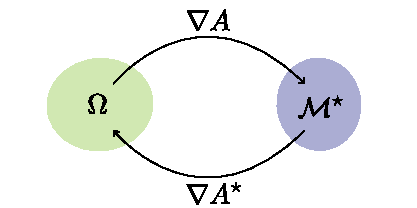
\includegraphics{figures/expf/mapping}
	\caption{\label{bijOmM}Illustration of the bijection between the set of natural parameters $\Omega$ and its image under $\nabla A$, $\mathcal M^{\star}$.}
\end{figure}
%
\subsubsection*{Mean parameter space}
It remains to characterise more precisely the set $\mathcal M^{\star}=\nabla A(\Omega)$. It is a subset of the set of realisable \emph{mean parameters}:\add{notations, set of pdfs in L1}
%
\eqa{
	\mathcal M^{\star} \esp\subseteq\esp \mathcal M &:=& \pab{\mu\in\mathbb R^{d}\mid \exists\, p \in\mathcal P(\mathcal X) \,\,\text{s.t.}\,\, \mu=\E_{p}[\phi(X)] },
}
%
where $\mathcal P(\mathcal X)$ denotes the set of all probability density functions on $\mathcal X$. This space $\mathcal M$ is also known as the \emph{mean parameter space}. It is easy to see that it is convex since $\mathcal P(\mathcal X)$ is trivially convex. More interestingly, it can be shown that, for a minimal exponential family, $\mathcal M^{\star}$ is, in fact, the interior of $\mathcal M$ \citep[theorem 3.3]{wainwright08}. Note that, since the interior of a convex set is necessarily convex, $\mathcal M^{\star}$ is itself convex. Finally, note that since $\mathcal M^{\star}=\mathrm{int}\,(\mathcal M)$, $A^{\star}$ can be continuously extended on $\mathcal M$ by changing the $\max$ in a $\sup$ in \eqref{eq:defconja}. \check{april 17}In a similar fashion, for a point $\mu\in\mathcal M\backslash \mathcal M^{\star}$, we can consider a sequence of points $\mu_{1},\mu_{2},\dots$ in $\mathcal M^{\star}$ such that $\lim_{i\to\infty}\mu_{i}=\mu$ and identify $\nabla A^{\star}(\mu)$ to $\lim_{i\to\infty}\nabla A^{\star}(\mu_{i})$ by continuity. The extended operator is then defined as a mapping from $\mathcal M$ to $\overline\Omega$, the closure of $\Omega$. 
\add{max/sup in notations?, discussion of boundary of Omega for EP when problem in projecting}\check{april 22}



% ====================================
\newpage
\subsection{\label{s:ADF+EP}Assumed density filtering and expectation propagation}
% !TEX root = ../thesis.tex
% -------------------------------------------------------------
\subsubsection{Variational inference in the exponential family}
%
The premises of both ADF and EP is performing variational inference in the exponential family $\mathcal F_{\phi}(\mathcal X)$.\add{check EP/ADF introduced} In the previous point, we showed that a target distribution $p$ could be associated with a point $\mu_p\in\mathcal M$ with $\mu_p=\E_{p}[\phi(X)]$ for a sufficient statistic $\phi$. Further, we showed that if the family is minimal and if $\mu_p\in\mathcal M^{\star}$, the mean parameter could be directly associated to a distribution in $\mathcal F_{\phi}(\mathcal X)$ with parameter $\theta$ given by $\nabla A^{\star}(\mu_p)$. It is therefore natural to consider this distribution $q_{\theta}$ as potentially forming a good approximation to $p$ in $\mathcal F_{\phi}(\mathcal X)$.\check{may15,april24}
%
%\begin{figure}[!h]
%    \center
%	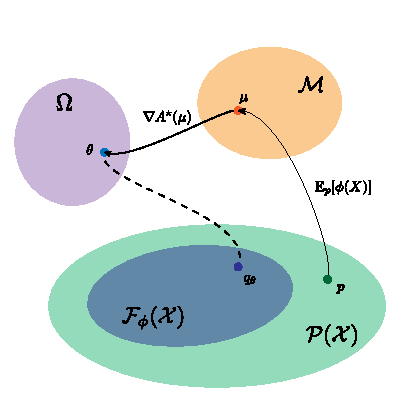
\includegraphics[width=.5\textwidth]{figures/expf/mapping2}
%\caption{blah}
%\end{figure}
This is supported by the fact that this distribution actually minimises the divergence $\KL{p,q_{\theta'}}$. Indeed, observe that
%
\eqa{
	\KL{p,q_{\theta'}} &=& \E_{p}[\log p] - \scal{\theta', \mu_p} + A(\theta'), \label{kldivadf}
}
%
which is a strictly convex function in $\theta'$. By definition, a parameter $\theta=\nabla A^{\star}(\mu_p)$ is such that $\nabla A(\theta)=\mu_p$ and therefore verifies the first order condition. This shows that $q_{\theta}$ minimises the divergence \eqref{kldivadf}. It is useful at this point to define a projection operator $\mathbf P_{\phi}:\mathcal P(\mathcal X) \to \mathrm{cl}(\Omega)$\, with
%
\eqa{	
	\theta \,\,=\,\, \mathbf P_{\phi}[p] &\Longleftrightarrow& \theta \,\,=\,\, \nabla A^{\star}(\E_{p}[\phi(X)]).
}
%
Assuming $\mathbf P_{\phi}[p] \in \Omega$, $q_{\theta}$ is a proper distribution in $\mathcal F_{\phi}(\mathcal X)$ that minimises the KL \eqref{kldivadf} and equivalently verifies the \emph{global moment matching condition} (GMMC) 
%
\eqa{
	(\text{GMMC})\qquad \E_{q_{\theta}}[\phi(X)]&=&\E_{p}[\phi(X)].
\label{eq:GMMC}}
%
It will also be convenient to use the following abuse of notation: for an unnormalised distribution $p_{u}$ with some normalisation constant $Z_{p_{u}}\inv$ we will write $\mathbf P_{\phi}[p_{u}]$ to implicitly mean $\mathbf P_{\phi}[Z_{p_{u}}\inv p_{u}]$.\check{may15,april24}

The application of this projection operator implicitly requires the ability to perform two computations. First, it requires the ability to compute the expected value $\mu_p=\E_{p}[\phi(X)]$ which is typically intractable since we are in a context where we are trying to approximate $p$ for that very purpose. Then, provided we can compute $\mu_p$, we need to be able to apply the inverse mapping $\nabla A^{\star}(\mu_p)$. We will introduce below contexts in which the first requirement can be approximately met. The second requirement effectively means that we are constrained to exponential families for which computing the inverse mapping $\nabla A^{\star}$ can be done explicitly or is cheap to approximate. For continuous state spaces, it is overwhelmingly the Gaussian distribution that is considered in the literature with either a diagonal or a full covariance matrix.\add{probably add a section here on how to compute forward backward operator, maybe put this in appendix. Also cite lots of stuff that uses the Gaussian, if you find anything that doesn't...}\check{may15,april24} 
%
% ----------------------------------------
\subsubsection*{Online Bayesian Learning and Assumed Density Filtering}
%
Let us consider the context of online Bayesian learning where one is interested in the evolution of a posterior distribution $p(x\st y_{1:t})$ given observed \iid\add{notations iid} data points $y_{1:t}$ up to current time $t$ and a new \iid data point $y_{t+1}$. The new posterior is given directly by Bayes rule with $p(x\st y_{1:t+1})\propto p(y_{t+1}\st x) p(x\st y_{1:t})$. In \citet{opper98}, the author considers that the exact posteriors are intractable but suggests constructing a sequence of approximations in the exponential family $\mathcal F_{\phi}(\mathcal X)$. Using the notations from the previous point, the algorithm corresponds to a sequence of iteration of the form
\eqa{	\theta_{t+1} &=& \mathbf P_{\phi}[p(y_{t+1}\st \cdot)q_{\theta_{t}}],	\label{adfonline}}
where, at the first step, $q_{\theta_{0}}$ is replaced by the prior $\pi_{0}$. In words, the posterior up to time $t$ is approximated by the exponential family distribution $q_{\theta_{t}}$ which then serves as prior to form an approximate posterior $p(y_{t+1}\st x)q_{\theta_{t}}(x)$. Given that this approximate posterior is not necessarily in the exponential family, it needs to be projected as per \eqref{adfonline}.\check{april27} At time $t+1$, the distribution $q_{\theta_{t+1}}$ can be now interpreted as an approximation of the posterior distribution given all the data up to that time or 
%
\eqa{	q_{\theta_{t+1}}(x) \esp\approx\esp p(x) &\propto& \pi_{0}(x)\prod_{s=1}^{t+1}p(y_{s}\st x).
}
%
We can therefore reinterpret the algorithm more generally as targeting a distribution $p$ that factorises in a fixed number (say $K$) of factors: 
%
\eqa{
	p(x) & \propto&  \pi_{0}(x)\prod_{i=1}^{K}t_{i}(x) \label{eq:targetfactorises}
}
%
where the factors $t_i$ are nonnegative.\add{notations: make sure it's clear that $\pi_{0}$ is always the prior} This is the \emph{Assumed Density Filtering} algorithm. Note that in this case there is no ``natural ordering'' as in the online learning case and the algorithm can be applied after any permutation of the factors.\check{april27}

\begin{algorithm}[!h]\small
	\caption{\label{alg:adf}\dblue{\emph{\small Assumed Density Filtering}}}
	\begin{algorithmic}[1]
	\State Let $\theta_{1}=\mathbf P_{\phi}[\pi_{0}t_{1}]$
	\For{$i=2:K$}
		\State $\theta_{i}\leftarrow\mathbf P_{\phi}[q_{\theta_{i-1}}t_{i}]$ \Comment{parameter of the new approximation}
%		\State $\omega_{i} \leftarrow \theta_{i}-\theta_{i-1}$\Comment{parameter of the local approximation}
	\EndFor\\
	\Return{$\theta_{K}$}
	\end{algorithmic}
\end{algorithm} 

Let $\omega_{i}=(\theta_{i}-\theta_{i-1})$ denote the difference between subsequent parameters (with $\omega_{1}=\theta_{1}$). Correspondingly $\theta_{K}=\sum_{i=1}^{K}\omega_{i}$, and letting $\tilde t_{i}(x):=\exp\scal{\omega_{i},\phi(x)}$, which can be interpreted as an approximation to the factor $t_{i}$, we can write 
%
\eqa{
	q_{\theta_{K}}(x) &\propto& \pi_{0}(x)\prod_{i=1}^{K}\tilde t_{i}(x).\label{eq:approxadf}
}
% 
The main issue with using ADF on an MRF is that the order in which the graph is read, or equivalently the order in which the factors $t_{i}$ are considered, will affect the final approximation $q_{\theta_{K}}$. A natural extension is therefore to perform multiple passes of ADF while considering random orderings of the factors and correct for the fact that each factor is considered multiple times. This is the core idea behind the \emph{Expectation Propagation} algorithm.\check{may14}
%
% --------------------------------------
\subsubsection*{Expectation Propagation}
%
In the Expectation Propagation algorithm \citep{minka01, minka01b, seeger07, gelman14}, we consider that we have an initial approximation $q_{\theta}\in\mathcal F_{\phi}(\mathcal X)$ that we can write as in \eqref{eq:approxadf} (typically obtained with a pass of ADF) and seek to iteratively improve its parameter $\theta$. At each step, a factor $t_{i}$ is considered and, by contrast to ADF, we now consider the projection $\theta_{i}=\mathbf P_{\phi}[q_{\theta}t_{i}/\tilde t_{i}]$. The difference with ADF is therefore the removal of the previous factor approximation $\tilde t_{i}$ from the current approximation $q_{\theta}$ before the projection. ADF can also be reinterpreted as a single pass of EP where, initially, all the factor approximations are set to $\tilde t_{i}\equiv 1$.\check{may15,april27}

\begin{algorithm}[!h]\small
	\caption{\label{alg:ep}\dblue{\emph{\small Expectation Propagation}}}
	\begin{algorithmic}[1]
	\State Initialise $\theta,\omega_{1},\dots,\omega_{K}$ such that $\theta=\sum_{i=1}^{K}\omega_{i} \in \Omega$ (e.g. via ADF)
	\For{$k=1:N_{\text{EP}}$}
		\State Let $\sigma$ be a random permutation of $(1,\dots,K)$
		\For{$i=1:K$}
    		\State $\theta \leftarrow \mathbf P_{\phi}[q_{\theta^{\text{old}}}t_{\sigma(i)}/\tilde t_{\sigma(i)}]$\Comment{\emph{parameter of the new global approximation}}
    		\State $\omega_{\sigma(i)} \leftarrow \omega_{\sigma(i)} + \theta-\theta^{\text{old}}$\Comment{\emph{parameter of the new factor approximation $\tilde t_{\sigma(i)}$}}
			\State $\theta^{\text{old}} \leftarrow \theta$
		\EndFor
	\EndFor\\	
	\Return{$\theta$}
	\end{algorithmic}
\end{algorithm} 

In Expectation Propagation, we denote by $q_{-i}\propto q_{\theta}/\tilde t_{i}$ a \emph{cavity distribution} and by $q_{i}\propto q_{-i}t_{i}$ a \emph{tilted distribution} \citep{gelman14}. If the EP algorithm converges, then the global parameter $\theta$ is equal to $\mathbf P_\phi[q_i]$ for all $i$ and therefore is such that all the \emph{local moment matching conditions} (LMMC) are met:
%
\eqa{
	(\text{LMMC})\qquad	\E_{q_{i}}[\phi(X)]=\E_{q_{\theta}}[\phi(X)], \quad i=1,\dots,K.\label{eq:LMMC}
} 
%
These conditions can be interpreted as a relaxation of the GMMC \eqref{eq:GMMC} and the EP algorithm can be interpreted as a fixed point algorithm targeting the LMMC.\check{may15}\add{depending on how much you discuss in SNEP, link here to that part and say will discuss in more details.}\add{maybe add ``expectation consistent inference'' the stuff by Heskes etc}


%%%%%%%%%%%%%%%%%%%%%%%%%%%%
\section{Belief Propagation}

\todofr{
    \begin{itemize}\itsep0
    	\item BP on a tree
		\item LBP when iterating
		\item why is it / is it not a good idea (energy min and MERL stuff)
	\end{itemize}
}

% ==================
\section{Discussion}
\todofr{
(see where stuff belongs, either here or in previous points)
\begin{itemize}\itsep0
	\item more literature quotations probably especially indicating the different pieces of work for different applications (?)
	\item can do expoF but in practice people do Gaussian, why
	\item EP energy and showing that it's not really justified, maybe drawing where you show that VB arrives to a point (convergence guarantees, no guarantee of quality), EP goes to a point (no convergence guarantee, no guarantee of quality) and so that we're a bit in the dark. See whether Gelman discusses VB vs EP...
	\item poor recovery of variance, why
	\item link EP, BP, show BP can be interpreted as EP
	\item other, non-KL recovery, make link with choice of loss function in general, discuss that (maybe)
	\item power EP from EP (maybe in SNEP or in EPBP when discussing extensions see how can include story)
	\item comparison VI and MAP (choice of loss function, popularity etc.)
\end{itemize}
}\fi

\chapter[Expectation Propagation for Distributed Bayesian Inference]{\label{chap:EPforDBI}Expectation Propagation for\\ Distributed Bayesian Inference}
\ifsnep% !TEX root = ../thesis.tex

\todofr{
	\begin{itemize}
		\item Geometry and KL and mirror descent
		\item trick of the trade when projections don't work and why
	\end{itemize}
}

\section{Context}
\todofr{
\begin{itemize}
	\item using EP for distributed stuff
	\item SMS (also Turner's work, SEP etc)
	\item 
\end{itemize}
}

\section{The SNEP algorithm}

\section{Comparison of the SNEP and SMS algorithms}

\section{Discussion}\fi

\chapter[Expectation Propagation for Particle Belief Propagation]{\label{chap:EPBP}Expectation Propagation for\\ Particle Belief Propagation}

\ifpbp% !TEX root = ../thesis.tex

In this chapter, we look at ways to implement the loopy belief propagation (LBP) algorithm on an arbitrary MRF with continuous state-spaces. We concentrate in particular on the representation of the messages and the computation of message updates in the LBP algorithm. 

In this chapter, we consider the \emph{nonparametric belief propagation} (NBP) algorithm of \citet{sudderth03} and the \emph{particle belief propagation} algorithm of \citet{ihler09}. We then discuss our \emph{expectation particle belief propagation} (EPBP) algorithm \citep{lienart15} and discuss how it can improve upon both. \check{jul19}

% !!!!!!!!!!!!!!!!!!!!!!!!!!!!!!!!!!!!!!!!!!!!!!!!!!!!!!!!!!!!!!!!!!!!!!!!!!!!!!!!!!!!!!!!!!!!!!!!!!
\section{\label{sec:LBPonCS}Loopy Belief Propagation on Continuous State-Spaces}
At point \ref{point:LBP}, we had shown that, at iteration $n$ of the LBP algorithm, the messages are obtained by computing the following integral:
\eqa{
	m^{n}_{ts}(x_{s}) &=& \int \psi_{st}(x_{s},x_{t})M^{n}_{t s}(x_{t})\dx_{t}\label{eq:mess-update-2}
}
where the pre-messages are given by 
\eqa{
	M_{st}^{n}(x_{s}) &=& \psi_{s}(x_{s}) \prod_{r\in\partial s\backslash t} m^{n-1}_{rs}(x_{s}).
}
Ultimately, we are interested in computing the beliefs obtained by multiplying message and pre-message: $B_{s}^{n}(x_{s}) = m^{n}_{ts}(x_{s})M^{n}_{st}(x_{s})$. There are a few main computational problems to tackle when attempting to run this algorithm in a continuous setting. First, the messages need to be represented in a tractable fashion. Second, the message updates need to be computable and the results easily expressible in the chosen representation system. Lastly, we need to be able to easily compute expected values with respect to the resulting estimators for the beliefs. We discuss below two existing methods attempting to tackle those issues.
%%%%%%%%%%%%%%%%%%%%%%%
\subsection{Nonparametric Belief Propagation}

In \citet{sudderth03}, the authors suggest representing the messages in the LBP iterations as mixtures of Gaussians:
\eqa{	
	\widehat m^{\text{NBP}}_{ts}(x_{s}) &:=& \sum_{i=1}^{M} w_{s}^{i}\,\mathcal N(x_{s};\mu^{i}_{s},\Lambda_{s}). \label{eq:nbp-representation}
}
They call their algorithm \emph{nonparametric belief propagation} (NBP). In order to make computations more efficient, the authors restrict the covariance matrices to be diagonal.
As indicated in the paper, the representation \eqref{eq:nbp-representation} makes sense only when the messages are finitely integrable. To guarantee this, the authors require that all potentials satisfy the following constraints:
\eqa{	
	\sup_{x_{t}} \int \psi_{st}(x_{s},x_{t})\dx_{t} &<&\infty, \quad \text{and}\quad \int \psi_{s}(x_{s})\dx_{s} \esp<\esp \infty,\label{conditions NBP}
}
where the integrals are taken over the range of admissible values for the relevant variable. Provided these assumptions hold, the message updates are well defined and can be explicitly (and efficiently) computed. Computing the beliefs however, requires considering the product of mixtures of $M$ terms leading to a complex representation and an explosion in computational cost. In order to alleviate this, the authors suggest an importance sampling approach targeting the beliefs and fitting mixtures of Gaussians to the resulting weighted particles. 
The computation of the message updates \eqref{eq:mess-update-2} is thereby always done over a constant number of terms.\check{jul19}

\subsubsection*{Main issues}

A key weakness of the NBP algorithm is that the conditions \eqref{conditions NBP} do not hold in a number of important cases (the authors aknowledge this in a footnote of their paper). 
First, the node potentials $\psi_{u}$ are usually proportional to likelihoods of the form $p(y_{u}\st x_{u})$ which need not be integrable in $x_{u}$. In fact, for most non-Gaussian potential, this is the case. Then, there exist applications for which the first integrability condition on edge potentials does not hold. In imaging applications for example, the edge potential can encode a measure of similarity between pixels which need not verify the first integrability condition as in \citet{nikolova00}. Finally, by definition of NBP as an approximated representation with a fixed number of Gaussians, it does lead to consistent estimators of the LBP messages.\check{jul24, jul21, jul19}



%%%%%%%%%%%%%%%%%%%%
\subsection{\label{point:PBP}Particle Belief Propagation}

In \citet{ihler09}, the authors suggest a way to overcome the shortcomings of NBP by considering importance sampling to tackle the update of the LBP messages instead of working with mixtures of Gaussians. For a chosen proposal distribution $q_{u}$ on node $u$ and a draw of $N$ particles $X_{u}^{(i)}\simiid q_{u}$, the messages are represented via an importance sampling estimator of the corresponding integral:
\eqa{		
	&\widehat m_{st}^{\text{PBP}}(x_{t}) 
		:= \sum_{i=1}^{N}w^{(i)}_{st}\psi_{st}(X^{(i)}_{s},x_{t}), \quad\text{where}&	\label{eq:rep-PBP}\\[.4cm]
	&w^{(i)}_{st} 
		\esp\!\propto\esp\! \displaystyle{\widehat M^{\text{PBP}}_{st}(X_{s}^{(i)})\over q_{s}(X_{s}^{(i)})}, \quad\text{and}\quad
	\widehat M^{\text{PBP}}_{st}(x_{s}) \esp\!=\esp\! \psi_{s}(x_{s}) \prod_{r\in\partial s\backslash t} \widehat m^{\text{PBP}}_{rs}(x_{s}).&\nn
}

They call their algorithm \emph{particle belief propagation} (PBP).
This algorithm has the advantage that it does not explicitly require the integrability conditions \eqref{conditions NBP} to hold. 
In terms of choosing proposals, the authors suggest two potential choices: sampling from the local potential $\psi_{s}$, or sampling from the current belief estimate on the node. 
%For the latter, the authors suggest running a short MCMC simulation. \add{explain how they build representation of beliefs}

\subsubsection{Main issue}

The weak point of the PBP algorithm is the choice of proposal distributions.  A poor choice will lead to poor estimators of the messages which, over a few iterations of the LBP algorithm, can lead to poor representations of the beliefs.

The first suggestion by the authors to sample from the local potential is only valid if $\psi_{s}$ is integrable which, as we have mentioned earlier, is not the case in general. The second suggestion implies sampling from a distribution of the form
%
\eqa{		
	\widehat B_{s}^{\text{PBP}}(x_{s}) 
		&\propto& \psi_{s}(x_{s}) \prod_{r\in\partial s} \widehat m^{\text{PBP}}_{rs}(x_{s})	\label{eq:PBP proposal}
}
%
which is a product of mixtures of $N$ components. As in nonparametric BP, naive sampling of the proposal has complexity $\mathcal O {(N^{|\partial {s}|})}$ and is thus, in general, too expensive to consider.

Alternatively the author suggest running a short MCMC simulation targeting it which reduces the complexity to order $\mathcal O {(|\partial {s}|N^{2})}$. Indeed, each MCMC iteration requires evaluating $\widehat B_{s}^{\text{PBP}}$ point-wise which has complexity $\mathcal O {(|\partial{s}|N)}$, and we need at least $\mathcal{O}(N)$ iterations of the MCMC simulation to produce the samples. Note that it is unclear how many more iterations are necessary to get $N$ \emph{good} samples. Running a short MCMC chain (to reduce computational cost) will therefore almost certainly lead to biased samples. In the code the authors shared with us, they run $N$ parallel random walk Metropolis-Hastings chains \citep[chapter 6]{robert04} for a fixed number of steps. This choice may have been motivated by a desire to control the complexity of the algorithm more accurately but it is at the expense of the quality of the samples obtained.

%%%%%%%%%%%%%%%%%%%%%%%%
\section{\label{sec:EPBP}Expectation Particle Belief Propagation}
As for the PBP algorithm, we consider importance sampling to build particle representations of the messages. In our method, however, we consider a \emph{sequence} of proposal distributions at each node from which one can cheaply sample particles at a given iteration of the LBP algorithm \citep{lienart15}.

The novelty of the approach is to propose a principled and automated way of designing a sequence of proposals in a tractable exponential family using the expectation propagation (EP) algorithm. The resulting method, which we call \emph{Expectation Particle Belief Propagation} (EPBP), does not suffer from the restrictive integrability conditions of the NBP algorithm and sampling is done exactly unlike the PBP algorithm which implies that we obtain consistent estimators of the LBP messages.

Further, the development of our method also formally shows that considering proposals close to the beliefs, as suggested by \cite{ihler09}, is a good idea.  Our core observation is that since sampling from a proposal of the form \eqref{eq:PBP proposal} using MCMC simulation is very expensive, we should consider using a more tractable proposal distribution instead. However it is important that the proposal distribution is constructed adaptively, taking into account evidence collected through the message passing itself. We propose to achieve this by using proposal distributions lying in a tractable exponential family, and adapted using EP.

%%%%%%%%%%%%%%%%
\subsection{Proposal selection for PBP}
In this point we discuss the ideal choice of proposal distributions when considering the PBP algorithm. We consider two connected nodes $s$ and $t$ at a a given iteration and assume we have already constructed particle based representations of all incoming messages into both $s$ and $t$ apart from the messages from $s$ to $t$ and from $t$ to $s$. 
We therefore have both pre-messages $\widehat M_{st}$ and $\widehat M_{ts}$ of the form:
%
\eqa{
	\widehat M_{st}(x_{s}) &\propto& \psi_{s}(x_{s}) \prod_{r\in \partial s \backslash t} \widehat m_{rs}(x_{s}).
}
%
This is illustrated in figure \ref{representation-edge-pbp}. 

\begin{figure}[!h]
\center
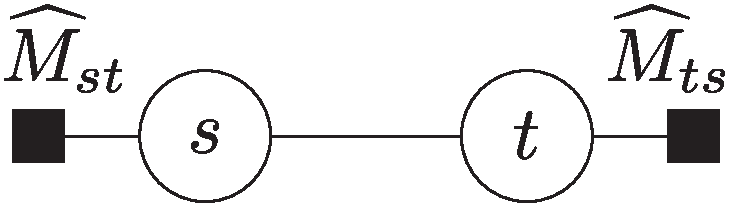
\includegraphics[width=.4\textwidth]{figures/general/belief-st}
\caption{\label{representation-edge-pbp}Illustration of the situation for an edge $(s,t)$: all messages coming into $s$ and $t$ have been approximated apart from the messages between $s$ and $t$. Therefore approximated pre-messages (denoted $\widehat M$) are available on both nodes. We are considering the problem of determining the best proposals on $s$ and $t$ in order to approximate the messages between $s$ and $t$ given the situation.}
\end{figure}

We would like to define $q_{s}$ and $q_{t}$ in a joint manner in such a way that all objects remain consistent with the LBP iterations. For that reason, we consider the joint belief $ B_{st}$ on $s$ and $t$ given the approximation to the pre-messages:
%
\eqa{	
	 B_{st}(x_{s},x_{t}) &\propto& \widehat M_{st}(x_{s}) \psi_{st}(x_{s},x_{t})\widehat M_{ts}(x_{t}).
}
%
The marginals of the joint belief are of the form
%
\eqa{
	B_{st}(x_{s}) &\propto& \widehat M_{ts}(x_{s}) \int \psi_{st}(x_{s},x_{t}) \widehat M_{ts}(x_{t})\dx_{t}\nn\\
	&\propto & \widehat M_{st}(x_{s}) m_{ts}(x_{s}),
}
%
where $m_{ts}$ is the exact (but intractable) LBP message given the pre-message approximation $\widehat M_{ts}$.
Following our point about defining $q_{s}$ and $q_{t}$ in a joint manner, let us consider $q_{s}q_{t}$ as a proposal for the joint belief $ B_{st}$.
We can then define an empirical distribution for it:
%
\eqa{
	\widehat{B}_{st}(x_{s},x_{t}) &\propto& \sum_{i,j=1}^{N} {\widehat M_{st}(X_{s}^{(i)})\psi_{st}(X_{s}^{(i)},X_{t}^{(j)})\widehat M_{ts}(X_{t}^{(j)}) \over q_{s}(X_{s}^{(i)})q_{t}(X_{t}^{(j)})} \delta_{(X_{s}^{(i)},X_{t}^{(j)})}(x_{s},x_{t}). \label{eq:pbp-particle-joint-belief}
}
%
Marginalising this approximation over $x_{t}$ leads to
%
\eqa{
	\widehat{B}_{st}(x_{s}) &\propto& \sum_{i=1}^{N} {\widehat M_{st}(X_{s}^{(i)}) \widehat { m}_{ts}(X_{s}^{(i)}) \over q_{s}(X_{s}^{(i)})} \delta_{X_{s}^{(i)}}(x_{s}), \label{eq:pbb-particle-joint-belief-marg}
}
%
where $\widehat{m}_{ts}$ is the importance sampling estimator for $ m_{ts}$ using $q_{t}$ as proposal. Of course, marginalising \eqref{eq:pbp-particle-joint-belief} over $x_{s}$ leads to an expression analogous to \eqref{eq:pbb-particle-joint-belief-marg}. Focusing on node $s$, the expression \eqref{eq:pbb-particle-joint-belief-marg} indicate that the proposals should be given by
%
\eqa{
	q_{s}(x_{s}) &\propto& \widehat{M}_{st}(x_{s}) \widehat{m}_{ts}(x_{s}) \esp = \esp \psi_{s}(x_{s}) \prod_{r\in\partial s} \widehat{m}_{rs}(x_{s})
	}
where all $\widehat m_{rs}$ are importance sampling estimators built using the corresponding most recent $q_{r}$ as a proposal. Further, this shows that the proposals on nodes should correspond to the most recent approximation of the belief at that node which aligns with the suggestion in \citet{ihler09}.

%%%%%%%%%%%%%%%%
\subsection{The EPBP algorithm}
As we showed in point \ref{point:PBP}, it is computationally expensive to use the particle approximated node belief as the proposal distribution. 
Our idea is therefore consider an approximation $q_{s}$ drawn from a tractable exponential family $\mathcal F_{\phi}$ with a structure matching that of the belief:
%
\eqa{ 
	q_s(x_s) &\propto& \eta_{\circ s}(x_s) \prod_{r\in\partial s} \eta_{rs}(x_s).
}
%
In the experiments we used a Gaussian family but the algorithm is -- in theory  -- not limited to this choice.
Using the framework of expectation propagation (EP) that we discussed in point \ref{point:EP}, we can iteratively find good proxies to the node belief in the exponential family.

For each $r\in\partial s$, we update the $\eta_{rs}$ following the EP framework. We start by forming the \emph{cavity} $q^{\backslash r}_{s}=q_{s}/\eta_{rs}$ and the corresponding \emph{tilted distribution} proportional to $\widehat m_{rs} q_{s}^{\backslash r}$.  The updated distribution is then the projection of the tilted distribution onto the exponential family manifold:
\eqa{ q_{s} &\leftarrow& \mathbf P_{\phi}[\widehat m_{rs}q_{s}^{\backslash r}],}	
where $\mathbf P_{\phi}$ is the projection operator defined in section \ref{eq:def-proj-operator-ep}. Consequently, the factor $\eta_{rs}$ is updated: $\eta_{rs} \leftarrow  q_{s}/ q_{s}^{\backslash r}$. Note that other projection mechanisms than projecting with respect to the Kullback-Leibler divergence can be considered as well. 

In the algorithm as we have described it so far, the EP steps for each incoming message into $s$ and for the node potential are performed first in order to fit the proposal to the current estimated belief at $s$. Then, this estimated belief is used to draw $N$ particles which can be used to form the particle approximated messages from $s$ to each of its neighbours. 
Alternatively, once each particle approximated message $\widehat{m}_{st}(x_t)$ is formed, we can update their exponential family projections $\eta_{st}(x_t)$ immediately. This is the scheme described in algorithm \ref{alg:epbp-node-update}.

\begin{algorithm}[!h]\small
	\caption{\label{alg:epbp-node-update}\idblue{\small Node update in the EPBP algorithm}}
	\begin{spacing}{1.2}
	\begin{algorithmic}[1]
		\State sample $\{X^{(i)}_{s}\}_{i=1}^{N}\simiid q_{s}$	
		\State evaluate the approximate representation of the belief: $$\widehat B_{s}(X_{s}^{(i)}) = \psi_{s}(X_{s}^{(i)})\prod_{r\in\partial {s}}\widehat m_{rs}(X_{s}^{(i)})$$% $q_{u}(x_{u}^{(i)})$
		\For{$v\in \partial {u}$}
			\State evaluate the approximate representation of the pre-message: $$\widehat M_{st}(X_{s}^{(i)}) :=\widehat B_{s}(X_{s}^{(i)})/\widehat m_{ts}(X_{s}^{(i)})$$
			\State compute the corresponding normalised weights: $$ w_{st}^{(i)}\propto \widehat M_{st}(X_{s}^{(i)})/q_{s}(X_{s}^{(i)})$$
			\State update the estimator of the outgoing message: $$\widehat m_{st}(x_{t})=\sum_{i=1}^{N}w^{(i)}_{st}\psi_{st}(X_{s}^{(i)},x_{v})$$
			\State update $\eta_{\circ t}$ to match the update $q_{t} \leftarrow \mathbf P_{\phi}[\psi_{t}q_{t}/\eta_{\circ t}]$ 
			\State update $\eta_{st}$ to match the update $q_{t}\leftarrow \mathbf P_{\phi}[\widehat m_{st}q_{t}/\eta_{st}]$% and update $\eta_{uv}$ correspondingly %compute the cavity distribution $q^{\backslash u}_{v}\propto q_{v}/\eta_{uv}$, get $\eta^{+}_{uv}$ in the exponential family such that $\eta^{+}_{uv}q_{v}^{\backslash u}$ approximates $\widehat m_{uv}q_{v}^{\backslash u}$, update $q_{v}\propto \eta_{uv}^{+}$ and let $\eta_{uv}\leftarrow \eta_{uv}^{+}$
		\EndFor
	\end{algorithmic}
	\end{spacing}
\end{algorithm}

Note that, in the EP step, if the projection leads to an invalid distribution (e.g., in the Gaussian case, if it leads to an element with negative variance), we simply revert the approximation to its previous value as in \citet{minka01}. %\add{this should be discussed in EP intro}

%%%%%%%%%%%%%%%%%%
\subsection{\label{point:epbp-proj}Projection mechanisms}

In the description above, we used the projection $\mathbf P_{\phi}$ from \ref{eq:def-proj-operator-ep}. 
Computing this projection requires computing the moments of the tilted distribution. 
Since this is usually intractable, we have to resort to numerical quadrature. 
In our scenario the moment computation can be performed crudely on a small number of integration points since it only concerns the updating of the importance sampling proposal. 
Since the dimensionality of the tilted distribution in the EPBP algorithm is typically low, a simple deterministic quadrature rule can be used \citep{davis75}. 

The key desired element for the projection is that the resulting updated proposal distribution captures the support of the current estimator of the belief on the node. Since this is a rather general requirement, the KL-projection $\mathbf P_{\phi}$ does not necessarily lead to the best proposals and in fact may suffer from the fact that we have to compute the projection from the mean-parameter space to the natural parameter space $\nabla A^{\star}$ associated with the exponential family of interest which may be numerically unstable.  
This can be mitigated by damping as described at section \ref{sec:ep-for-dbi} but alternative projection schemes can be tried as well.
In our experiments for example, we tried considering the $q_{s}\in\mathcal F_{\phi}$ obtained by doing a maximum likelihood estimation of the natural parameters based on a small number of evaluation points of the tilted distribution. This proved to work well in practice and can be numerically more stable than the original KL-projection.

%%%%%%%%%%%%%%%%%%%%%%
\subsection{\label{sec:EPBP-compcompl}Computational complexity}
The steps that dominate in terms of computational complexity is the evaluation of the approximate representation of the pre-message.
Since the estimator for the belief is a product of $|\partial s|$ mixtures of $N$ components, evaluating at $N$ sampling points is $\mathcal O(|\partial s|N^{2})$. 
Further, the evaluation of the pre-message requires evaluating the message $\widehat m_{ts}$ at $N$ sampling points. Since $\widehat m_{ts}$ is a mixture of $N$ components, this also has quadratic complexity. The dominating complexity of the EPBP algorithm is therefore $\mathcal O(KEN^{2})$ where $K$ is the number of passes done over the graph, and $E$ is the number of edges in the graph.

This inherent quadratic complexity can be reduced. Indeed, instead of we can follow a method presented in \cite{briers05} to sample from a product of mixtures where one draws, for each mixture $\widehat m_{st}$, a set of $M$ indices $\{i^{\star}_{\ell}\}_{\ell=1}^{M}$ from a multinomial with weights $\{w^{i}_{st}\}_{i=1}^{N}$ and samples from a mixture of the corresponding $M$ terms $\psi^{i^{\star}_{\ell}}_{st}$. 
This reduces the cost of the evaluation of the belief to $\mathcal O(|\partial {s}|MN)$ where $M$ is taken to be sub-quadratic in $N$. 
We show in the next section that this version of the algorithm still compares favourably to the quadratic implementation with $M = \mathcal O(\log N)$. 



%%%%%%%%%%%%%%%%%
%\subsection{EPBP for smoothing} % requires backward sampling.

%%%%%%%%%%%
\section{Experiments}

We investigate the performance of our method on MRFs for two simple graphs. This allows us to compare the performance of EPBP to the performance of PBP in depth. We also illustrate the behaviour of the sub-quadratic version of EPBP. Finally we show that EPBP provides good results in a simple denoising application, an example on which the PBP implementation of \citet{ihler09} would struggle to give results in a reasonable time due to its dimensionality.

\subsection{Grid and tree experiments}
We start by comparing EPBP to PBP as implemented by \citet{ihler09} on a $3\times 3$ grid (see \fig{fig:grids} (left)) with random variables taking values on $\mathbb R$. The node and edge potentials are selected such that the marginals are multimodal, non-Gaussian and skewed with
\eqa{	
	\left\{
		\begin{array}{lcl}
			\psi_{u}(x_{u}) &=& \alpha_{1}\mathcal N(x_{u}-y_{u}; \mu_{1},\sigma_{1})+\alpha_{2}\mathcal G(x_{u}-y_{u};\mu_{2},\beta)\\
			\psi_{uv}(x_{u},x_{v}) &=& \mathcal L(x_{u}-x_{v};\mu_{3},\sigma_{3})
		\end{array}
	\right.
}
%-2, 1, 2, 1.3, 0, 2
where $y_{u}$ denotes the observation at node $u$, $\mathcal N(x;\mu,\sigma)\propto \exp(-x^{2}/2\sigma^{2})$ (density of a Normal distribution), $\mathcal G(x;\mu,\beta)\propto \exp(-[(x-\mu)/\beta+\exp(-(x-\mu)/\beta)])$ (density of a Gumbel distribution) and $\mathcal L(x;\mu,\beta)\propto \exp(-|x-\mu|/\beta)$ (density of a Laplace distribution). The parameters were set in an arbitrary fashion to:
$$ \alpha_{1}=0.6,\,\, \alpha_{2}=0.4,\,\, \mu_{1}=-2,\,\,\mu_{2}=2,\,\,\mu_{3}=0, \,\,\sigma_{1}=1, \,\,\sigma_{2}=2, \,\,\beta=1.3. $$
We compare the two methods after 20 LBP iterations.\footnote{The scheduling used alternates between the classical orderings: top-down-left-right, left-right-top-down, down-up-right-left and right-left-down-up. One ``LBP iteration'' implies that all nodes have been updated once.} 
We then repeated the experiments on a tree with 8 nodes (\fig{fig:grids} (right)) where we know that, at convergence, the beliefs computed using BP are proportional to the true marginals. Again, the node and edge potentials are picked such that the marginals are multimodal with this time
\eqa{	
	\left\{
		\begin{array}{lcl}
			\psi_{u}(x_{u}) &=& \alpha_{1}\mathcal N(x_{u}-y_{u}; \mu_{1},\sigma_{1})+\alpha_{2}\mathcal N(x_{u}-y_{u};1\mu_{2},\sigma_{2})\\
			\psi_{uv}(x_{u},x_{v}) &=& \mathcal L(x_{u}-x_{v};\mu_{3},\sigma_{3})
		\end{array}
	\right.
}
with the parameters also set in an arbitrary fashion to:
$$\alpha_{1}=0.3,\,\,\alpha_{2}=0.7,\,\,\mu_{1}=-2,\,\,\mu_{2}=1,\,\,\mu_{3}=0,\,\,\sigma_{1}=1,\,\,\sigma_{2}=0.5,\,\,\sigma_{3}=1.$$
On this second example, we also considered ``pure EP'' with Gaussians to compare with EPBP and PBP. 


\begin{figure}[!h]
\center
%\vspace*{-.3cm}
	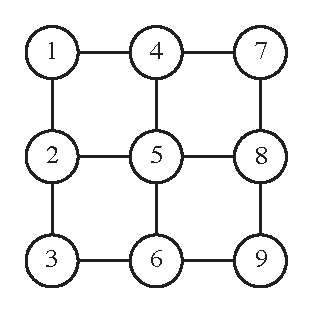
\includegraphics[width=.3\textwidth]{figures/epbp/grid33}
	\hspace*{1cm}
	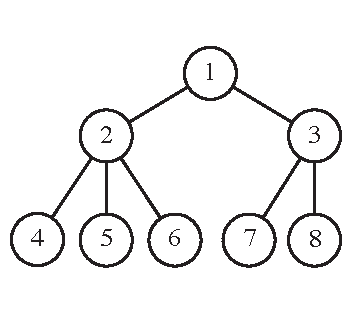
\includegraphics[width=.3\textwidth]{figures/epbp/tree8}
%\vspace*{-.5cm}
	\caption{\label{fig:grids}Illustration of the grid (left) and tree (right) graphs used in the experiments.}
\end{figure}

PBP as presented in \citet{ihler09} is implemented using the same parameters than those in an implementation code provided by the authors: the proposal on each node is the last estimated belief and sampled with a 20-step MCMC chain, the Metropolis Hastings proposal is a normal distribution. For EPBP, the approximation of the messages are Gaussians. The ground truth is approximated by running LBP on a deterministic equally spaced mesh with 200 points. All simulations were run with Julia on a Mac with 2.5 GHz Intel Core i5 processor, our code is available online.\footnote{\url{https://github.com/tlienart/EPBP}.} All the experiments were run multiple times as shown on the figures to account for the inherent stochasticity of the methods. The mean trends are also drawn.
%%%%%%%%%%%%%%%%%%%%%%%%%%%
%\subsubsection{Results of the grid and tree experiments}

The \fig{figCompGrid} compares the performances of both methods. The error is computed as the mean $L^{1}$ error over all nodes between the estimated beliefs and the ground truth. One can observe that not only does PBP perform worse than EPBP but also that the error plateaus with increasing number of samples. This is because the sampling within PBP is done approximately and hence the consistency of the estimators is lost. Note that for EPBP, one observes the expected $1/\sqrt{N}$ convergence of particle methods discussed in \citet{ihler09}.

\begin{figure}[!h]
\center
%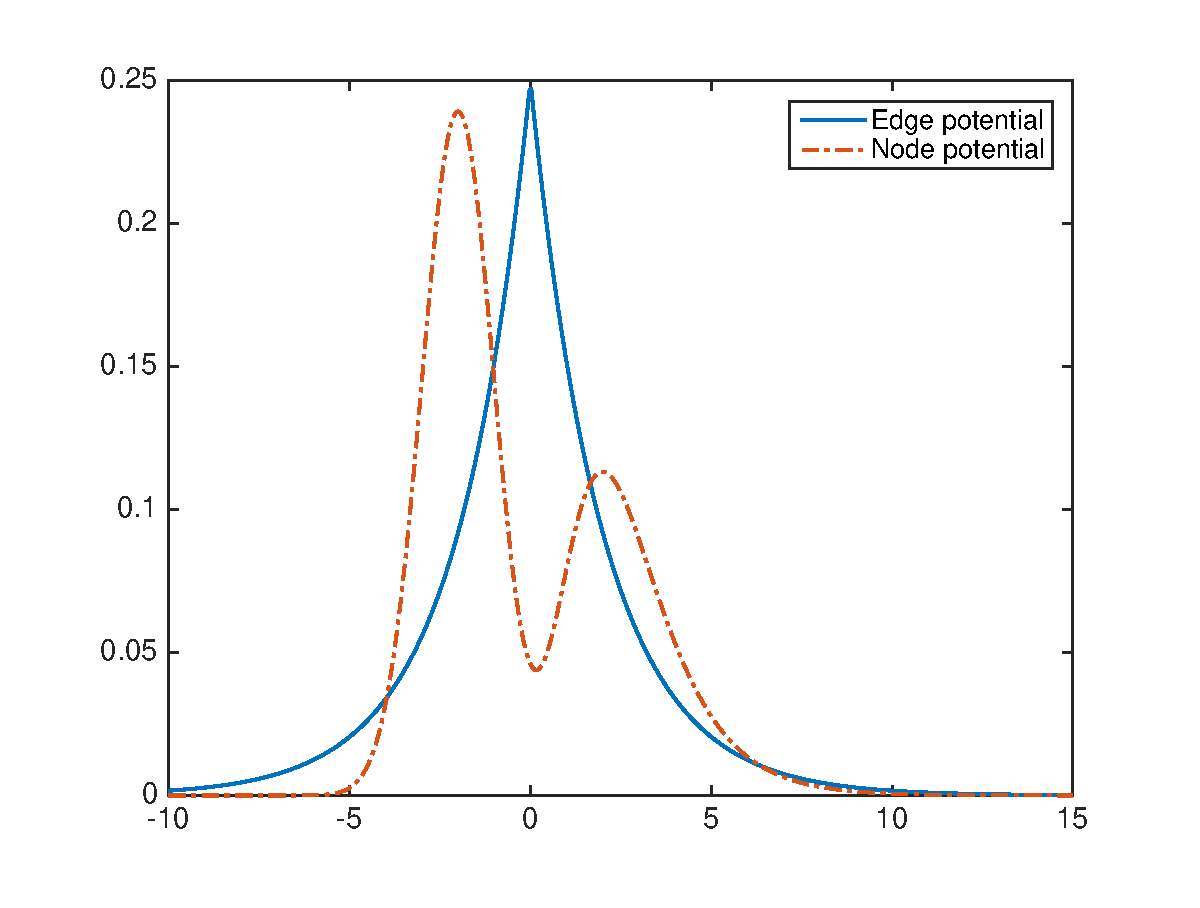
\includegraphics[scale=.25]{figs/node_edge_pot}
%\hspace*{-.6cm}
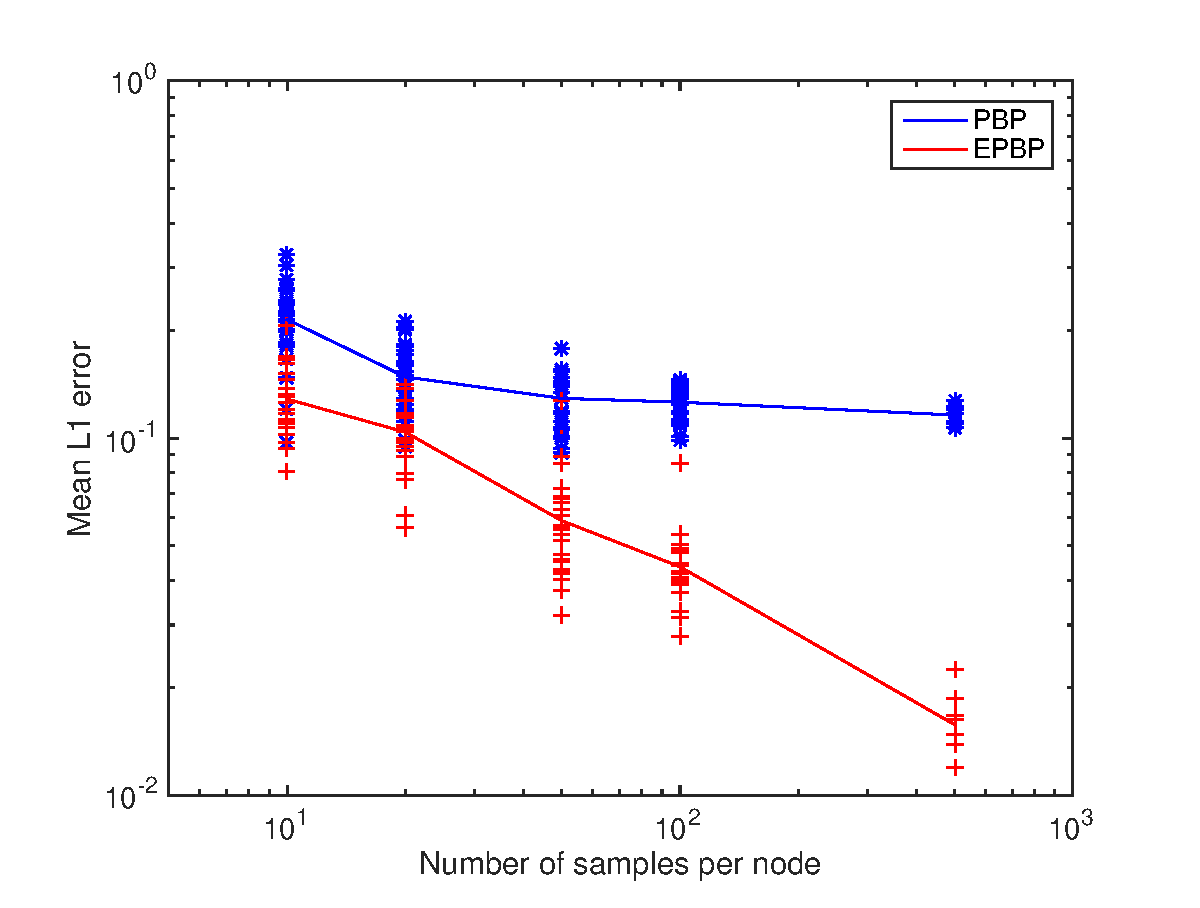
\includegraphics[width=.6\textwidth]{figures/epbp/errComparison}
%\hspace*{-.5cm}
%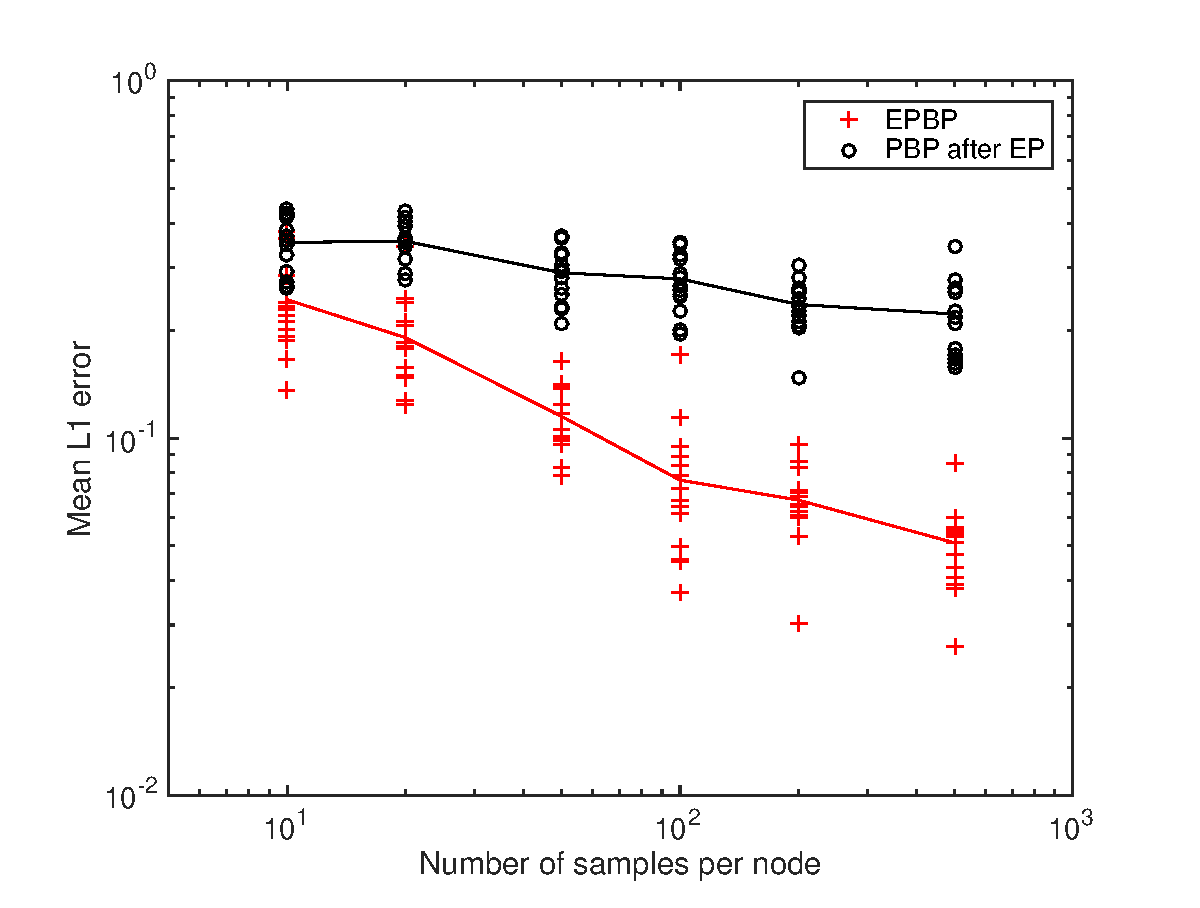
\includegraphics[scale=.35]{figures/epbp/errComparisonEP}
%\vspace*{-.3cm}
\caption{\label{figCompGrid}Comparison of the mean $L^{1}$ error for PBP and EPBP for the $3\times 3$ grid example. EPBP is more accurate for the same number of samples.} %(right) Comparison of the mean $L^{1}$ error for ``PBP after EP'' and EPBP for the tree example. In both cases, EPBP is more accurate for the same number of samples. }
\end{figure}

Figure \ref{compEstBelGrid} compares the estimator of the beliefs obtained by the two methods for three representative nodes (node $1$, $5$ and $9$ as illustrated in \fig{fig:grids} (left)). The figure also illustrates the last proposals constructed with our approach and one can notice that their supports match closely the support of the true beliefs.

\begin{figure}[!h]
%\vspace*{-.5cm}
\center
	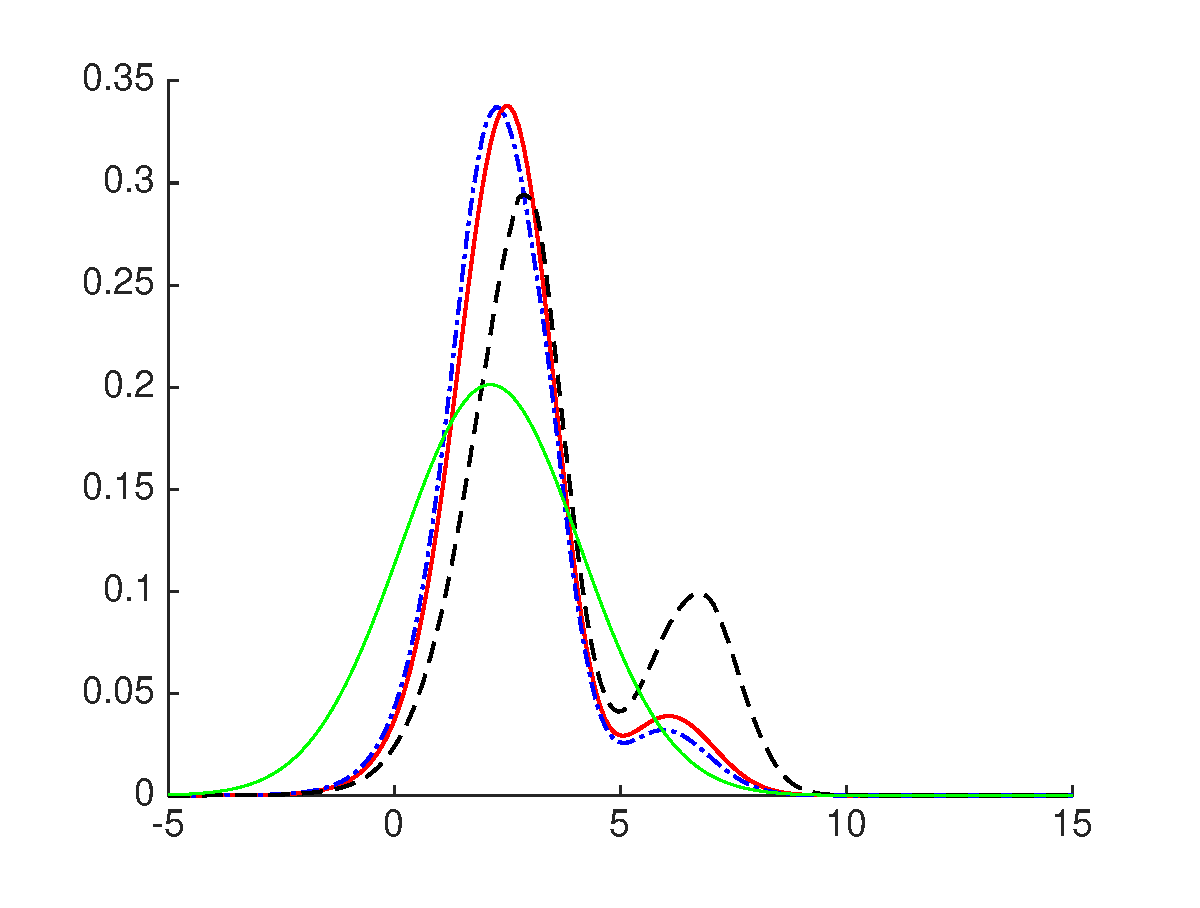
\includegraphics[width=.48\textwidth]{figures/epbp/Gnode1}
	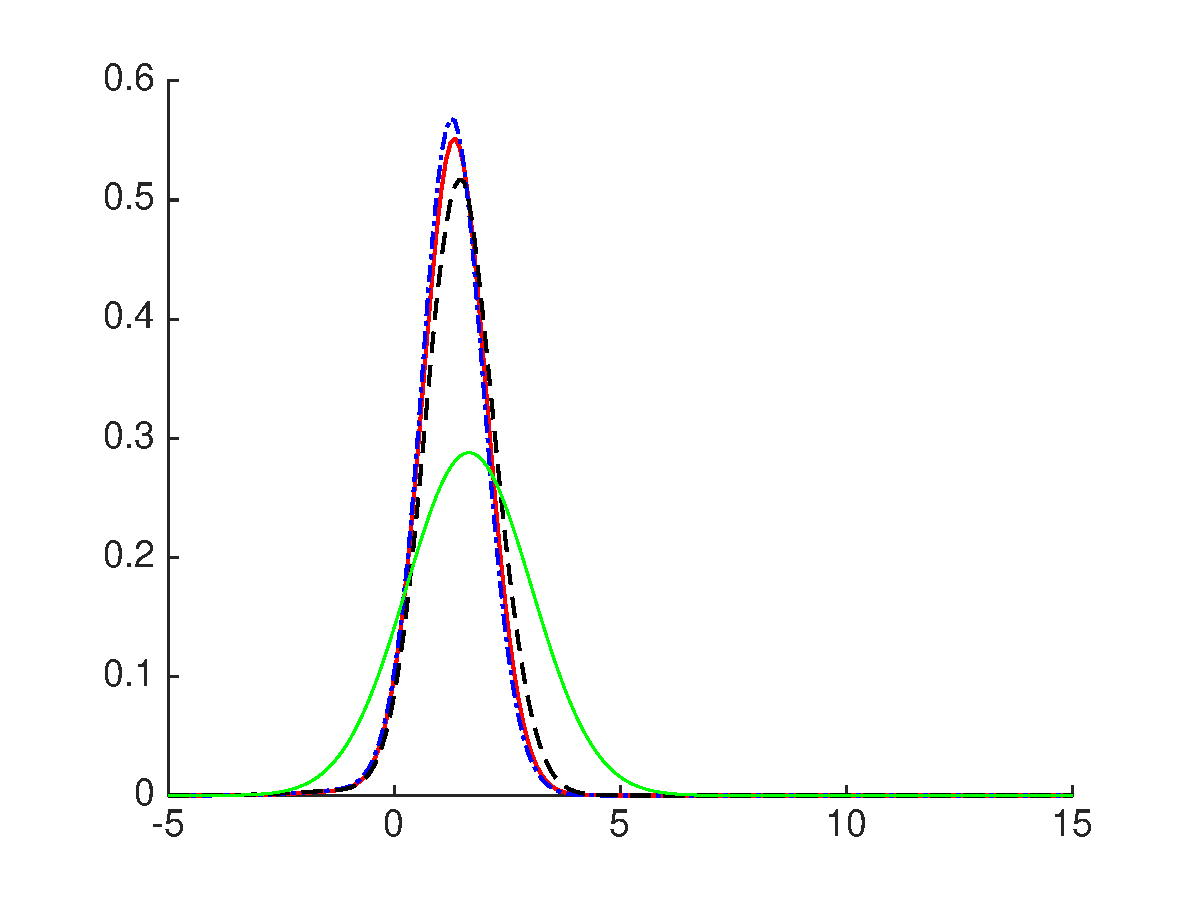
\includegraphics[width=.48\textwidth]{figures/epbp/Gnode5}
	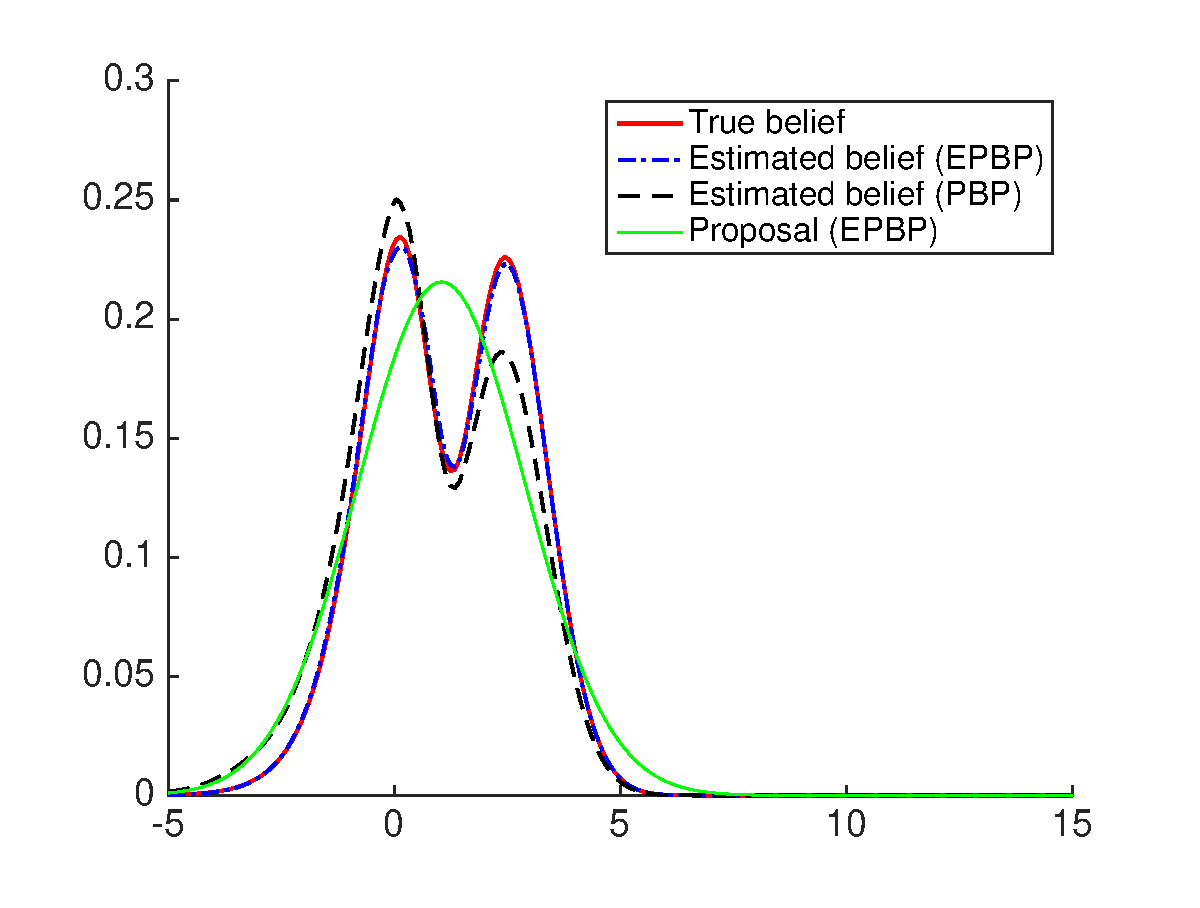
\includegraphics[width=.48\textwidth]{figures/epbp/Gnode9}
%	\vspace*{-.8cm}
%	\hspace*{-.3cm}
%	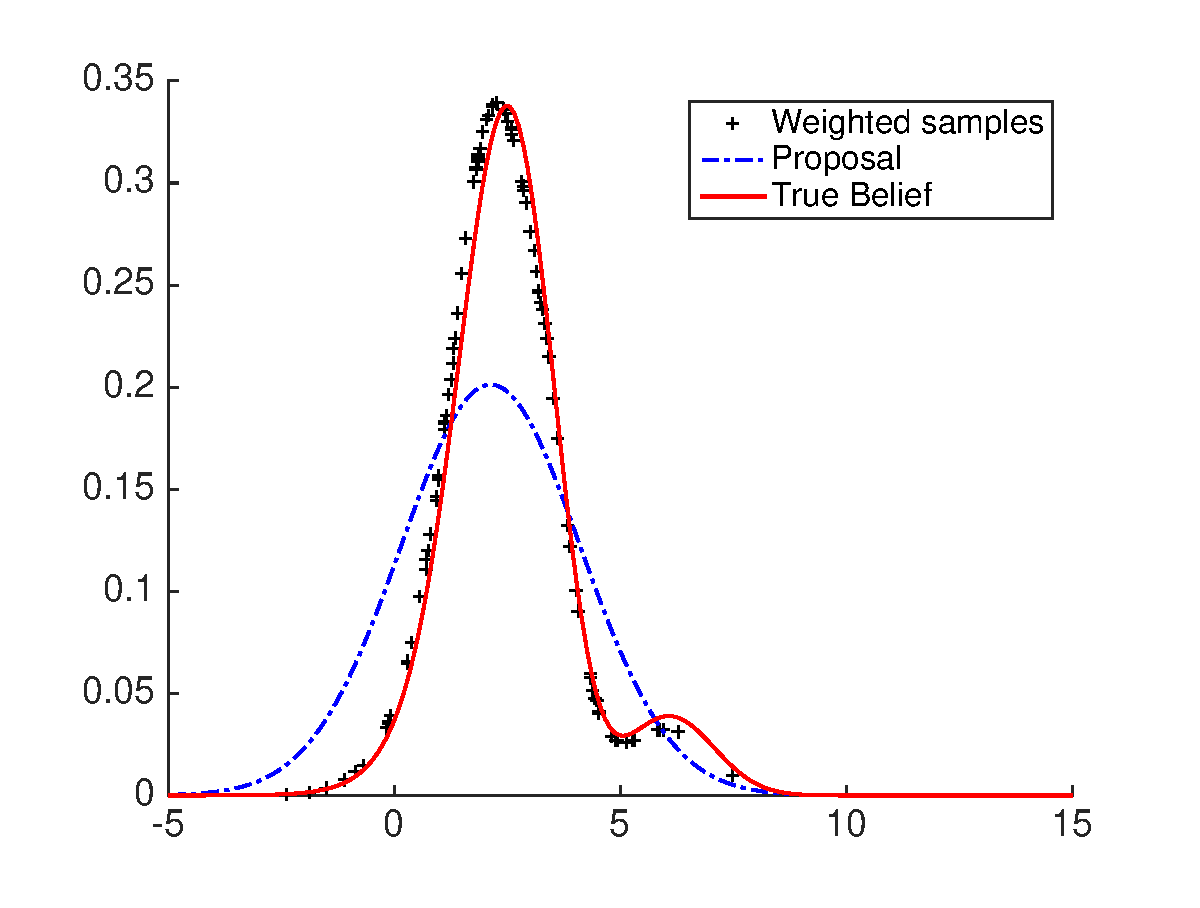
\includegraphics[scale=.25]{figs/node1_epbp}
%	\hspace*{-.5cm}
%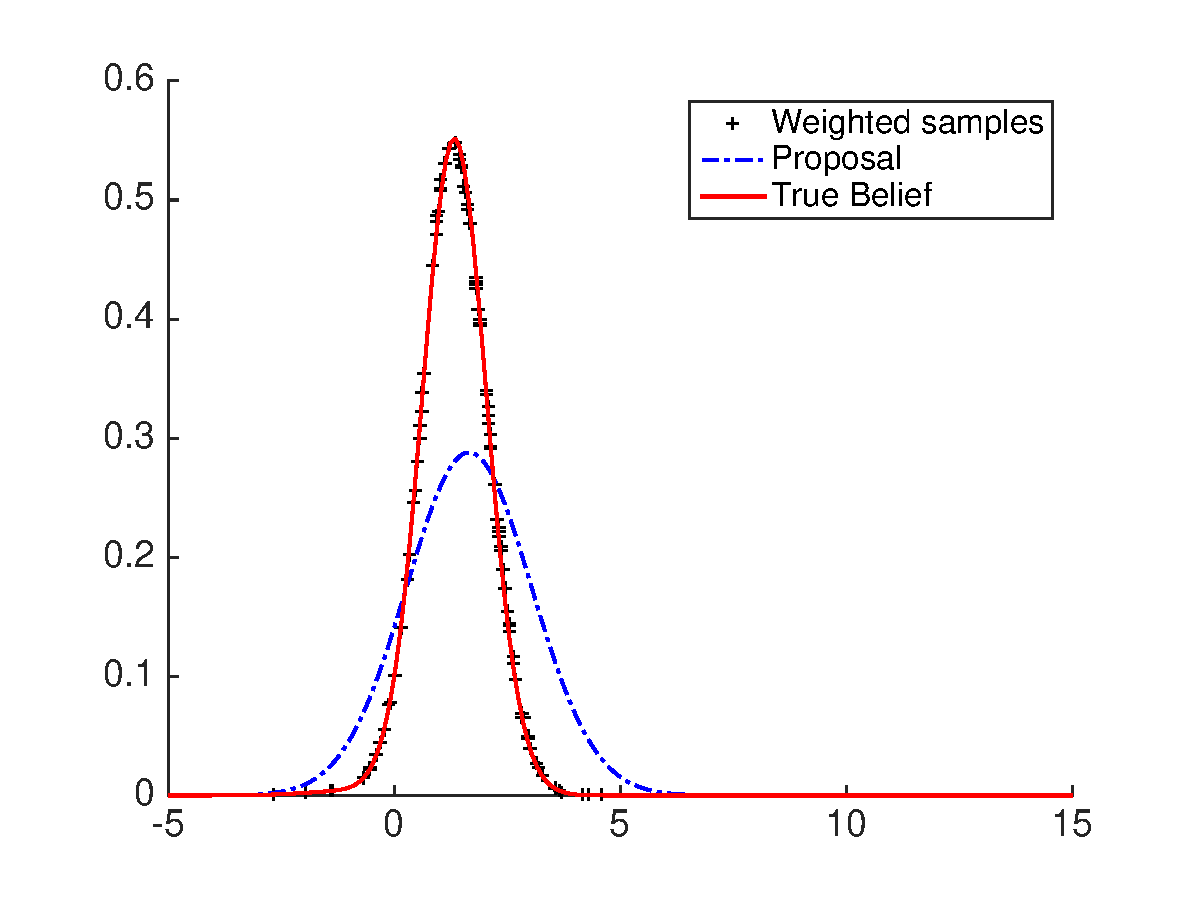
\includegraphics[scale=.25]{figs/node5_epbp}
%	\hspace*{-.5cm}
%	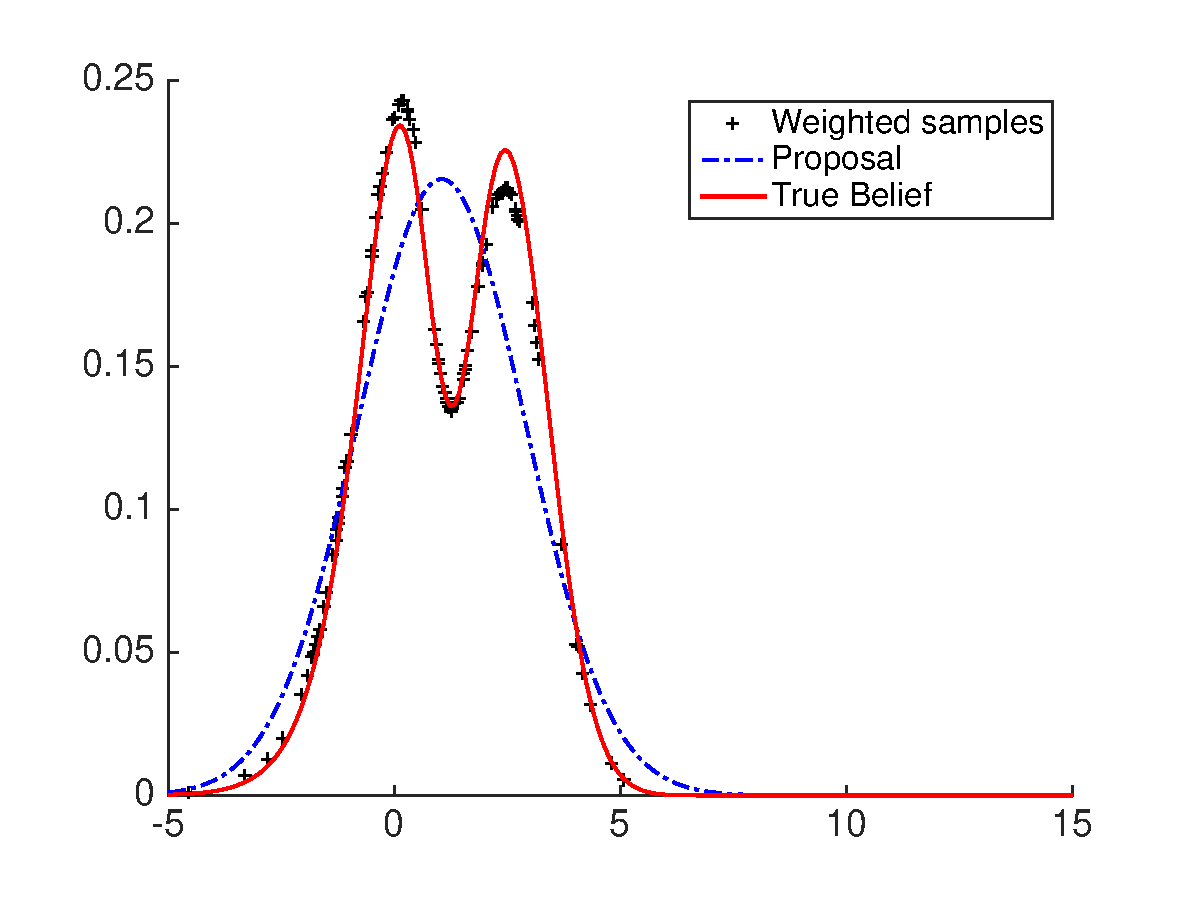
\includegraphics[scale=.25]{figs/node9_epbp}
\caption{\label{compEstBelGrid}Comparison of the beliefs on node $1$, $5$ and $9$ (top left, top right, bottom) as obtained by evaluating LBP on a deterministic mesh (\emph{true belief}), with PBP and with EPBP for the $3\times 3$ grid example. All three plots share the same legend. The proposal used by EPBP in the last step is also illustrated. The results are obtained with $N=100$ samples on each node and $20$ BP iterations. One can observe visually that EPBP outperforms PBP.}
\end{figure}

The speed-up offered by EPBP is very substantial as can be seen in \fig{compConv} (left). Hence, although it would be possible (and sensible) to use more MCMC iterations within PBP to improve its accuracy, it would make the method prohibitively expensive to use compared to EPBP. Figure \ref{compConv} (right) illustrates how the estimated beliefs converge as compared to the true beliefs with increasing number of loopy belief propagation iterations. One can observe that PBP converges more slowly and that the results display more variability which is likely also due to the MCMC runs being too short. %Making them longer is unpractical however as the computational complexity is already higher than that of EPBP.

%
%
%%\newpage
%
%
%
%% THIS IS from THE /DATAMIXNG/ folder

%
\begin{figure}[!h]
\center
%\vspace*{-.5cm}
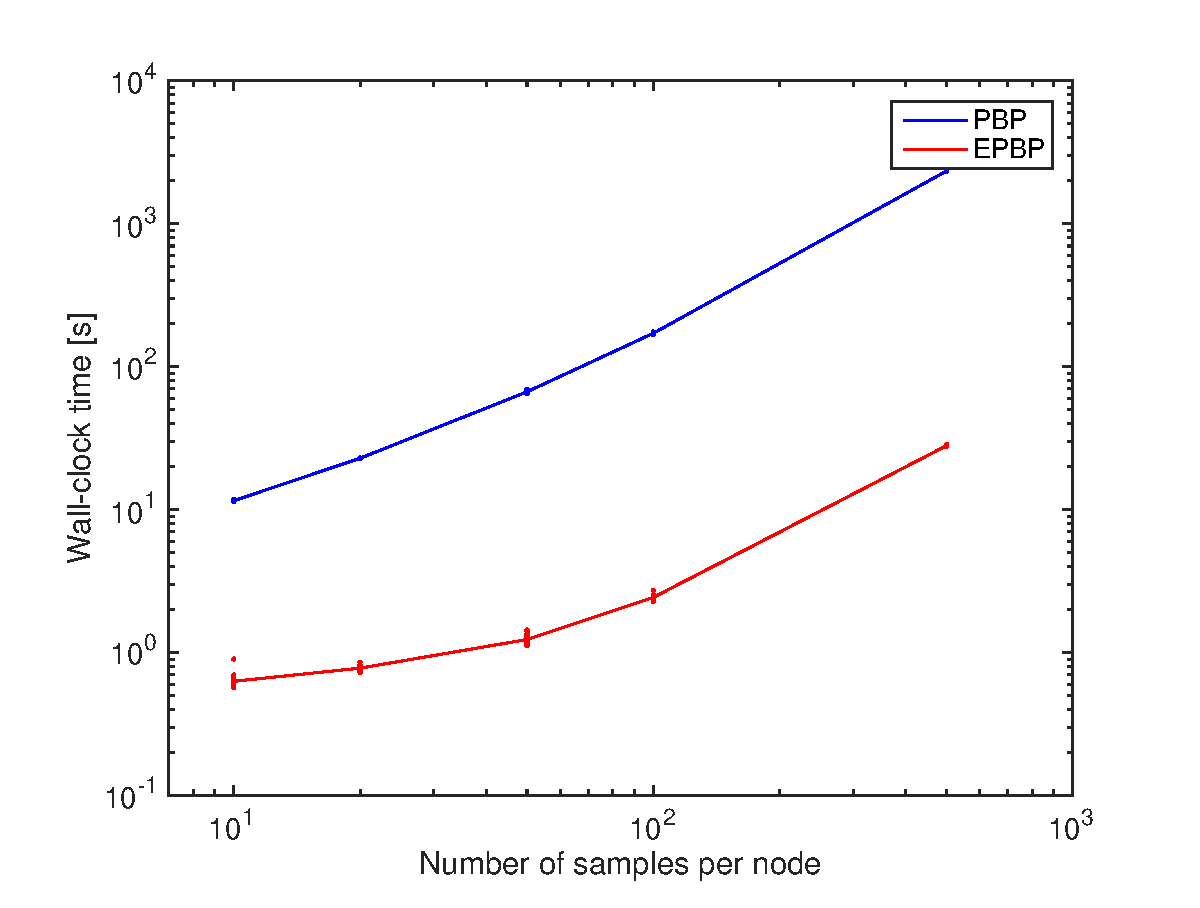
\includegraphics[width=.51\textwidth]{figures/epbp/timeComparison}
\hspace*{-.7cm}
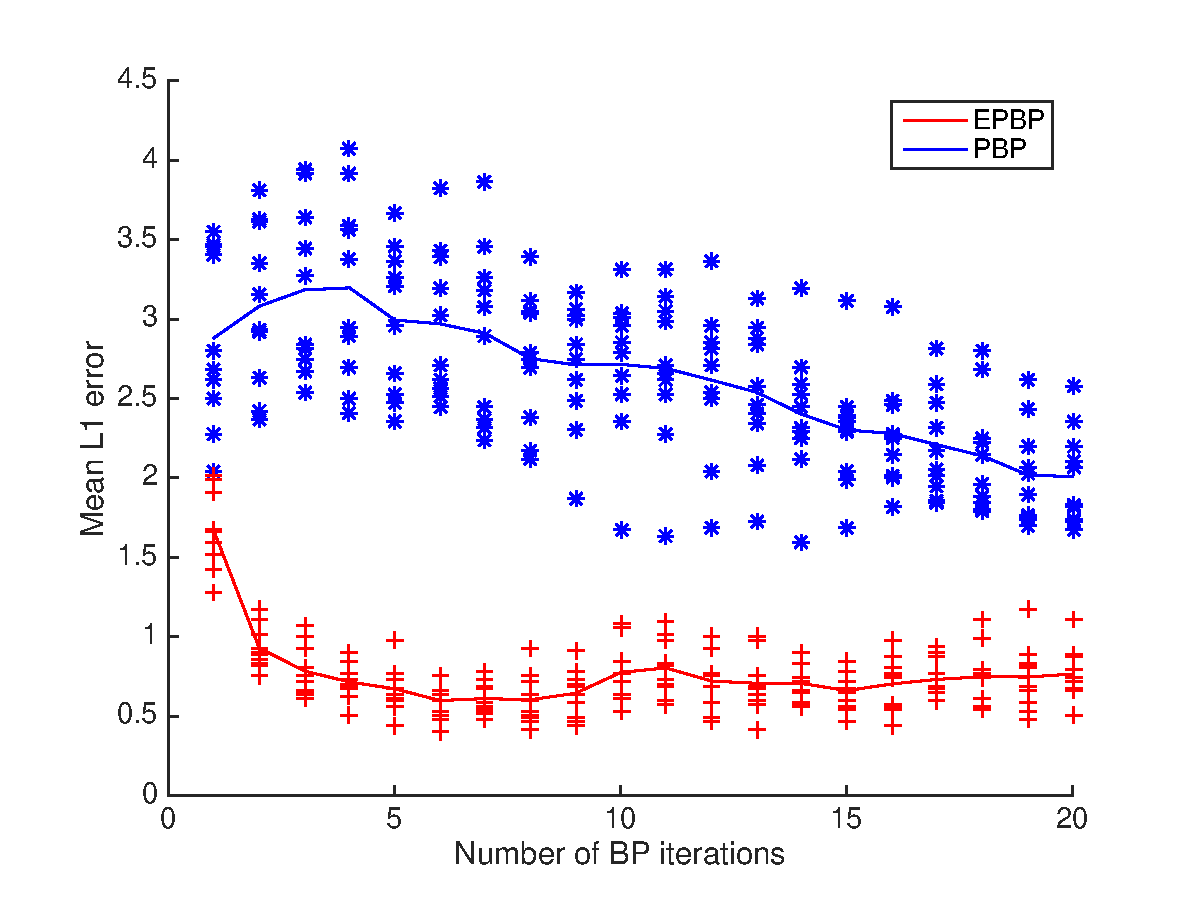
\includegraphics[width=.51\textwidth]{figures/epbp/compBPconv}
%
%\vspace*{-.4cm}
\caption{\label{compConv} (\textbf{left}) Comparison of the wall-clock time needed to perform PBP and EPBP on the $3\times 3$ grid example. (\textbf{right}) Comparison of the convergence in $L^{1}$ error with increasing number of BP iterations for the $3\times 3$ grid when using $N=30$ particles. }%(right) }
\end{figure}
%
%
%\newpage
%
The same experiments were also run on the tree example with similar results.
Additionally, we looked at how ``pure EP'' with normal distributions performs. We also tried using the distributions obtained with EP as proposals for PBP (referred to as ``PBP after EP'' in figures). All those methods underperform compared to EPBP. In particular one can observe in \fig{compPBPaEP} that ``PBP after EP'' converges slower than EPBP with increasing number of samples.
%
%
%
\begin{figure}[!h]
\center
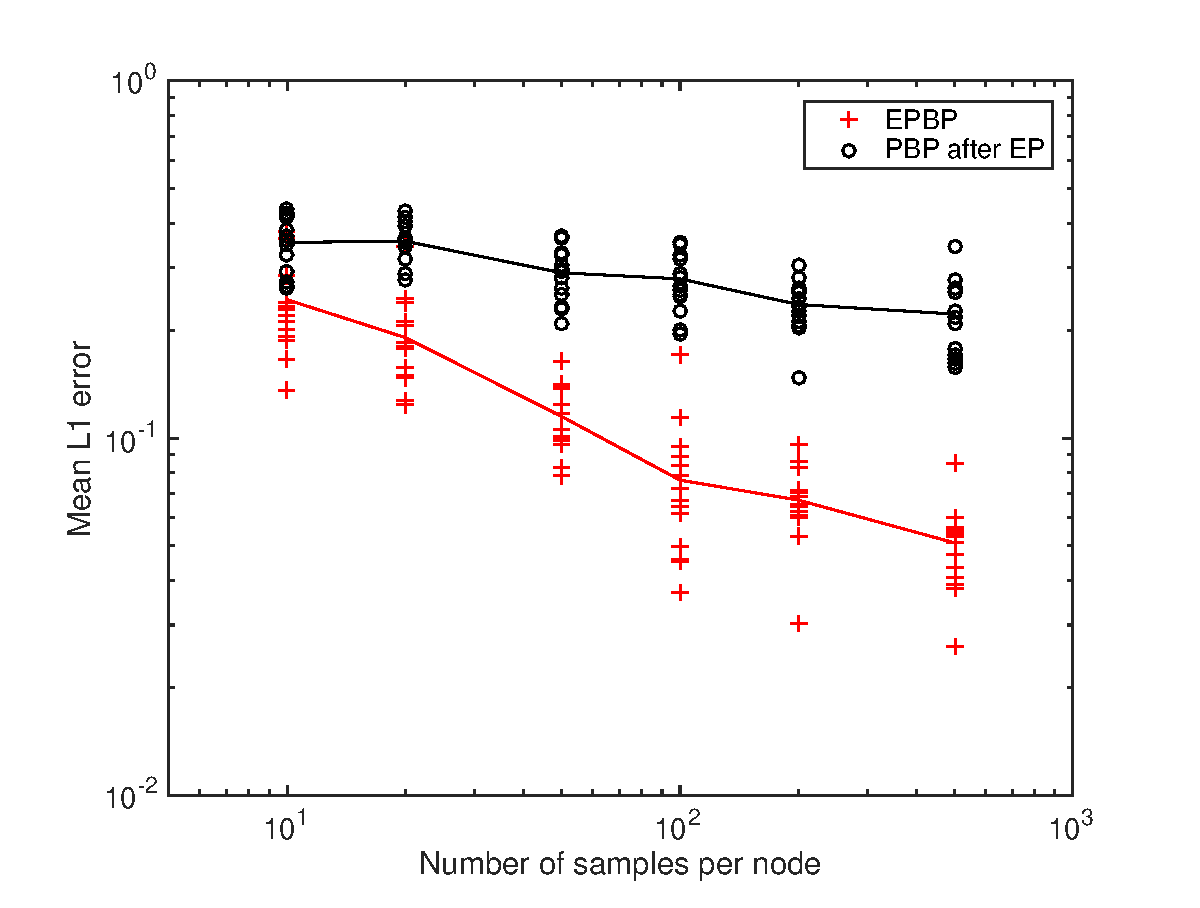
\includegraphics[width=.6\textwidth]{figures/epbp/errComparisonEP}
\caption{\label{compPBPaEP}Comparison of the mean $L^{1}$ error for EPBP and ``PBP after EP'' for the tree example. EPBP is more accurate and converges faster.}
\end{figure}


The \fig{compTree} compares the estimator of the beliefs obtained by all the methods on the tree example for three representative nodes (node $1$, $3$ and $8$ as illustrated in \fig{fig:grids} (right)). As for the grid example, the figure illustrates how EPBP better recovers the true beliefs. 


\begin{figure}[!h]
\center
%\vspace*{-.2cm}
%	\hspace*{-.3cm}
	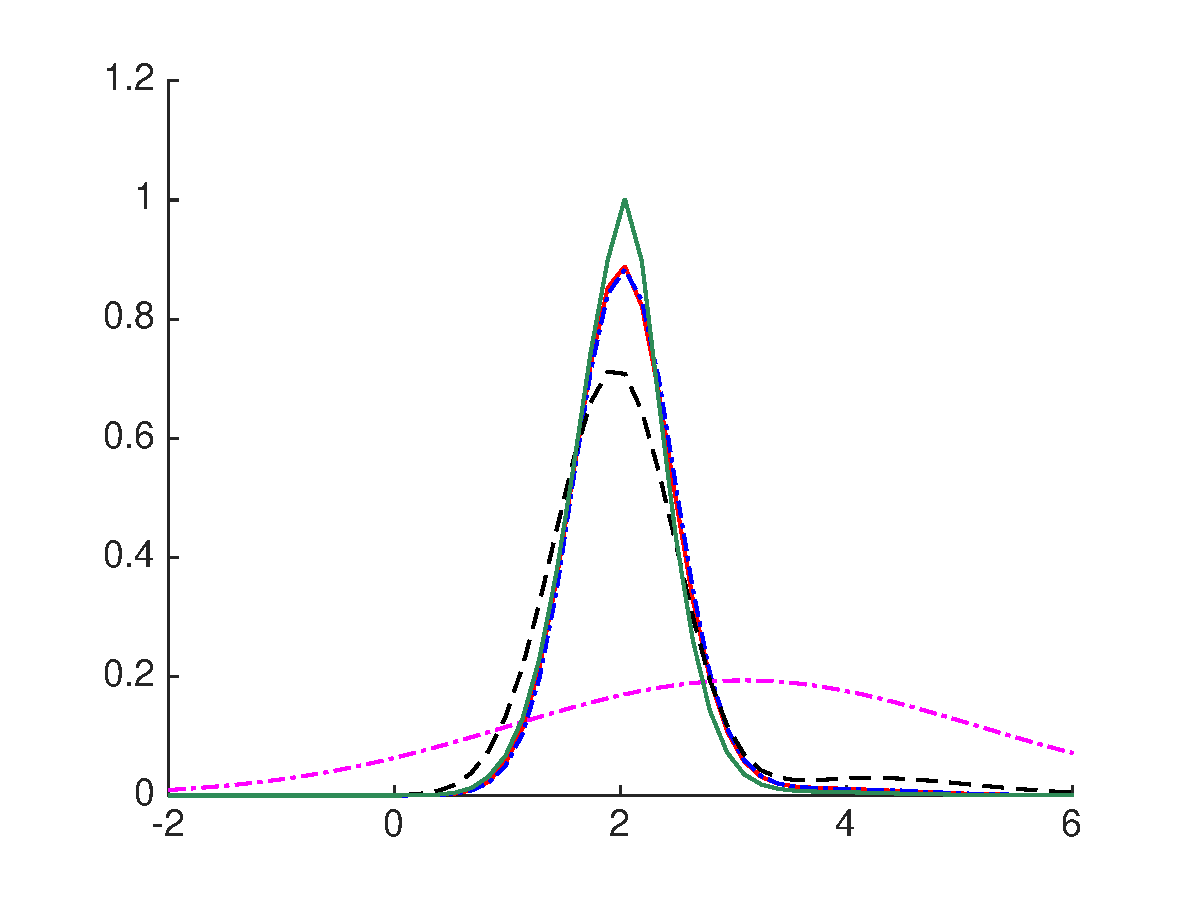
\includegraphics[width=.48\textwidth]{figures/epbp/tree_node1}
%	\hspace*{-.5cm}
	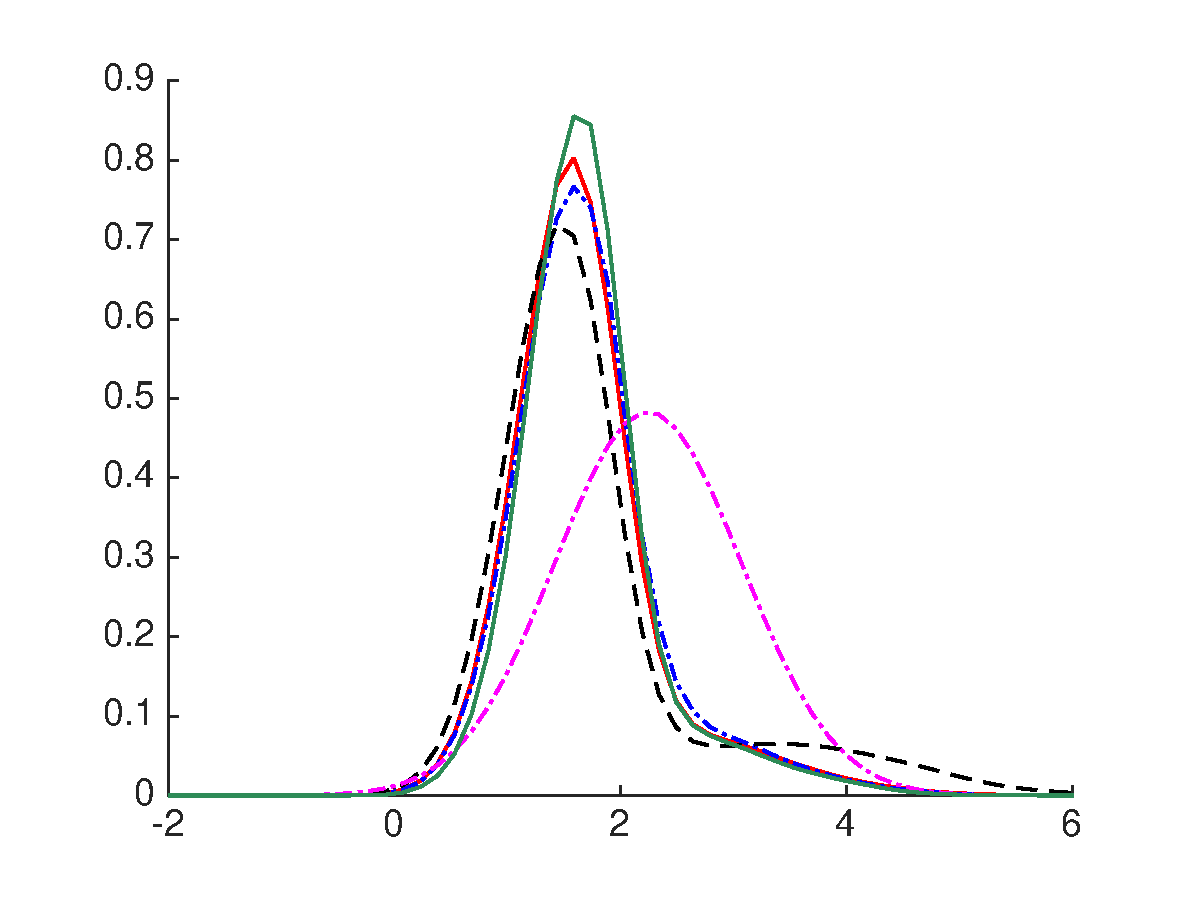
\includegraphics[width=.48\textwidth]{figures/epbp/tree_node3}
%\hspace*{-.5cm}
	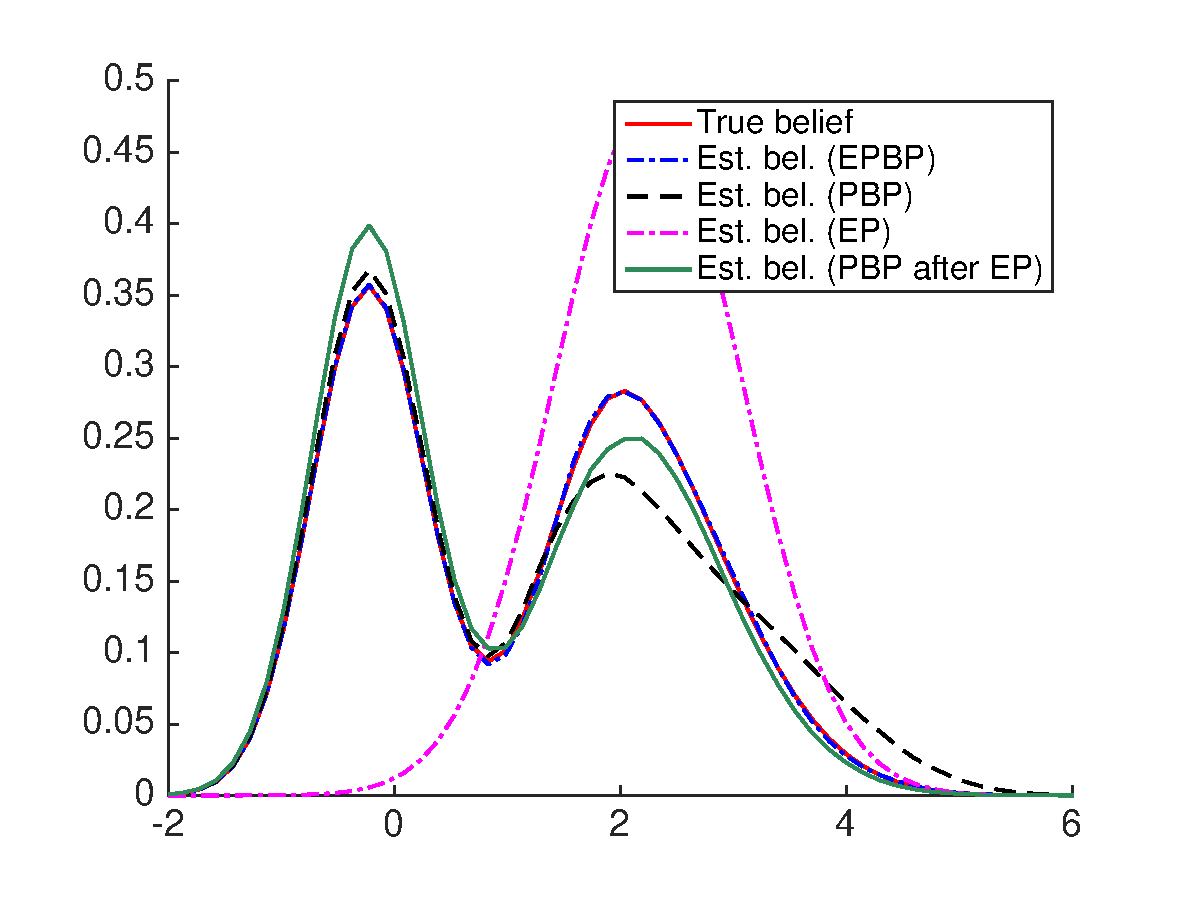
\includegraphics[width=.48\textwidth]{figures/epbp/tree_node8}

	\caption{\label{compTree}Comparison of the beliefs on node $1$, $3$ and $8$ (top left, top right, bottom) as obtained by evaluating LBP on a deterministic mesh, using EPBP, PBP, EP and PBP using the results of EP as proposals. All three plots share the same legend. This is for the tree example with $N=100$ samples on each node and $20$ LBP iterations. Again, one can observe that EPBP outperforms the other methods. }
\end{figure}

\subsection{Sub-quadratic implementation and denoising application}
As outlined at point \ref{sec:EPBP-compcompl}, the inherent quadratic complexity of the EPBP algorithm can be reduced to $\mathcal O(MN)$ where $M$ is the number of mixture components effectively considered to represent the messages. We also consider the maximum likelihood-based projection mechanism as discussed in point \ref{point:epbp-proj} for the two experiments.

We apply this method to the $3\times 3$ grid example in the case where $M=\mathcal O(\log(N))$: for $N=\{10,20,50,100,200,500\}$, we pick $M=\{5, 6,8,10,11,13\}$. The results are illustrated in \fig{figCompNLOGN} where one can see that the $N\log N$ implementation compares very well to the original quadratic implementation at a much reduced cost. 


\begin{figure}[!h]
%\vspace*{-.7cm}
\center
%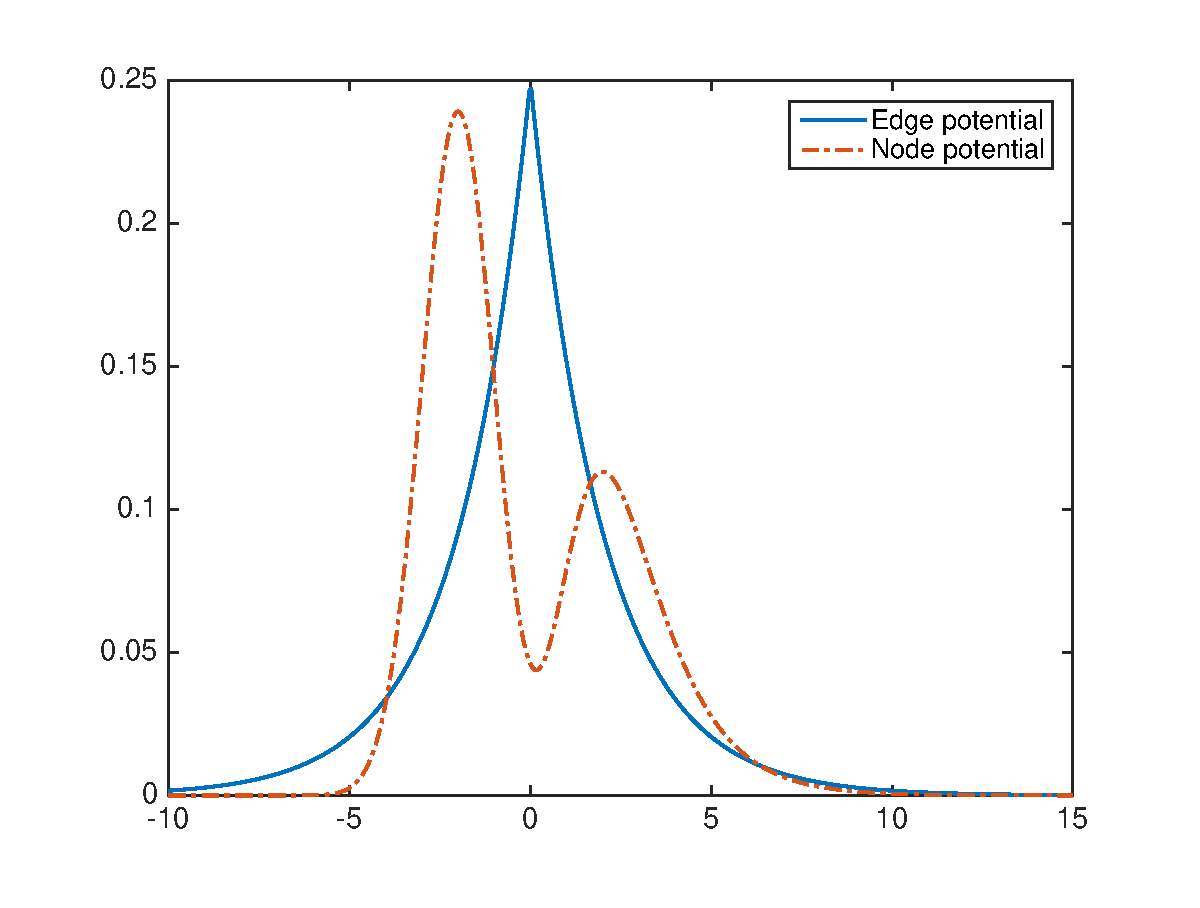
\includegraphics[scale=.25]{figs/node_edge_pot}
%\hspace*{-.6cm}
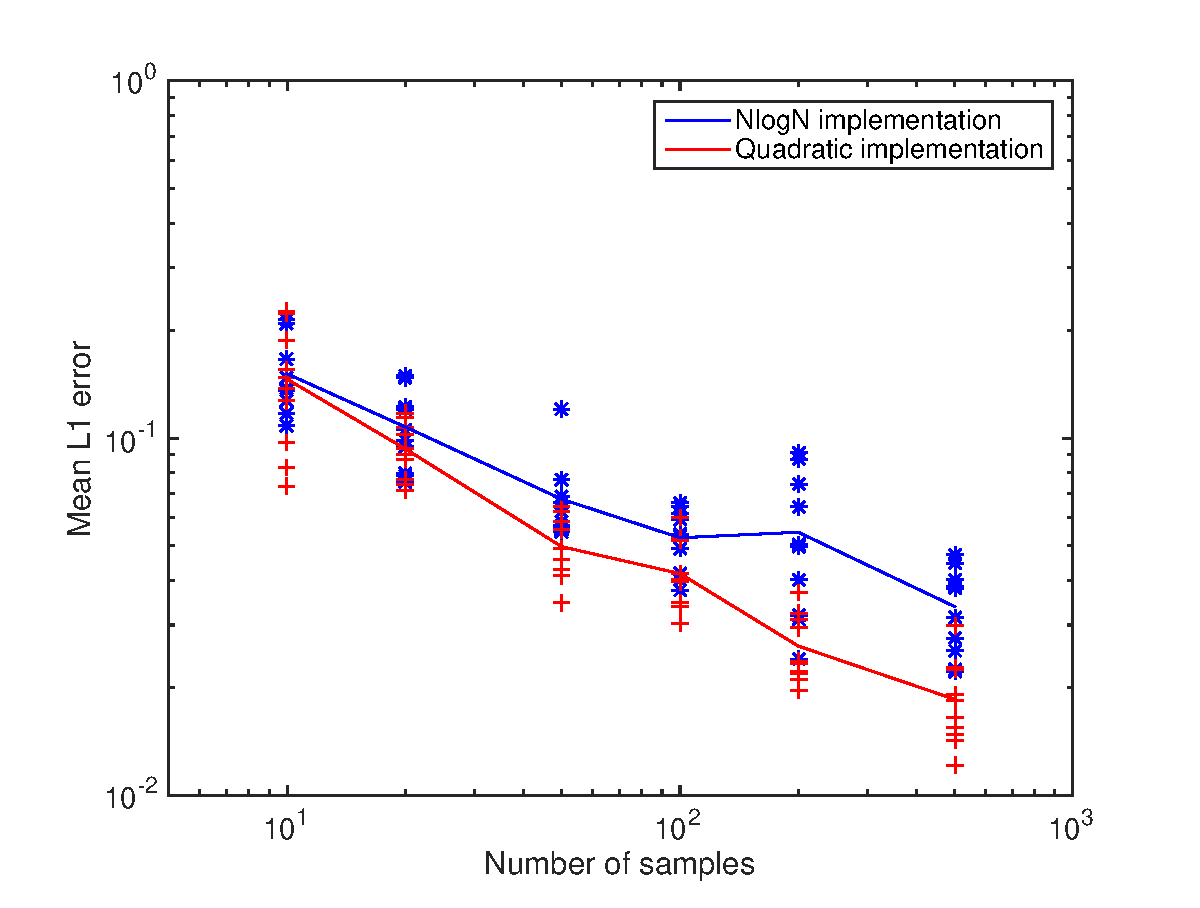
\includegraphics[width=.51\textwidth]{figures/epbp/errCompNLOGN}
\hspace*{-.7cm}
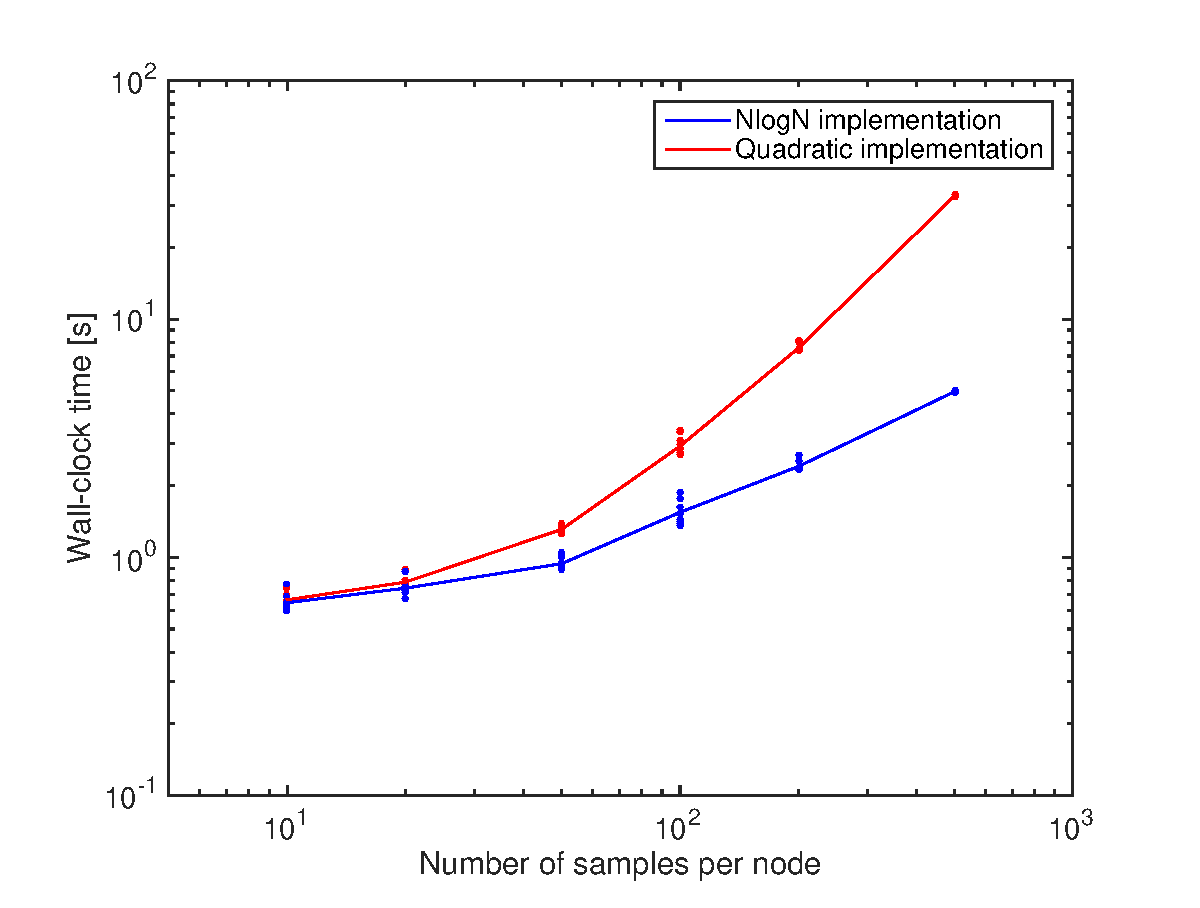
\includegraphics[width=.51\textwidth]{figures/epbp/timeCompNLOGN}
%\vspace*{-.4cm}
\caption{\label{figCompNLOGN}Comparison of the quadratic and $\mathcal O(N log N )$ implementations. (\textbf{left}) Comparison of the mean L1 error, (\textbf{right}) comparison of the wall-clock time. The sub-quadratic implementation performs almost as well as the original implementation and offers a significant speedup.}
\end{figure}


We apply the same sub-quadratic method on a simple probabilistic model for an image denoising problem. The aim of this example is to show that the method can be applied to larger graphs and still provide good results. The model underlined is chosen to showcase the flexibility and applicability of our method in particular when the edge-potential is non-integrable. It is not claimed to be an optimal approach to image denoising.\footnote{In this case in particular, an optimisation-based method such as that of \citet{rudin92} is very likely to yield better results and much faster.}

The node and edge potentials are defined as follows:
\eqa{	
	\left\{
		\begin{array}{lcl}
			\psi_{u}(x_{u}) &=& \mathcal N(x_{u}-y_{u};0,0.1)\\
			\psi_{uv}(x_{u},x_{v}) &=& \mathcal L^{\lambda}(x_{u}-x_{v};0,0.03)
		\end{array}
	\right.,\label{modelIMG}
}
where $\mathcal L^{\lambda}(x;\mu,\beta)=\mathcal L(x;\mu,\beta)$ if $|x|\le \lambda$ and $\mathcal L(\lambda;\mu,\beta)$ otherwise. In this example we set $\lambda=0.2$. The value assigned to each pixel of the reconstruction is the estimated mean of the belief obtained over the corresponding node (figure \ref{figIMG}). The image has size $50\times 50$ (therefore corresponding to a grid graph of 2500 nodes) and the simulation was run with $N=30$ particles per nodes, $M=5$ and $10$ BP iterations taking under 2 minutes to complete with the setup described earlier. 
We compare it with the result obtained with EP on the same model. 
Running PBP or any other quadratic method on this example is prohibitively expensive due to the size of the underlying graph.

\begin{figure}[!h]
\center
%\hspace*{-2cm}
%\vspace*{-.4cm}
\includegraphics[scale=.28]{figures/epbp/denoisingExpleORIG}
\hspace*{.3cm}
\includegraphics[scale=.28]{figures/epbp/denoisingExpleINPUT}
\hspace*{.3cm}
\includegraphics[scale=.28]{figures/epbp/denoisingExpleRECO}
\hspace*{.3cm}
\includegraphics[scale=.28]{figures/epbp/denoisingEP2}
%\hspace*{-1.5cm}
%\vspace*{-.3cm}
\caption{\label{figIMG} From left to right: comparison of the original (first), noisy (second) and recovered image using the sub-quadratic implementation of EPBP (third) and with pure EP (fourth). % with $N=30$ samples per nodes and $10$ BP iterations with the model \eqref{modelIMG}.
}
\end{figure}

% >>>>>>>>>>>>>>>>>>>>>>>>>>>>>>
% >>>>>>>>>>>>>>>>>>>>>>>>>>>>>>
% >>>>>>>>>>>>>>>>>>>>>>>>>>>>>>
% >>>>>>>>>>>>>>>>>>>>>>>>>>>>>>

%%%%%%%%%%
\section{Discussion}

In this chapter, we presented an original way to design adaptively efficient and easy-to-sample-from proposals for a particle implementation of the LBP algorithm. The construction of proposals is done in the Expectation Propagation framework.

We have demonstrated empirically that the resulting algorithm is significantly faster and more accurate than an implementation of the PBP algorithm using the estimated beliefs as proposals and sampling from them using MCMC as proposed in \cite{ihler09}. 
It is also more accurate than using plain EP due to the nonparametric nature of the messages and offers consistent estimators of the LBP messages. 

A sub-quadratic version of the method was also outlined and shown to perform almost as well as the original method on mildly multi-modal models, it was also applied successfully in a simple image denoising example illustrating that the method can be applied on graphical models with thousands of nodes at a reasonable computational cost.

We believe that our method could be applied successfully to a wide range of applications requiring good approximation of the marginals of continuous MRF such as smoothing for Hidden Markov Models \cite{briers10}, tracking or computer vision \cite{sudderth04,felzenszwalb04}. 

%\subsubsection*{Possible paths for future work}

As discussed in point \label{point:epbp-proj}, other projection mechanisms than the KL projection can be considered. We could also look at other discrepancy measure than the KL such as $\alpha$-divergences. This latter choice would suggest considering the power-EP framework \citep{minka04} and could be justified if we seek to build representations of the messages with specific properties. It is unclear to us however how the choice of power in power-EP affects the quality of the proposals representing the node beliefs nor how it would affect the performances of the algorithm.

%To conclude, note that the NBP algorithm of \citet{sudderth03} may in fact be sufficient for a large number of practical applications where MRF does verify the integrability conditions \eqref{conditions NBP} and if the beliefs are not expected to be highly multimodal or non-Gaussian. In a way the NBP algorithm can be compared with the Kalman filter and smoother for a HMM and related techniques: as a first go-to method which may, in fact, lead to satisfactory results. In situations where the NBP algorithm fails or is not applicable, the EPBP algorithm could prove to be a more sensible choice than the PBP algorithm.


\fi


%%%%%%%%%%%%%%%%%%%%
\chapter{Conclusion}

\ifccl% !TEX root = ../thesis.tex

\dred{In this chapter we discuss yada yada avenue of further work, maybe here general conclusion on inference on MRF their relevance etc}
\todofr{ \begin{itemize}
	\item be wary of not introducing new stuff apart from avenues for future work
	\item can discuss here impressions: MRF allow to represent complicated models but the inference is often too slow to be of real practical interests. Approximations exist but often lead to solutions with seemingly insignificant uncertainty estimates. The result is therefore more often of the form of a MAP estimate than anything. In an era of ``big models'' and ``big data'' we therefore question whether it is useful or relevant to attempt using a fully Bayesian model or fake Bayesian models which are actually regularised likelihood models in hiding. While the need for uncertainty estimates is as important as ever for example for automated decision making, it may be better with that regard to attempt using methods which may offer a less aesthetically pleasing theoretical framework than Bayesian statistics but do offer practical and realistic uncertainty estimates for large scale models. A possible avenue for this would be to look at adaptation of the bootstrap methods. This has already been attempted (cite Bags of Little Bootstraps) but can also suffer from dimensionality issues (cite whatever). 
	\item Bayesian inference within a spherical expoF seem particularly naughty and a fake attempt at being bayesian. Very unclear estimates are actually meaningful
	\item Sampling methods are fine but achieving regimes for which the LLN hits is often too expensive leaving us in a realm of models which may work but offer no practical guarantees as to the quality of the estimators. This is particularly the case for big models. Additionally, working with a large number of samples can be numerically challenging.
	\item too little pragmatic literature exists on testing the quality of uncertainty estimates obtained via a sampling or an approximate inference method.
	\item seems to us that it is a \textbf{good} idea to exploit conditional independency structure in a model however it seems to us that the complexity of the computational models attempting to 
\end{itemize}}


\section{On sampling methods}

\section{On approximate inference methods}

\fi

%%%%%%%%%%%


\setcounter{chapter}{0}
\renewcommand{\chaptername}{Paper}
\renewcommand{\thechapter}{\Alph{chapter}}

%\begin*{appendices}
\chapter{Appendix}
% !TEX root = ../thesis.tex

%\todofr{Restructure this part, check appendix command}
%%%%%%%%%%%%%%
\section{\label{app:fearnhead-lg}Fearnhead's Algorithm for a Linear-Gaussian Model }
We describe here an algorithm corresponding to the description in \citep{fearnhead10} with a simple linear and Gaussian underlying dynamic:
%
\eqa{	\syst{
	\pi_{0}(x_1)		&=& \mathcal N(x_1; \mu_0, Q_0) 	\\
	p(x_t\st x_{t-1}) 	&=& \mathcal N(x_t; A_t x_{t-1}, Q)
		}
	\nn}
We start by discussing the form of the normalising densities following the choice suggested in \citep{briers10} and considered in \citep{fearnhead10} then discuss how the corresponding normalised backward information filter (BIF) can be targeted and finally how the particle filter and the normalised BIF can be coupled to yield estimators of the smoothing densities. %\add{code is available in SMC.jl} \check{jul16}
%%%%%%%%%%%%%%%%%%%%%%%%%%%%%
\subsection{\label{app:normalising-density-fearnhead-lg}Normalising densities}
%
The normalising density are defined with $\gamma_{1}\equiv \pi_{0}$ and subsequently 
%
\eqa{
	\gamma_{t}(x_{t}) = \int p(x_{t}\st x_{t-1}) \gamma_{t-1}(x_{t-1})\dx_{t-1}, \quad \text{for $2\le t\le T$}\label{eq-app:propag-fearnhead}
	}
%
The integrand is a product of two Gaussian terms and so clearly $\gamma_{t}$ will be a Gaussian itself. Let $\mu_{t-1}$ and $\Sigma_{t-1}$ denote the mean and covariance matrix of $\gamma_{t-1}$. The quadratic term corresponding to the integrand is (ignoring the constant terms in $x_{t}$ and $x_{t-1}$):\check{jul16,jul11}
%
\eqa{
x_{t}\transp Q\inv x_{t} - 2x_{t}\transp A\transp Q\inv x_{t-1} -2x_{t-1}\transp \Sigma_{t-1}\inv \mu_{t-1} + x_{t-1}\transp A\transp Q\inv A x_{t-1} + \nn\\x_{t-1}\transp \Sigma_{t-1}\inv x_{t-1} - 2\mu_{t-1}\transp\Sigma_{t-1}\inv x_{t-1}.\label{eq-app:initial-quad-term}
}
%
In order for the integral \eqref{eq-app:propag-fearnhead} to simplify, we need to exhibit a Gaussian term in $x_{t-1}$ so that the term integrates out easily. Assembling the terms in $x_{t-1}$ appropriately we get
%
\eqa{
	x_{t-1}\transp (A\transp Q\inv A + \Sigma_{t-1}\inv) x_{t-1} - 2x_{t-1}\transp (A\transp Q\inv x_{t} + \Sigma_{t-1}\inv \mu_{t-1} )\nn.
}
%
In order to form a complete Gaussian, we need to add a term corresponding to the mean. Let us call the mean and covariance matrix of this Gaussian $\mu^{\bullet}_{t-1}$ and $\Sigma^{\bullet}_{t-1}$ respectively. We have:\check{jul16,jul11}
%
\eqa{ \syst{
	(\Sigma^{\bullet}_{t-1})\inv &=& A\transp Q\inv A + \Sigma_{t-1}\inv \\
	(\Sigma^{\bullet}_{t-1})\inv \mu^{\bullet}_{t-1} &=& A\transp Q\inv x_{t} + \Sigma_{t-1}\inv \mu_{t-1}
	}\nn.}
%
The completion term is $\mu^{\bullet}_{t-1}(\Sigma^{\bullet}_{t-1})\inv \mu^{\bullet}_{t-1}$ and must now be removed from the remaining terms in \eqref{eq-app:initial-quad-term} to uncover the resulting Gaussian in $x_{t}$. We finally obtain the following quadratic term in $x_{t}$
%
\eqa{
	x_{t}\transp\pat{Q\inv - Q\inv A \Sigma^{\bullet}_{t-1} A\transp Q\inv}x_{t} - 2x_{t}\pat{ Q\inv A \Sigma^{\bullet}_{t-1} \Sigma\inv_{t-1}\mu_{t-1} }.\nn
}
%
This last expression gives the following recursion for the mean and the covariance matrices of the $\gamma_{t}$ for $t=2,\dots, T$:
%
\eqa{\syst{
	\Sigma_{t}\inv &=& Q\inv - Q\inv A\Sigma^{\bullet}_{t-1}A\transp Q\inv \\	\mu_{t} &=& \Sigma_{t}\pat{ Q\inv A \Sigma^{\bullet}_{t-1} \Sigma\inv_{t-1}\mu_{t-1} }
	}
}
%
%%%%%%%%%%%%%%%
\subsection{Targeting the normalised BIF}
Now that we have defined the normalising densities, we can sample backwards to target the normalised BIF. Let us denote by $\tilde X^{(j)}_{t}$ and $\tilde w^{(j)}_{t}$ the particles and weights associated with the normalised BIF. The initial set of particles for step $T$ can be sampled from the optimal proposal $\gamma_{T}(x_{t})p(y_{T}\st x_{T})$ which is a Gaussian in $x_{T}$; using a similar approach than in the previous point, it is easy to see that the mean $\tilde \mu_{T}$ and covariance matrix $\tilde \Sigma_{T}$ are given by\check{jul16}
%
\eqa{\syst{
	\tilde\Sigma_{T}\inv &=& \Sigma_{T}\inv + B\transp R\inv B\\
	\tilde\mu_{T} &=& \Sigma_{T}\pat{\Sigma_{T}\inv \mu_{T} + B\transp R\inv y_{T}}
}\nn
}
The weights are uniform since the sampling is done from the optimal proposal. Subsequently, the optimal proposal for the following steps is derived from \eqref{recursion joint BIF}:
%
\eqa{
	q(x_{t}\st \tilde X^{(j)}_{t+1}) &=& {\gamma_{t}(x_{t})p(x_{t+1}\st x_{t}) p(y_{t}\st x_{t}) \over \gamma_{t+1}(\tilde X^{(j)}_{t+1})},\nn
}
%
and the numerator is a Gaussian in $x_{t}$ and, again, it is easy to obtain
%
\eqa{\syst{
	\tilde\Sigma_{t}\inv &=& \Sigma_{t}\inv + B\transp R\inv B + A\transp Q\inv A\\
	\tilde\mu_{t} &=& \Sigma_{t}\pat{\Sigma_{t}\inv \mu_{t} + B\transp R\inv y_{t}+A\transp Q\inv x_{t+1}}
	}\nn}
%
This time, the weights need to be adapted to reflect the term $\gamma_{t+1}(\tilde X^{(j)}_{t+1})$ which is easily computed as it is the likelihood of a Gaussian with known mean and variance. Therefore, we have for $t=T-1,\dots,1$:
%
\eqa{\syst{
	\tilde X^{(j)}_{t} &\sim & \mathcal N(x_{t}; \tilde\mu_{t}, \tilde \Sigma_{t})\\
	\tilde w^{(j)}_{t} &\propto& \tilde w^{(j)}_{t+1}/\gamma(\tilde X^{(j)}_{t+1}) 
}\quad \text{for $j=1,\dots,N$}.\nn
}
%
\subsection{Targeting the smoothing distributions}
The last step of the algorithm is the combination of the representation of the predictive density relying on a particle representation of the filtering densities $\{X^{(i)}_{t}, w^{(i)}_{t}\}_{i,t=1}^{N,T}$ with that of the normalised BIF. For this, as suggested in \citet{fearnhead10}, we follow the procedure below:
%
\eqa{\syst{ i^{\star} & \sim&\mathcal M(\{w^{(i)}_{t}\}_{i=1}^{N}) \\
		 j^{\star} & \sim&\mathcal M(\{\tilde w^{(j)}_{t}\}_{i=1}^{N})\\
		 \overline X^{(j)}_{t} &\sim& \varphi_{i^{\star},j^{\star}}(x_{t})
} \quad\text{for $j=1,\dots,N$, and $t=1,\dots,T$}\nn
}
%
where $\varphi_{i^{\star},j^{\star}}(x_{t}) = p(\tilde X^{(j^{\star})}_{t+1}\st x_{t})p(y_{t}\st x_t)p(x_{t}\st X^{(i^{\star})}_{t-1})$ and no reweighing step is needed since we can sample from it exactly (it is a Gaussian) and it is the optimal proposal. Using the same approach as in the previous two points, if we denote the parameters of the optimal proposal $\varphi_{i^{\star},j^{\star}}$ as $\overline \mu_{t}$ and $\overline \Sigma_{t}$ then:\check{jul16}
%
\eqa{\syst{
	\overline\Sigma\inv_{t} &=& Q\inv+ A\transp Q\inv A + B\transp R\inv B\\
	\overline\mu_{t} &=& \overline\Sigma_{t}\pat{A\transp Q\inv \tilde X^{(j^{\star})}_{t+1} + Q\inv A X^{(i^{\star})}_{t-1} + B\transp R\inv y_{t} }
}\nn
}
%











% !TEX root = ../thesis.tex

\section{\label{app:MDA+NG}Mirror Descent and Natural Gradient}

In this part we show briefly the reasoning behind the mirror-descent algorithm focusing on the case of the KL geometry that is considered in the core document.

\subsection{Classical gradient descent}
We start from the generic problem of unconstrained minimisation of a convex function $f$. Additionally, we assume that the function has a computable gradient $\nabla f$ everywhere. The gradient descent algorithm considers the following iterative scheme:
\eqa{		x_{k+1} &=& x_{k} - \alpha_{k}\nabla f(x_{k}),	\nn}
which, under some conditions on the sequence of step-sizes $(\alpha_{k})_{0}^{\infty}$ will converge to a minimiser of the function i.e., an $x^{\star}$ such that $f(x^{\star})\le f(x)$ for all $x$. This scheme is equivalent to solving a sequence of optimisation problems:
\eqa{		x_{k+1} &=& \arg\min_{x}\quad\pab{\scal{x,\nabla f(x_{k})} + {1\over \alpha_{k}}{\bnorm{x-x_{k}}^{2}\over 2}  }. 	}
This re-formulation shows that the gradient-descent is explicitly linked to an isotropic Euclidean geometry via the distance $d(x,y)=\bnorm{x-y}^{2}/2$. Other geometries can be considered by considering other distances or divergences. In particular, when a Bregman divergence is considered we get the mirror descent algorithm as shown below.

\subsection{Bregman divergences}
Consider a smooth, strictly convex function $\varphi$. By definition, this function is such that for any couple of points $(x,z)$ in its domain with $x\neq z$, 
\eqa{		\varphi(z) &>& \varphi(x) + \scal{z-x,\nabla \varphi(x)}.\nn	}
We can therefore build a divergence by rearranging the previous inequality:
\eqa{		B_{\varphi}(z,x) &:=& \varphi(z)-\varphi(x)-\scal{z-x,\nabla \varphi(x)}.	}
Note that $B_{\varphi}(z,x)>0$ for all admissible $z\neq x$ and $B_{\varphi}(x,x)=0$ for all admissible $x$. Apart from the fact that such a \emph{Bregman divergence} is not necessarily symmetric, it has the same properties as a distance. A particular case is that of $\varphi(x)=\bnorm{x}/2$ in which case the associated Bregman divergence is nothing but the Euclidean distance.

\subsection{Mirror descent algorithm}
Let us now consider the generalised gradient descent scheme with the Bregman divergence associated with some strongly convex, smooth function $\varphi$:
\eqa{		x_{k+1} &=& \arg\min_{x}\quad \pab{\scal{x,\nabla f(x_{k})} + {1\over \alpha_{k}}B_{\varphi}(x,x_{k})	}.	}
Multiplying the objective function by $\alpha_{k}$, rearranging and taking the gradient in $x$ to get the first order condition leads to:
\eqa{		\alpha_{k}\nabla f(x_{k}) + \nabla\varphi(x_{k+1}) - \nabla \varphi(x_{k})	& =& 0.\nn}
Rearranging and using $(\nabla \varphi)^{\inv}\equiv \nabla \varphi^{\star}$ leads to:
\eqa{	x_{k+1} & =& \nabla \varphi^{\star}\pac{ \nabla\varphi(x_{k})-\alpha_{k}\nabla f(x_{k})}.	}
This algorithm is known as the \emph{mirror descent algorithm} \citep{beck03}. 

\subsection{KL geometry and natural gradient descent}
When considering an objective function $\mathcal J$ depending on a distribution $q_{\theta}\in\mathcal F_{\phi}$, one can consider the geometry of the natural parameters i.e., iterate from $\theta_{k}$ to $\theta_{k+1}$ using the classical gradient descent scheme. However, $\theta_{k}$ and $\theta_{k+1}$ will index two distributions $q_{\theta_{k}}$ and $q_{\theta_{k+1}}$ and it therefore makes more sense to consider a divergence between those distributions rather than between their natural parameters. 
We consider the KL divergence with for $q,q'\in\mathcal F_{\phi}$:
\eqa{		\KL{q',q} &=& \E_{q}[\log q-\log q'].	\nn}
Since $q_{\theta}=\exp(\scal{\theta,\phi}-A(\theta))$, this reduces to
\eqa{		\KL{q',q} &=& A(\theta')-A(\theta)-\scal{\theta'-\theta,A(\theta)}	\nn}
which is the Bregman divergence associated with the log-partition function $A$. The corresponding mirror-descent algorithm reads:
\eqa{		\theta_{k+1} &=& \nabla A^{\star}\pac{ \nabla A(\theta) - \alpha_{k}\nabla \mathcal J(\theta_{k})}	,}
which is known as the \emph{natural gradient descent} algorithm. For a deeper analysis of the reasoning behind using the natural gradient descent in learning, we refer to the seminal paper by Amari \citep{amari98}.
%\end*{appendices}



% BIBLIOGRAPHY
% ------------
\newpage
\renewcommand{\bibname}{References}
\addcontentsline{toc}{chapter}{References}
\bibliographystyle{myabbrvnat}
\singlespacing
\begin{small}
\bibliography{texReferences}
\end{small}

%%%%%%%%%%%%%%
\end{document}
